% !TeX document-id = {e748be22-08c2-4df7-9bdb-3a92c1b9fc1f}
%!TEX TS-program = pdflatex
%!GEDIT texbin = /usr/local/texlive/current/bin/x86_64-linux/pdflatex
%
%	''Becker-Vorlage'' style LaTeX template

% 	This template is  MIT licensed, authors:
%   Jan Betzing <jan.betzing@ercis.uni-muenster.de> *corresponding author
%	Dominik Lekse <dominik@lekse.de>
%
% 	Basic file to demonstrate the usage of this LaTeX template.
% 	You can build your own paper/thesis on top of this file.
% 	Simply adjust the document class and all metadata and start working.
%
\documentclass[
	language=english, % set to english or german
	type=master % set to bachelor, master or seminar
]{isthesis}
% New Macros
\newcommand{\quelle}[1]{\raggedleft \footnotesize \textsc{Source:} #1}

% Graphics rendering using TikZ
% See: https://en.wikibooks.org/wiki/LaTeX/PGF/TikZ
\usepackage{tikz}
% Include required TikZ libraries here, some exemplary libraries are pre-included
\usetikzlibrary{calc}
\usetikzlibrary{matrix}
\usetikzlibrary{positioning}
\usetikzlibrary{shapes.geometric}
\usetikzlibrary{trees,arrows,chains,decorations.pathreplacing,decorations.pathmorphing,shapes,shapes.symbols}

\tikzset{
	>=stealth',
	punktchain/.style={
		rectangle, 
		rounded corners, 
		% fill=black!10,
		draw=black, very thick,
		text width=10em, 
		minimum height=2em, 
		text centered, 
		on chain},
	line/.style={draw, thick, <-},
	element/.style={
		tape,
		top color=white,
		bottom color=blue!50!black!60!,
		minimum width=10em,
		draw=blue!40!black!90, very thick,
		text width=10em, 
		font=\sffamily,
		minimum height=3.5em, 
		text centered, 
		on chain},
	every join/.style={->, thick,shorten >=1pt},
	decoration={brace},
	tuborg/.style={decorate},
	tubnode/.style={midway, right=2pt},
}




% Import acronyms
% \newacronym[longplural={<long plural>}, shortplural={<short plural>}]{<label>}{<short>}{<long>}
% 	label = is the unique identifier and sort key for the acronym, can be the same as <short>
%	short = is the abbreviation or acronym
%	short plural (optional) = is the plural of the abbreviation or acronym
%	long = is the long form of the acronym, this will appear in the list of abbreviations
%	long plural (optional) = is the long plural form of the abbreviation or acronym

\newacronym[shortplural={KMUen}, longplural={Kleine und Mittlere Unternehmen}]{kmu}{KMU}{Kleines und Mittleres Unternehmen}
\newacronym{ARIS}{ARIS}{Architecture of Integrated Information Systems}
\newacronym{CD}{CD}{Corporate Design}
\newacronym{SQL}{SQL}{Structured Query Language}
\newacronym{ERCIS}{ERCIS}{European Research Center for Information Systems}
\newacronym{WWU}{WWU}{Westf\"alische Wilhelms-Universit\"at}
\newacronym{BPM}{BPM}{Business Process Management}
\newacronym{npm}{NPM}{Node Package Manager}
\newacronym{IS}{IS}{Information System}
\newacronym{SCOR}{SCOR}{Supply Chain Operations Reference}
\newacronym{GOM}{GOM}{Guidelines of Modeling}
\newacronym{GAAP}{GAAP}{Generally Accepted Accounting Principles}
\newacronym{CRM}{CRM}{Customer Relationship Management}
\newacronym{BPO}{BPO}{Business Process Outsourcing}
\newacronym{ITES}{ITES}{IT enabled services}
\newacronym{MECE}{MECE}{mutually exclusive; collaborative exhausting}
\newacronym{VOIP}{VOIP}{Voice over IP}
\newacronym{CSR}{CSR}{customer service representative }
\newacronym{DSR}{DSR}{Design science research }
\newacronym{ITO}{ITO}{IT Outsourcing}
\newacronym{AM}{AM}{Reference model}
\newacronym{RM}{RM}{Application model}
\newacronym{FAQ}{FAQ}{Frequently asked questions}
\newacronym{HRO}{HRO}{Human resource outsourcing}

% Import symbols
% Syntax: <Symbol> <Label> <Name>
% The symbols are sorted by their labels
\addsymboltolist{$\Pi$}{Pi}{Projection}
\addsymboltolist{$\Join$}{Join}{Natural Join}
\addsymboltolist{$\sigma$}{Selection}{Selection}


% Document meta information
\isthesis{
    title={Towards a Process Reference Model for Business Process Outsourcing Providers in Customer Relationship Management},
    author={Markus Heuchert},
    author-email={m.heuchert@uni-muenster.de},
    author-phone={+49 176 84015387}, % Use international numbers format
    author-matriculation={385413},
    author-address={Catharina-Müller-Str. 6},
    author-zip={48149},
    author-city={M\"{u}nster},
    principal-supervisor={Prof. Dr. Dr. h.c. Dr. h.c. J\"org Becker}, % This has to be a professor
    associate-supervisor={Steffen Höhenberger, M.Sc.}, % This is your main supervisor, i.e., a post doc or PhD student
    tutor-supervisor={}, % If required, define an additional supervisor resp. tutor here
    group={Chair for Information Systems and Information Management},
    group-institute={Westphalian Wilhelms-University, M\"unster},
    %associate-group={}, % When the thesis is done in cooperation with another chair, add it here
    %associate-group-institute={}, % add cooperating institute or university here
    seminar={Scientific Writing for Beginners}, % The title of your seminar
    submission-date={2017-03-31}, % The date you handed in your document
    %primary-logo={}, % Uses the WWU logo by default
    %primary-logo-height={}, % Uses 16mm as default height
    %secondary-logo={}, % Logo of the secondary institution (cooperating chair/university), USES Faculty logo by default
    %secondary-logo-height={} % Uses 16mm as default height
}
\begin{document}
    % Title page
    \maketitle

	% Quote
    % You can put an optional quote page in front of your content
   \quotepage[author={Arthur C. Clarke}]{
   	        Any sufficiently advanced technology is indistinguishable from magic.
   }

    % Table of contents
    \tableofcontents

    % List of figures (if you have figures)
    \listoffigures

    % List of tables (if you have tables)
    \listoftables
    
    % List of listings (if you have listings)
	\lstlistoflistings

    % List of abbreviations (if you use acronyms)
    \listofabbreviations

    % List of symbols (if you use symbols)
    \listofsymbols

	% Abstract
	%
	% Comment out this part, if you don't require an abstract
	\begin{abstract}
		%With the adoption of digital devices, the way customers wish to communicate with companies is changing. This increase in complexity lead to the outsourcing of the customer relationship management process. Service providers in this field are subject to this work. In order to represent distinguishing characteristics of their business, manage communication channels and enable a aligned organization across clients, a process reference model is constructed. This thesis is part of a research collaboration with the European outsourcing provider Arvato, which provided fundamental data for this undertaking. Using design science, the resulting model artifact is an example for ...
Outsourcing customer relationship management processes is a common practice in many industries, but providers are challenged with increasing complexity and number of channels. While strong process capabilities are necessary, there is no framework to explain distinguishing characteristics of their business, especially in providing multi- or omnichannel services. This research constructs a process reference model in the domain of business process outsourcing (BPO) in customer relationship management (CRM).
 The thesis draws on existing knowledge of reference models, BPO and CRM to build a model and demonstrates it on a global player in the domain, Arvato. 
	\end{abstract}

    % Content
    \begin{content}
	%	%!TEX root = ./00_thesis.tex
%!GEDIT texmaster = ./00_thesis.tex

\chapter{Motivation}


	\begin{itemize}
		\item Janina BA
		\item ECIS Paper
		\item Refmod motivation Püster?
		\item Omnichannel 
		\item purpose statement
		\item research question and hyptoheses
	\end{itemize}

	\begin{itemize}
		\item Crewsell: State problem, 
		\item review studies that have addressed the problem,
		\item  indicate definciencies in studies, 
		\item advance significance, 
		\item state purpose statement
	\end{itemize}
%%%%%%%%%%
\chapter{Methodology}
%%%%%%%%%%
	\section{Overview}
	%%%%%%%%%%		
		\begin{itemize}
			\item Creswell Preliminary Cosiderations:
			\item 1Selection of Research Approach
			\item 2Litreview
			\item 3UseofTheory ?
			\item 4Writing Strategy?
			\item Figure for my approach
		\end{itemize}
	
	
	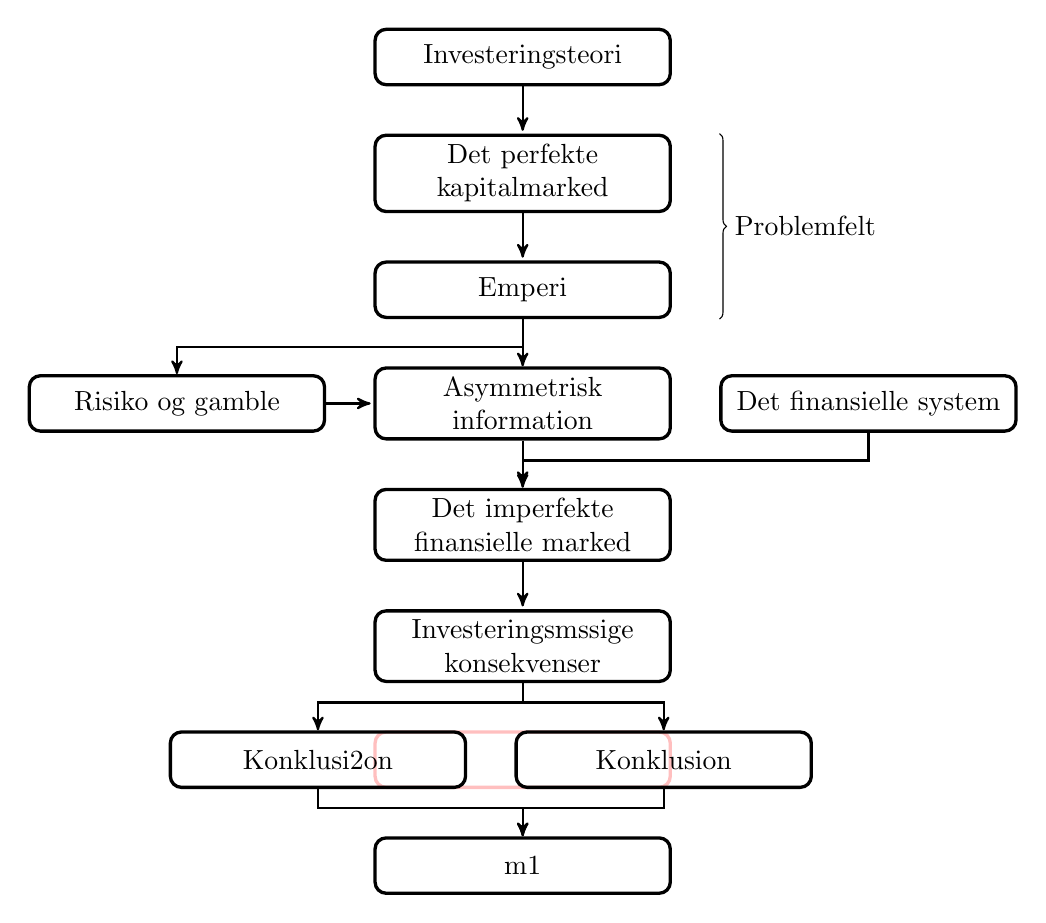
\begin{tikzpicture}
	[node distance=.6cm,
	start chain=going below,]

	\node[punktchain, join] (investeringer)      {Investeringsteori};
	\node[punktchain, join] (perfekt) {Det perfekte kapitalmarked};
	\node[punktchain, join, ] (emperi) {Emperi};
	\node (asym) [punktchain ]  {Asymmetrisk information};
	\begin{scope}[start branch=venstre,
	%We need to redefine the join-style to have the -> turn out right
	every join/.style={->, thick, shorten <=1pt}, ]
	\node[punktchain, on chain=going left, join=by {<-}]
	(risiko) {Risiko og gamble};
	\end{scope}
	\begin{scope}[start branch=hoejre,]
	\node (finans) [punktchain, on chain=going right] {Det finansielle system};
	\end{scope}
	\node[punktchain, join,] (disk) {Det imperfekte finansielle marked};
	\node[punktchain, join,] (makro) {Investeringsmssige konsekvenser};
		\node[punktchain, draw=pink] (aux1) { };
	\node[punktchain, below right=0.6cm and -2cm of makro] (konk) {Konklusion};
	\node[punktchain,  left = of konk,] (konk2) {Konklusi2on};
		\node[punktchain, below= of aux1 ] (m1) {m1};
	% Now that we have finished the main figure let us add some "after-drawings"
	%% First, let us connect (finans) with (disk). We want it to have
	%% square corners.
	\draw[|-,-|,->, thick,] (finans.south) |-+(0,-1em)-| (disk.north);
	\draw[|-,-|,->, thick,] (emperi.south) |-+(0,-1em)-| (risiko.north);
	\draw[|-,-|,->, thick,] (emperi.south) |-+(0,-1em)-| (asym.north);

\draw[|-,-|,->, thick,] (makro.south) |-+(0,-0.7em)-| (konk.north);
\draw[|-,-|,->, thick,] (makro.south) |-+(0,-0.7em)-| (konk2.north);

\draw[|-,-|,->, thick,] (konk.south) |-+(0,-0.7em)-| (m1.north);
\draw[|-,-|,->, thick,] (konk2.south) |-+(0,-0.7em)-| (m1.north);

	% Now, let us add some braches. 

	\draw[tuborg, decoration={brace}] let \p1=(perfekt.north), \p2=(emperi.south) in
	($(2.5, \y1)$) -- ($(2.5, \y2)$) node[tubnode] {Problemfelt};
	\end{tikzpicture}
		\begin{itemize}
			\item Designing research Creswell
			
		\end{itemize}
	%%%%%%%%%%
	\section{Literature Review}
	%%%%%%%%%%
		\begin{itemize}
			\item Where, How, For what
		\end{itemize}
	%%%%%%%%%%
	\section{Empirical Research}
	%%%%%%%%%%
		\begin{itemize}
			\item Qualitative Methods
			\item Interviews, how many, how long, with whom, sample
		\end{itemize}
	%%%%%%%%%%
	\section{Design Science}
		\begin{itemize}
			\item Hefner, Peffers. Draw line complete the view of used research methods.
		\end{itemize}
%%%%%%%%%%
\chapter{Research Background}
	%%%%%%%%%%
	DEFINITIONS DEFINITIONS DEFINITIONS
	\section{Domain}
	%%%%%%%%%%
	

	
		%%%%%%%%%%
		\subsection{Business Process Outsourcing}
		%%%%%%%%%%
		\begin{itemize}
			\item BPO with PO
			\item offshore, nearshore, inshore
		\end{itemize}
		%%%%%%%%%%
		\subsection{Customer Management}
		%%%%%%%%%%
		\begin{itemize}
			\item CSM or CM?
			\item Value Chain
			\item Importance for businesses
		\end{itemize}
		%%%%%%%%%%
		\subsection{Customer Management Business Process Outsourcing Providers}
		%%%%%%%%%%
		\begin{itemize}
			\item Strategy, Capabilities
			\item B2B2X
			\item virtual company
		\end{itemize}
	%%%%%%%%%%
	\section{Reference Modeling}
	%%%%%%%%%%
		%%%%%%%%%%
		\subsection{Concept}
		%%%%%%%%%%
		%%%%%%%%%%
		\subsection{Benefits}
		%%%%%%%%%%
		%%%%%%%%%%
		\subsection{icebricks as a means}
		%%%%%%%%%%
\chapter{Case}
%%%%%%%%%%
%%%%%%%%%%
\section{DSR Application for Arvato}
%%%%%%%%%%
%%%%%%%%%%
\section{Problem Identification}
%%%%%%%%%%
%%%%%%%%%%
\section{Solution Objective and Stakeholders}
%%%%%%%%%%
%%%%%%%%%%
\section{Limitiations}
%%%%%%%%%%
%%%%%%%%%%

\chapter{Reference Model Construction}
%%%%%%%%%%
%%%%%%%%%%
\section{Process Framework}
%%%%%%%%%%
%%%%%%%%%%
\section{Internal Services}
%%%%%%%%%%
%%%%%%%%%%
\subsection{...}
\section{Client Services}
\subsection{...}
\section{Customer Services}
\subsection{...}
\chapter{Evaluation}
\section{Internal Services}
\section{Client Services}
\section{Customer Services}
\chapter{Conclusion}






\chapter{Sample}
This \LaTeX \- template has been developed as an alternative to the well-known Microsoft Word \enquote{Becker-Vorlage}. \path{00_thesis.tex} is the master file.

It is build by  Jan Betzing and Dominik Lekse and draws from the DBIS template by Till Haselmann and Florian Stahl, as well as from the IS template by Stephan Dlugosz.

This document is work-in-progress and provides instructions on how to use the template. It does not give advices on scientific writing.

Please feel free to contribute to this template. Members of the WWU M\"{u}nster can request access to the template by contacting the author at \href{mailto:jan.betzing@ercis.uni-muenster.de}{jan.betzing@ercis.uni-muenster.de}. Afterwards you will be able to clone the template from \path{https://wiwi-gitlab.uni-muenster.de/lsis/isthesis.git}, and create push-requests with their new features.

\paragraph{TODO}
\begin{itemize}
	\item Configuration switch for having \textbackslash chapter\{\} begin on a new page
	\item Replace \texttt{kvoptions} with \texttt{pgfkeys}
\end{itemize}
\section{Elements}
This chapter gives examples on what you can do with this template. It's just a brief overview. Please consult the common sources on how to write sicentific documents and documents with \LaTeX.

\section{Structure}
This template provides three structural levels that appear in the table of contents, \viz, \texttt{\textbackslash chapter}, \texttt{\textbackslash section}, and \texttt{\textbackslash subsection}. Chapters will always start on a new page. Additionally, you can use \texttt{\textbackslash subsubsection} and \texttt{\textbackslash paragraph} as non-hierarchical means to structure your thesis.


\subsection{Lists}
You can use the default \LaTeX \- functions for writing lists, \viz, \texttt{\textbackslash enumerate} for numbered lists and \texttt{\textbackslash itemize} for bullet point lists. Again, the \texttt{\textbackslash subsubsection} and \texttt{\textbackslash paragraph} can be used as structural elements, \eg, when listing definitions of terms.

\subsection{Footnotes}
Footnotes are contiguously numbered throughout the whole document. Use the \texttt{\textbackslash footnote\{text\}} command.  They appear on the page their reference is on \footnote{This is an exemplary footnote.}. Footnotes have to be placed without whitespace behind the word and within the sentence boundaries, \ie, before the period.

\subsection{ToDo-Notes}
You can use ToDo notes using the \texttt{\textbackslash todo\{text\}}  command. Please make sure to remove any ToDo notes before handing in your thesis! \todo[inline]{ToDo: Remove me before publishing}

\section{Formatting Text}
\LaTeX \- provides \texttt{\textbackslash textit\{text\}} for \textit{italics}, \texttt{\textbackslash textbf\{text\}} for \textbf{bold face}, \texttt{\textbackslash texttt\{text\}} for \texttt{typewriter}, \texttt{\textbackslash textsc\{text\}} for \textsc{small caps}, \texttt{\textbackslash underline\{text\}} for \underline{underline}. Additionally, the template provides  \texttt{\textbackslash texthl\{text\}} for \texthl{highlighted text}. Please remove any highlighted text before handing in your thesis!

Please use the \texttt{\textbackslash enquote\{text\}} command for \enquote{direct quotes}.

\subsection{Colors}
This template comes with the colors defined in the \glspl{CD} of the \acrshort{ERCIS} and \acrshort{WWU}. \Tab \ref{tab:colors} lists the color names. You can apply them to text by using the  \\ \texttt{\textbackslash textcolor\{color name\}\{text\}} command.
	
\begin{table}[caption={Colors defined by the template}, label=tab:colors]
	\centering
		\begin{tabular}{@{}ll@{}}
			\toprule
			{\bf Color Name} & {\bf Result} \\ \midrule
			ercis-black      & \textcolor{ercis-black}{Exemplary Text and 0123456789}  \\
			ercis-grey      & \textcolor{ercis-grey}{Exemplary Text and 0123456789}  \\
			ercis-red      & \textcolor{ercis-red}{Exemplary Text and 0123456789}  \\
			ercis-lightred      & \textcolor{ercis-lightred}{Exemplary Text and 0123456789}  \\
			ercis-blue      & \textcolor{ercis-blue}{Exemplary Text and 0123456789}  \\
			ercis-darkblue      & \textcolor{ercis-darkblue}{Exemplary Text and 0123456789}  \\
			ercis-cyan    & \textcolor{ercis-cyan}{Exemplary Text and 0123456789}  \\
			ercis-orange      & \textcolor{ercis-orange}{Exemplary Text and 0123456789}  \\
			ercis-green      & \textcolor{ercis-green}{Exemplary Text and 0123456789}  \\ \midrule
			wwu-black      & \textcolor{wwu-black}{Exemplary Text and 0123456789}  \\
			wwu-green      & \textcolor{wwu-green}{Exemplary Text and 0123456789}  \\
			wwu-lightgreen      & \textcolor{wwu-lightgreen}{Exemplary Text and 0123456789}  \\
			wwu-blue     & \textcolor{wwu-blue}{Exemplary Text and 0123456789}  \\
			wwu-lightblue      & \textcolor{wwu-lightblue}{Exemplary Text and 0123456789}  \\ \bottomrule
		\end{tabular}
\end{table}


\section{Figures}

The \texttt{figure} environment is wrapped around images. These images should either be included as PDF-file via \texttt{\textbackslash includegraphics}, or created via \textit{TikZ/PGF}. For included images, make sure to use high-resolution images, preferably vector images.

Figures float, \ie, they do not necessarily appear at exact the same position you have defined them. Make sure to set a  \textit{caption} and an optional \textit{label} as figure parameters. 

\begin{figure}[caption={Relationship of students and theses}, label={fig:img01}]
	{	
\includegraphics[width=.6\textwidth]{figures/figure01.pdf}}
\end{figure}

\subsection{Subfigures}
Sometimes it might be handy to contrast figures, \ie, by placing them next to each other. The template uses the \textit{subcaption} package to provide subfigures. The following example contains two figures, where each subfigure has its own \texttt{\textbackslash label} and \texttt{\textbackslash caption}. Additionally, the whole figure has its own \textit{caption} and \textit{label}. That means, you can reference subfigures  \fig \ref{fig:subfig1} and \fig  \ref{fig:subfig}. Only the whole figure will be listed in the table of figures.

Subfigures are not limited to images, but may also include listings or tables. \Fig \ref{fig:subfig} shows a sample database query expressed in \ac{SQL} (\fig \ref{fig:subfig1}) and as query plan in relational algebra  (\fig \ref{fig:subfig2}).
 
\begin{figure}[caption={Exemplary use of subfigures}, label={fig:subfig}]
	
	\begin{subfigure}[b]{.45\textwidth}
		
		\begin{lstlisting}[nolol, language=SQL]
		SELECT b, d FROM 
			EXAMPLE.RELATION1 r,
			EXAMPLE.RELATION2 s,
		WHERE 
			r.a = 'c'
		AND 
			s.e = 2
		AND 
			r.c = s.c; 
		\end{lstlisting}
		\caption{\gls{SQL} select statement}\label{fig:subfig1}
	\end{subfigure}
	\begin{subfigure}[b]{.53\textwidth}
		\centering	
		\begin{tikzpicture}[node distance = 2cm, auto,
		database/.style={
			cylinder,
			cylinder uses custom fill,
			cylinder body fill=gray!30,
			cylinder end fill=gray!20,
			shape border rotate=90,
			aspect=0.25,
			draw
		}]
		\node [] (queue) {$\Pi_{b, d}$};
		\node [below of=queue] (join) {$\Join_{r.c = s.c}$};
		
		\node [below left of=join,xshift=-1cm] (l1) {$\sigma_{r.a = 'c'}$};
		\node [database, below of=l1] (l2) {\texttt{r}};
		
		\node [below right of=join,xshift=1cm] (r1) {$\sigma_{s.e = 2}$};
		\node [database,below of=r1] (r2) {\texttt{s}};
		
		\draw [<-] (queue) -- (join);
		\draw [<-] (join) -- (r1);
		\draw [<-] (r1) -- (r2);
		\draw [<-] (join) -- (l1);
		\draw [<-] (l1) -- (l2);
		\end{tikzpicture}
		\caption{Sample evaluation plan}\label{fig:subfig2}
	\end{subfigure}
\end{figure}
\section{Listings}
You can use listings to typeset source code. This template uses the \textit{listings} package. Wrap code inside the \texttt{lstlisting} environment and set the \textit{language} (e.g., Java, SQL), \textit{caption}, and optional \textit{label} parameters. If the source code highlighting highlights the wrong keywords or misses keywords, use the \textit{deletekeywords} \resp \textit{morekeywords} parameters. Consult the package documentation for further information.

\begin{lstlisting}[float=htp, caption={Euclid's GCD algorithm implemented in Java}, label={lst:euclid}, language=Java, deletekeywords={}, morekeywords={}]
public class Euclid {

	public static int gcd(int p, int q) {
		if (q == 0) return p;
		else return gcd(q, p % q);
	}

}
\end{lstlisting}

\section{Algorithms}
Some users might require specifying algorithms. This template uses the \textit{algorithm}, \textit{algorithmicx}, and \textit{algopseudocode} packages. Consult the respective manuals for further information. Algorithms do not appear in a table at the beginning of the document, \ie, there is no list of algorithms.

\begin{algorithm}[htb]
	\begin{algorithmic}
		\Require nonnegative integer $a$, nonnegative integer $b$
		\Function{Euclid}{$a, b$}
		\If {$b = 0$} \Comment{comment}
		\State{return $a$;}
		\Else 
		\State {return \textsc{Euclid}$(b, a\mod b)$;}
		\EndIf
		\EndFunction
	\end{algorithmic}
	\caption{Euclid's GCD algorithm in pseudocode}
	\label{alg:garbage}
\end{algorithm}

\section{Acronyms and Abbreviations}
This template provides comprehensive support for acronyms and abbreviations. The template uses the \textit{glossaries} package. 
Please do only define abbreviations and symbols that are uncommon. That means, common abbreviations such as \enquote{\eg} or \enquote{\ie} should not be listed. Abbreviations and symbols are sorted automatically by their label. 

\subsection{Common Abbreviations}
Please note that each full stop in a common abbreviation should be followed by a non-breaking space. This template comes with a variety of macros for common abbreviations, that can be used throughout your theses. The macros differ for English and German theses. Please see the tables below.

\begin{table}[caption={Common abbreviation macros for English theses}, label=tab:macros1]
	\centering
	\begin{tabular}{@{}ll@{}}
		\toprule
		{\bf Command} & {\bf Result} \\ \midrule
			\textbackslash apprx      & \apprx \\
			\textbackslash as      & \as \\
			\textbackslash cf      & \cf \\
			\textbackslash eg      & \eg \\
			\textbackslash Eg      & \Eg \\
			\textbackslash esp      & \esp \\
			\textbackslash etal      & \etal \\
			\textbackslash fig      & \fig \\
			\textbackslash Fig     & \Fig \\
			\textbackslash ie      & \ie \\
			\textbackslash Ie      & \Ie \\
			\textbackslash iid      & \iid \\
			\textbackslash p\{4711\}      & \p{4711} \\
			\textbackslash pf\{4711\}      & \pf{4711} \\
			\textbackslash pp\{11$--$47\}      & \pp{11--47} \\
			\textbackslash resp      & \resp \\
			\textbackslash sect     & \sect \\
			\textbackslash tab      & \tab \\
			\textbackslash Tab      & \Tab \\
			\textbackslash viz      & \viz \\
			\textbackslash wrt      & \wrt \\ \bottomrule
	\end{tabular}
\end{table}

\begin{table}[caption={Common abbreviation macros for German theses}, label=tab:macros2]
	\begin{subfigure}[t]{.45\textwidth}
	\centering
	\begin{tabular}{@{}ll@{}}
		\toprule
		{\bf Command} & {\bf Result} \\ \midrule
\textbackslash aaO & \mbox{a.\,a\,O}\xdot \\
\textbackslash Abb & \mbox{Abb.~} \\
\textbackslash bspw & \mbox{bspw}\xdot \\
\textbackslash bzgl & \mbox{bzgl}\xdot \\
\textbackslash bzw & \mbox{bzw}\xdot \\
\textbackslash ca & \mbox{ca}\xdot \\
\textbackslash dgl & \mbox{dgl}\xdot \\
\textbackslash dsgl & \mbox{dsgl}\xdot \\
\textbackslash dh & \mbox{d.\,h}\xdot \\
\textbackslash etc & \mbox{etc}\xdot \\
\textbackslash eV & \mbox{e.\,V}\xdot \\
\textbackslash evtl & \mbox{evtl}\xdot \\
\textbackslash fs & \mbox{f.\,s}\xdot \\
\textbackslash gdw & \mbox{g.\,d.\,w}\xdot \\
\textbackslash ggf & \mbox{ggf}\xdot \\
\textbackslash hc & \mbox{h.\,c}\xdot \\
\textbackslash iAllg & \mbox{i.\,Allg}\xdot \\
\textbackslash iBa & \mbox{i.\,B.\,a}\xdot \\
\textbackslash idR & \mbox{i.\,d.\,R}\xdot \\
\textbackslash ieS & \mbox{i.\,e.\,S}\xdot \\
\textbackslash inkl & \mbox{inkl}\xdot \\
\textbackslash insb & \mbox{insbes}\xdot \\
\textbackslash Prof & \mbox{Prof}\xdot \\
\textbackslash Dr & \mbox{Dr}\xdot \\
\textbackslash PD & \mbox{PD}\xdot \\
\textbackslash Ing & \mbox{Ing}\xdot \\
\textbackslash iV & \mbox{i.\,V}\xdot \\
\textbackslash iW & \mbox{i.\,W}\xdot \\
\textbackslash iwS & \mbox{i.\,w.\,S}\xdot \\
\textbackslash Nr\{123\} & \mbox{Nr.~123} \\
\textbackslash nW & \mbox{n.\,W}\xdot \\
\textbackslash oa & \mbox{o.\,a}\xdot \\
\textbackslash oAe & \mbox{o.\,\"{A}}\xdot \\
			\textbackslash oae & \mbox{o.\,\"{a}}\xdot \\\bottomrule
\end{tabular}
\end{subfigure}
	\begin{subfigure}[position=t]{.45\textwidth}
		\centering
		\begin{tabular}{@{}ll@{}}
			\toprule
			{\bf Command} & {\bf Result} \\ \midrule

			\textbackslash oE & \mbox{o.\,E}\xdot \\
			\textbackslash oEdA & \mbox{o.\,E.\,d.\,A}\xdot \\
			\textbackslash OEdA & \mbox{O.\,E.\,d.\,A}\xdot \\ 
			\textbackslash oV & \mbox{o.\,V}\xdot \\
			\textbackslash OV & \mbox{O.\,V}\xdot \\
			\textbackslash resp & \mbox{resp}\xdot \\
			\textbackslash S\{123\} & \mbox{S.~123} \\
			\textbackslash Sf\{123\} & \mbox{S.~123~f}\xdot \\
			\textbackslash Sff\{123\} & \mbox{S.~123~ff}\xdot \\
			\textbackslash siehe & \mbox{s.\,o}\xdot \\
			\textbackslash sog & \mbox{sog}\xdot \\
			\textbackslash sS\{123\}  & \mbox{s.\,S.~123}\\
			\textbackslash sSf\{123\} &\mbox{s.\,S.~123~f}\xdot \\
			\textbackslash sSff\{123\}& \mbox{s.\,S.~123~ff}\xdot \\
			\textbackslash stu & \mbox{st.\,u}\xdot \\
			\textbackslash su & \mbox{s.\,u}\xdot \\
			\textbackslash Tab & \mbox{Tab.~} \\
			\textbackslash tw & \mbox{t.\,w}\xdot \\
			\textbackslash ua & \mbox{u.\,a}\xdot \\
			\textbackslash etal & \mbox{et\ al}\xdot \\
			\textbackslash uae & \mbox{u.\,\"{a}}\xdot \\
			\textbackslash uAe & \mbox{u.\,\"{A}}\xdot \\
			\textbackslash uiv & \mbox{u.\,i.\,v}\xdot \\
			\textbackslash usw & \mbox{usw}\xdot \\
			\textbackslash uU & \mbox{u.\,U}\xdot \\
			\textbackslash va & \mbox{v.\,a}\xdot \\
			\textbackslash vgl & \mbox{vgl.~} \\
			\textbackslash Vgl & \mbox{Vgl.~} \\
			\textbackslash vs & \mbox{v.\,s}\xdot \\
			\textbackslash zB & \mbox{z.\,B}\xdot \\
			\textbackslash zT & \mbox{z.\,T}\xdot \\
			\textbackslash zz & \mbox{zz}\xdot \\
			\textbackslash zzgl & \mbox{zzgl}\xdot \\
 & \\ \bottomrule
	\end{tabular}
	\end{subfigure}
\end{table}

\subsection{Custom Abbreviations}
Custom abbreviations are defined in the \path{acronyms.tex} file, using the \\
\texttt{\textbackslash newacronym[longplural=\{<long plural>\}, shortplural=\{<short plural>\}]\\ \{<label>\}\{<short>\}\{<long>\}} command. The \textit{longplural} and \textit{shortplural} parameters are optional. The abbreviations are sorted by their labels. The label is furthermore used to reference the abbreviations in your text. You can do so using commands listed in \tab \ref{tab:glossaries}. In most cases, you just use \textbackslash gls\{<label>\}. On the first occurrence, the full version is displayed, \eg, \acrfull{ERCIS}. Afterwards, the short version will be displayed, \eg, \acrshort{ERCIS}.

You pluralize your abbreviation by adding a \texttt{pl} to the \resp command. This will add a small s to the abbreviation, \eg, \acrshortpl{CD}. \Tab \ref{tab:glossaries} shows custom short and long plural versions of the abbreviation \acrshort{kmu}. You might need this \esp for more complex German abbreviations that do not have a \enquote{s} plural form.

\begin{table}[caption={Commands for printing abbreviations}, label=tab:glossaries]
	\centering
	\begin{tabular}{@{}ll@{}}
		\toprule
		{\bf Command} & {\bf Result} \\ \midrule
		\textbackslash gls\{<label>\}     & \textbackslash acrfull on first occurence, \textbackslash acrshort otherwise \\
		\textbackslash glspl\{<label>\}       &  \textbackslash acrfullpl on first occurence, \textbackslash acrshortpl otherwise \\
		\textbackslash acrshort\{<label>\}       & \acrshort{kmu} \\
		\textbackslash acrshortpl\{<label>\}       & \acrshortpl{kmu} \\
		\textbackslash acrlong\{<label>\}       & \acrlong{kmu} \\
		\textbackslash acrlongpl\{<label>\}      & \acrlongpl{kmu} \\
		\textbackslash acrfull\{<label>\}      & \acrfull{kmu} \\
		\textbackslash  acrfullpl\{<label>\}     & \acrfullpl{kmu} \\ \bottomrule
	\end{tabular}
\end{table}

Only referenced abbreviations will be added to the list of abbreviations.

\subsection{Symbols}
If required, you can define symbols in the \path{symbols.tex} file, using the \\ \texttt{\textbackslash addsymboltolist\{<symbol>\}\{<label>\}\{<name>\}} command. The symbols are sorted by their labels. Please note, regardless of using the symbols in the text, all symbols defined in the symbols file will be output to the list of symbols.

\section{Citations and Bibliography}
This template uses {BibTeX} for bibliographies. It comes with the MISQ style that takes care of proper formating and sorting of your references. Of course, you have to maintain a clean \path{.bib} file that caters all necessary attributes. References will appear in the alphabetical order of the surname of the first author. In case of several works by the same author, they are sorted by year.

Citing in the text is done with the \textbackslash citep[<before>][<after>]\{<citekey>\} command. Citations without parenthesis are done with \textbackslash cite\{<citekey>\}. You can reference authors with \textbackslash citeauthor\{<citekey>\}. However, we suggest typesetting authors in \textsc{Small Caps}, \eg, \textsc{\citeauthor{Hammer2015}} is one father of \ac{BPM}.

\paragraph{Exemplary citations}

\begin{itemize}
	\item \gls{BPM} is an integral management paradigm for building and running effective and efficient organizations  \citep{Hammer2015, VomBrocke2014a}.
	\item A holistic approach to \ac{BPM} goes beyond process modeling and workflow management systems \citep[\p{530}]{VomBrocke2014a}.
	\item See \cite{VomBrocke2014a} for a comprehensive review on \ac{BPM} best practices.
	\item \textsc{\citeauthor{Hammer2015}} lists organizational capabilities for \ac{BPM} \citep[\cf][\pf{9}]{Hammer2015}, while \textsc{vom Brocke} \etal give principles of good \ac{BPM} \citep[\cf][\pp{530--546}]{VomBrocke2014a}.
	\item Two authors are automatically divided by an \enquote{and} in English or an \enquote{und} in German, \eg, \citep{Becker2011}.
	\item \enquote{\ac{BPM} can provide a solid set of capabilities essential to master contemporary and future challenges} \citep[\p{534}]{VomBrocke2014a}.
\end{itemize}

\subsection{Misc}
The name and matriculation number of the student will automatically be displayed on the header of every page when the thesis type \textit{seminar} is selected.

\chapter{Compiling the document}
In order to generate a PDF-file from your \TeX-file you have to run the following commands. We assume you have a master file \path{00_thesis.tex} that you want to typeset.

\begin{lstlisting}[float=htp, caption={Commands to compile this document}, label={lst:compiling}, language=bash, morekeywords={pdflatex, bibtex, makeglossaries}]
pdflatex 00_thesis
pdflatex 00_thesis
makeglossaries 00_thesis
bibtex 00_thesis
pdflatex 00_thesis
pdflatex 00_thesis
\end{lstlisting}

Alternatively, you can use your favorite task runner. This thesis comes with a \textit{Grunt} file to kick-start your \LaTeX writing.

When running, Grunt will monitor your thesis and on file changes, the PDF-file is automatically rebuild using the commands from listing \ref{lst:compiling}.
 
Please make sure to have node.js and the \gls{npm} installed. Now you can open a command prompt at the document root and run the commands in listing \ref{lst:grunt}. 

\begin{lstlisting}[float=htp, caption={Installing and running Grunt}, label={lst:grunt}, language=bash]
# Install Grunt via npm (use sudo on Unix-based OS)
npm install -g grunt-cli

# Install Grunt plugins / dependencies
npm install

# Run the Grunt listener 
grunt
\end{lstlisting}

\section{Known Issues}
Under some configurations on Windows machines, the \texttt{makeglossaries} command silently fails, which results in empty lists of accronyms and symbols. Same goes for the implicitly called \texttt{makeindex} command. In this case, you have to install \texttt{Perl}\footnote{https://www.perl.org/get.html} on your machine.
		%!TEX root = ./00_thesis.tex
%!GEDIT texmaster = ./00_thesis.tex
% !TeX spellcheck = en_US
\chapter{Motivation}

Prozessorientierung ist eine nicht mehr wegzudenkende Maxime in der Gestaltung von Unternehmen. Sie ist ein wesentlicher Bestandteil der Forschung in der Be- triebswirtschaftslehre und der Wirtschaftsinformatik.
As put by Thomas Friedman, "The world is flat". Globalization facilitates combinations value-creating activities in economic networks like never before. The key driver of it is information technology, which sets the base for the connectedness we take for granted today. Its implications on markets and businesses are described in the following section. 

Reference modeling is a central disciple in IS research \cite{Fettke2004, konig1996entwicklung, becker2004handelsinformationssysteme}. It refers to the use and construction of reference models.

vorhoef, lemon!!



Process orientiation is a precept in business organization. It is an essential part of research in business adminstration as well as \acrfull{IS}. To make use of it, models as the language of \acrshort{IS} take an important part. In particular, the reference models support businesses in these reorganization projects. They guide the user and help to incorporate best and common practices so that there is solid foundation to customize the model for the businesse's originalities.  

Outsourcing customer service to external providers is a common practice throughout many industries. Dialling a contact number for a service request often ends up with talking to a service agent anywhere around the world. Several companies have specialized to provide professional customer support using various contact channels. Providing customer relationship management (CRM) as service requires the careful and cost-efficient deployment of contact centres. Such centres are often staffed with hundreds of agents that must be hired and trained before customer contact.
For years, special focus has been put on the voice channel (Loudhouse, 2013). Meanwhile digital trends have affected many areas of life, which implies new challenges in customer relationship management. A recent study revealed that 78.7\% of call centre operations managers point out that their current systems fail to meet future needs, as they are telephone-centric and costs for an architecture overhaul are too high (Dimension Data, 2015). Nowadays consumers can use a plethora of devices and software applications to interact with organizations (Köffer, Ortbach and Niehaves, 2014). As a result, the number of used channels to reach organizations increases. More specifically, analysts have seen a move from the traditional voice channel to digital channels, such as chat or social media. For instance, private instant messengers offer faster and less complicated ways to interact with the company. Digital channels in contact centres now take 42\% of overall interactions and are said to overtake voice by the end of 2016 (Dimension Data, 2016). To this end, multichannel CRM has become a “must-have” for customer service management providers (Agnischock et al., 2015).
In this context, the term omnichannel CRM is increasingly dragging intention. Omnichannel CRM can be distinguished from multichannel CRM by not only providing multiple channels for customer interaction but also through seamless integrations of various channels and their underlying data (Verhoef, Kannan and Inman, 2015), which is a difficult task in CRM. At this point in time, omnichannel CRM is often not realized. However, customers more and more expect that they are able to switch between interaction channels without the loss of information. Contact centre interactions will often require the customer to repeat information again, although he or she has earlier written an email or a chat message to the same company.
Omnichannel CRM also comes with important benefits for organizations. Integrated data throughout various channels allows getting a better understanding of the customer’s profile and wishes through analytical support. Still, 40\% of contact centres have no data analysis tool in place despite of being named the top factor to shape the industry in the next five years (Dimension Data, 2015). 
To this end, organizations can better target marketing campaigns or increase the quality of service provision. To realize this, organizations that use outsourcing need close relations to outsourcing providers, since the integration of channels affects various information systems both at the organization but also at the outsourcing provider. More specifically, CRM business processes need to be harmonized since they often span organizational boundaries.


 

Outsourcing processes have be



	\begin{itemize}
		\item Janina BA
		\item ECIS Paper
		\item Refmod motivation Püster?
		\item Omnichannel 
		\item purpose statement
		\item research question and hyptoheses
	\end{itemize}

	\begin{itemize}
		\item Crewsell: State problem, 
		\item review studies that have addressed the problem,
		\item  indicate definciencies in studies, 
		\item advance significance, 
		\item state purpose statement
	\end{itemize}
%%%%%%%%%%

		\chapter{Methodology}
%%%%%%%%%%
This chapter outlines the underlying methodology of this work. Following \cite{gilljohnson}, the sequence of a research process is identify area (1), select research topic (2), decide on approach (3), formulate plan (4), collect data (5),  analyze data (6), present findings (7). With the first two steps being motivated and further specified in \ref{chap:case}, this section especially reasons approach (3), plan (4) and data aspects (5). 

This thesis is part of a wider research project targeting processes, data and analytics in omni-channel CRM. The methodology described in the following refers to this thesis only and not to the superordinate research project. Prior work in the project helped to create a foundation where this work can build on. \acrfull{DSR} is chosen as the research design, which is described in detail in the following sections, along with the epistemological aspects. Data was gathered in interviews with domain experts, supported by literature, as well as documents from the research partner. Descriptions of these data sources complete this chapter. 


	\section{Epistemological Perspective}
	%%%%%%%%%%		
Stating the epistemological view of this work helps to support the reader in understanding the author's statements. Furthermore, it demonstrates a systematical method, which is sometimes perceived as lacking in qualitative research. Drawing on a framework by \cite{becker2007epistemological}, five questions are mentioned in order to structure the epistemological positioning of research. The concepts highlighted in bold represent the approach taken in this thesis. 

\begin{enumerate}
	\item What is the object of cognition? (Ontological aspect)
		\subitem \textbf{Ontological Realism} | Ontological idealism  | Kantianism
	\item What is the relationship between cognition and the object of cognition?
		\subitem Epistemological realism | \textbf{Constructivism}
	\item What is true cognition? (Concept of truth)
		\subitem Correspondence |  \textbf{Consensus} |  Semantic theory of truth
	\item Where does cognition originate?
	\subitem Empiricism | Rationalism | \textbf{Kantianism}
	\item By what means can cognition be achieved? (Methodological aspect)
		\subitem \textbf{Inductivism} | \textbf{Deductivism} | \textbf{Hermeneutic}
\end{enumerate}

%\begin{table}[caption={Epistemological perspective}, label=fig:epi]
%	\centering
%	\begin{tabular}{|p{6cm}|p{1.5cm}|p{1.5cm}|p{1.5cm}|p{1.5cm}|p{1.5cm}|p{1.5cm}|}
%		\hline
%		\textit{What is the object of cognition? (Ontological aspect)}                   & \multicolumn{2}{l|}{\textbf{Ontological Realism}} & \multicolumn{2}{l|}{Ontological idealism} & \multicolumn{2}{l|}{Kantianism}               \\ \hline
%		\textit{What is the relationship between cognition and the object of cognition?} & \multicolumn{3}{l|}{Epistemological realism}                            & \multicolumn{3}{l|}{\textbf{Constructivism}}                        \\ \hline
%		\textit{What is true cognition? (Concept of truth)}                              & \multicolumn{2}{l|}{Correspondence}               & \multicolumn{2}{l|}{\textbf{Consensus}}   & \multicolumn{2}{l|}{Semantic theory of truth} \\ \hline
%		\textit{Where does cognition originate?}                                         & \multicolumn{2}{l|}{Empiricism}                   & \multicolumn{2}{l|}{Rationalism}          & \multicolumn{2}{l|}{\textbf{Kantianism}}      \\ \hline
%		\textit{By what means can cognition be achieved? (Methodological aspect)}        & \multicolumn{2}{l|}{\textbf{Inductivism}}         & \multicolumn{2}{l|}{\textbf{Deductivism}} & \multicolumn{2}{l|}{\textbf{Hermeneutic}}     \\ \hline
%	\end{tabular}
%
%\end{table}

\subsubsection{Ad 1. Object of cognition}
Ontology is the science of \textit{what is} and \textit{how it is}. The existence and nature of reality are subject matter. Ontological realism assumes a real world that exists independently of cognition. Ontological idealism sees reality as a construct depending on human consciousness. Kantianism brings together the two mentioned views by distinguishing in the unknowable \enquote{thing-in-itself} and the appearing of those things to an observer. 

This work takes the view of ontological realism, as the construction of the reference model is intended to solve a real-world problem. Hence, this world should exist for every observer. 

\subsubsection{Ad 2. Relationship between cognition and the object of cognition}
This question asks whether entities beyond human thought can be recognized as objective (in principle). Epistemological realism affirms this question. Constructivism deems cognition as subjective and hence makes understanding a private construct determined by the subject. 

Because subjects that turn the reference model to account will show different understandings and requirements, the constructivistic view is taken. These subjects can be classified into reference model users and designers, that will see it from different angles from a group perspective, \eg scientific and practical. Moreover, every subject will interpret the model in a subjective manner.

\subsubsection{Ad 3. Concept of truth}
The \textit{true} cognition and how humans can achieve it is foci of this question and there are three theories \citep{habermas1973}. Correspondence theory of truth states that true statements refer to facts of the real world. This requires a realistic view in both ontology and epistemology. Consensus theory of truth bases on constructivism: A statement is true\textit{ for a group}, only if all peers agree and true if everyone agrees. Hence there can be no proof of truth. Thirdly, semantic theory of truth proposes that truth is always related to an object language where the possibly true statements are communicated in. Therefore there has to be a meta-language that is able to analyze the correctness of a statement in object language \citep{tarski1944}. 

Following the constructivistic view, the consensus theory of truth is selected. The correctness of modeling is dependent on the group of reference model users and its designers. If they find a consensus, truth can be achieved within the group. Application of the reference model changes the user group and implies changes in the model, so that it matches the circumstances in the company. The application model designers and users then again need to find a consensus.

\subsubsection{Ad 4. Origin of cognition}
There are three origins of cognition. Cognition from experience falls under the school of empiricism. Rationalism puts intellect as the source of cognition. Kantianism again combines both views so that both experience and intellect can be origin of cognition. 

Both intellect and experience are seen as integral parts of cognition in research. Cognitive efforts and reflections of the author are part of the reference model design. Practical experience, as included by the interview component, is used for evaluating the artifact. This requires avoiding direct use of interview content in artifact design, so that a self-fulfilling prophecy is prevented. 

\subsubsection{Ad 5. Methodological aspect}
While inductivism describes the extension from individual cases to universal laws, deductivism is the derivation of the individual from the universal \citep{seiffert2006einfhrung}. Hermeneutic assumes prior knowledge in an issue by a subject that is able to improve its understanding of \textit{the entire} by consumption of new knowledge. This repeating consumption shapes understanding and is called the hermeneutic cycle \citep{Butler1998}.

Inductivism is focal in reference modeling, as the case needs to be abstracted to achieve the required universality in reference modeling. Deductivism is also part, as general process  structures were applied to the domain of BPO and more specifically BPO in CRM. Both are common in construction of reference models \citep{thomas2006mang,Fettke2014meth}.

The act of design within this work is characterized by a hermeneutic aspect. The model is shaped by the consumption of existing scientific concepts, as well as requirements from the practical case. As the approach was to increase modeling detail over time, a repeating process emerged: First interviews derived high-level requirements, while the following gave new input that related to additional knowledge. This additional knowledge closes the circle as it became preknowledge to the next repetition. 

%%%%%%%%%%
\section{Design Science}
Research has to employ accepted methodologies to be accepted in the community. \citeauthor{creswell2013research} names the selection of a research approach as the first of preliminary considerations \citep{creswell2013research}. \acrfull{DSR}, as conceptualized by \cite{simon1996sciences} is getting more and more attention in the \acrshort{IS} field and will be the guiding paradigm for this thesis. 

Motivating this choice is \acrshort{DSR}'s overall goal to create innovative artifacts to solve real-world problems. This addresses the often criticized limited practical relevance in \acrshort{IS} research \citep{hirschheim}, while still employing the relevant rigor that separates it as a research project from the practice of routine design \citep{Winter2008Hevner}. Routine design, in contrast to \acrshort{DSR}, does not contribute to the knowledge base. The common understanding of \acrshort{DSR} today is based on in the work of \cite{Hevner2004}. It stands for a problem-\textit{solving} paradigm in contrast to behavioural science research, which takes a problem \textit{understanding} approach by developing theories. However, their complementary nature justifies both paradigms, as IS artifacts (as an outcome of \acrshort{DSR}) provide \textit{utility} and are subject to behavioral science research, which in turn provides \textit{truth} in form of theories to be used in \acrshort{DSR}.

			
\begin{figure}[caption={Design Science Research Cycles}, label={fig:dsr}]
	{	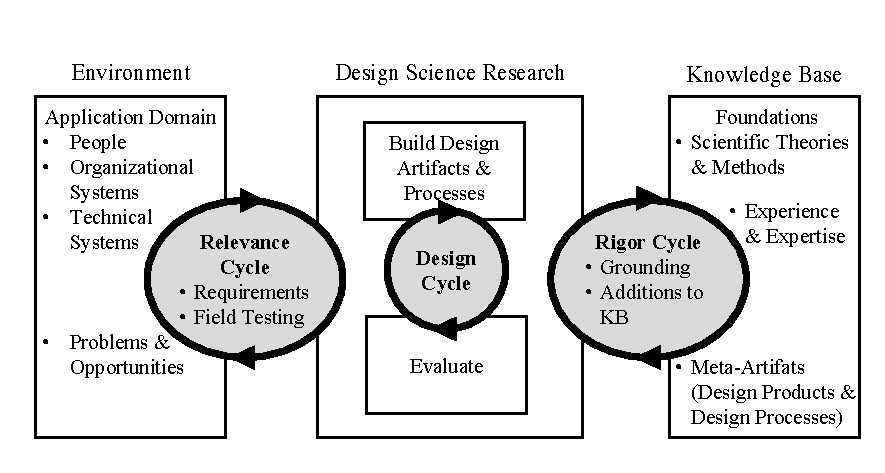
\includegraphics[width=.8\textwidth]{figures/dsr.pdf}
	} \\
\parbox{0.8\textwidth}{\quelle{\citep[\p{16}]{Hevner2010}}}
\end{figure}


\Fig \ref{fig:dsr} shows three research cycles, that should be identifiable in every \acrshort{DSR} project \citep{Hevner2010}. The environment is origin of the wish to design an artifact that solves a particular problem. In this thesis it is the absence of a process model that has referential character in the domain of \acrshort{BPO} providers in \acrshort{CRM}. The contextual environment of the partnering  \acrshort{BPO} provider is used to define requirements, which are transferred via the relevance cycle to the \acrshort{DSR} component. Its inherent design cycle brings together the building of the artifact and its evaluation. An (IT)-artifact can be a model \citep{Hevner2010} like the reference model at hand. Evaluation of the design with help of the relevance cycle ensures that the problem is addressed in a meaningful way. The design itself is connected to the knowledge base via the rigor cycle. It draws from vast knowledge in form of scientific theories or experience and expertise. It bases the design of the artifact on existing knowledge. By using proven methods and structures of reference modeling, a solid foundation is chosen. The application and transfer into the domain is supported by data from literature, as well as by qualitative research in form of interviews with experts. These two data sources are mentioned in the relevant literature \citep[\p{247}]{thomas2006mang}. The separation from routine design implies that a thorough examination is necessary in the design process to ensure the universal applicability of the reference model artifact. 


%%%%%%%%%%

%
%	\begin{tikzpicture}
%	[node distance=.5cm,
%	start chain=going below,]
%	
%	\node[punktchain, join=by {-}] (investeringer)      {Investeringsteori};
%	\node[punktchain, join=by {-}] (perfekt) {Det perfekte kapitalmarked};
%	\node[punktchain, join=by {-}, ] (emperi) {Emperi};
%	\node (asym) [punktchain ]  {Asymmetrisk information};
%	\begin{scope}[start branch=venstre,
%	%We need to redefine the join-style to have the -> turn out right
%	every join/.style={-, thick, shorten <=1pt}, ]
%	\node[punktchain, on chain=going left, join=by {-}]
%	(risiko) {Risiko og gamble};
%	\end{scope}
%	\begin{scope}[start branch=hoejre,]
%	\node (finans) [punktchain, on chain=going right] {Det finansielle system};
%	\end{scope}
%	\node[punktchain, join=by {-},] (disk) {Det imperfekte finansielle marked};
%	\node[punktchain, join=by {-},] (makro) {Investeringsmssige konsekvenser};
%		\node[punktchain, draw=pink] (aux1) { };
%	\node[punktchain, below right=0.6cm and -1.975cm of makro] (konk) {Konklusion};
%	\node[punktchain,  left = of konk,] (konk2) {Konklusi2on};
%		\node[punktchain, below= of aux1 ] (m1) {m1};
%	% Now that we have finished the main figure let us add some "after-drawings"
%	%% First, let us connect (finans) with (disk). We want it to have
%	%% square corners.
%	\draw[|-,-|,-, thick,] (finans.south) |-+(0,-1em)-| (disk.north);
%	\draw[|-,-|,-, thick,] (emperi.south) |-+(0,-1em)-| (risiko.north);
%	\draw[|-,-|,-, thick,] (emperi.south) |-+(0,-1em)-| (asym.north);
%
%\draw[|-,-|,-, thick,] (makro.south) |-+(0,-0.7em)-| (konk.north);
%\draw[|-,-|,-, thick,] (makro.south) |-+(0,-0.7em)-| (konk2.north);
%
%\draw[|-,-|,-, thick,] (konk.south) |-+(0,-0.7em)-| (m1.north);
%\draw[|-,-|,-, thick,] (konk2.south) |-+(0,-0.7em)-| (m1.north);
%
%	% Now, let us add some braches. 
%
%	\draw[tuborg, decoration={brace}] let \p1=(perfekt.north), \p2=(emperi.south) in
%	($(2.5, \y1)$) -- ($(2.5, \y2)$) node[tubnode] {Problemfelt};
%	\end{tikzpicture}
%		
		
		
	
	%%%%%%%%%%
\section{Empirical Research}
	%%%%%%%%%%
	As stated in the epistemological positioning, a Kantianistic view with cognition from intellect and experience is taken. While the cognition from intellect is of special importance in design of the artifact, the transfer of knowledge from domain experts motivates the cognition from experience in evaluation and requirements specification. 
	%wegkopiert nach vorne
	
	The communication with the research partner was key for gaining insights into the domain. As automated process modeling approaches, like process mining, are not possible due to a lack of suitable data, manual techniques are used. These require a data basis, which builds on the school of empiricism. Qualitative research techniques in form of workshops, document analysis and interviews are used in the research project. 
	
	A plan for the selection of interview candidates was developed in collaboration with the research partner to ensure coverage of the application domain, which is a form of theoretical sampling\footnote{For more information about sampling in qualitative studies see \citep{coyne1997sampling}.}. In a top-down approach managers from core processes in the organization were interviewed face-to-face or by call. For this thesis, interviews with nine domain experts were conducted, transcribed and analyzed. Each interview lasted for \apprx 40 minutes. Additional presentations and documents were provided by the interviewees and served as an additional source of information. Since the thesis is part of an ongoing research project, other data sources that were not directly connected to the thesis are used like the outcomes of a process modeling workshop and notes from previous meetings, where no transcription is available. The process modeling workshop was conducted over two days and included four practitioners and four researchers. 
	
	Analysis of data started before all interviews were conducted, as coverage of fields of interest was necessary on the required detail level. 
	
%interviews
%data, --> ECIS paper draft. 
% analysis of papers?
	
	

		
\chapter{Research Background}
	%%%%%%%%%%
	This chapter introduces the reader to the domain and reference modeling. Special emphasis is put on the field of \acrshort{CRM} so that the author's conclusions in the modeling chapter can be followed by a solid theoretic foundation. Reference modeling as a method is presented in less extent, as it is does not contribute to the model's content matter.
	
	\section{Domain}
	%%%%%%%%%%
	In context of this work, the domain expresses the content of the reference model. This section covers \acrshort{BPO}, \acrshort{CRM} and the merge of both areas to support comprehension of model design choices.
		%%%%%%%%%%
		\subsection{Business Process Outsourcing}
		%%%%%%%%%%
		The phenomenon of outsourcing can be explained by basic economic theory. The following section describes how the theory of the firm, the value chain, outsourcing and process orientation are interwoven. 
		
		
		\subsubsection{Theory of the Firm}
		In theory, a firm exists because of transaction and production costs efficiencies. Firms are organizational innovations to reduce costs involved in market transaction. A transaction here means the transfer of a good or service across a technologically separable interface \citep{williamson1981economics, williamson1971vertical}, \eg the boundaries between firms. If the transaction costs across markets become larger than the costs of managing the firm, firms will substitute market transactions through internal execution. IT has drastically reduced these transaction costs and the IS field is applying transaction cost theory to explain its impact on the boundaries of the firm \citep{aron2005just}.
		The theory of production cost efficiency states that production by multiple individuals is the characteristic of a firm \citep{alchian1972production} and it will exist as long as the output is sufficiently larger than the output under independent production, so that the costs of organizing individuals are justified. With increasing output, economies of scale describe the positive effect on unit costs. 
		
		Productivity typically increases with specialization, which explains why firms specialize in certain tasks: costs of managing the firm increase with size, benefits in productivity are achievable through focusing on core business.
		A company can develop parts into its core business, that others do not. They can provide these as services on the market place - and decreasing transaction costs make it more and more attractive to make us of these. 
		
		\subsubsection{The Value Chain}
		Drawing on the concept of the value chain by \cite{porter1985}, the idea is to model each firm as a set of systems, which add value to a product or service. These chains can be concatenated, as more and more actors are involved on the way to the end consumer to make a final product out of raw materials and components. Transaction costs are the glue that hold chains together, because their existence links established connections.  Within each chain lie different subsystems, which contribute to the created value through the consumption of resources - like money, labor or material. Strategy demands that firms build sustainable competitive advantages to be able to survive in the market. As firms cannot build these in all stages of their value chain \citep{Ramachandran2004}, they choose to focus on certain activities (core business) and hence invest less resources in others. 
		
		As transaction costs are composed of costs for communication and information processing \citep{evansted}, one can see how digitalization impacts these theories from the last century. With communication costs dropping to nearly zero due to the internet, value chains can easier break up and be more flexible. 
		
		As a result of the combination of the aforementioned theories of the firm and the value chain, organizations are incentivized to transfer activities to other actors in the market who have specialized on them and therefore can deliver it better and more efficient.
		
		%Combining the previously mentioned theories of the firm and the value chain, organizations can easier transfer activities to other actors in the market that have specialized on it and can deliver it better and more efficient.  
		
			\subsubsection{(Business Process) Outsourcing}
			\label{sec:bpo}
		The term outsourcing can be derived from \textbf{out}side re\textbf{sourcing} and dates back to 1981\citep{oxford}. It can be broadly defined by \enquote{the purchase of a good or service that was previously provided internally} \citep[\p{74}]{lacity1993} or narrowly as \enquote{contracting with an external firm for the ongoing management and delivery of a defined set of services to a prescribed level of performance} \citep[\p{2}]{cohen2006multisourcing}. However, it does not necessarily mean relocating it to a foreign country (offshoring), which falsely gave the term a negative connotation in Germany in the past\footnote{ "Outsourcing" was chosen the Un-word of the year 1996 \url{http://www.unwortdesjahres.net/index.php?id=33}}. Outsourcing can be distinguished from other types of partnerships through a contract that clearly defines subject and duration of the cooperation \citep[\p{28}]{gross2006}. 
		
		\cite{Lee:2000} give an overview about theoretical foundations in outsourcing research. Three major views are identified:
		
		\begin{itemize}
			\item Strategic management view
			\item Economic view
			\item Social view
		\end{itemize}
		
		The first builds on the resource-based view \citep{wernerfelt1984resource} and takes a merely internal view. Here, the firm's strategy is about its capabilities, captured in scarce resources, and explains outsourcing of non-core activities to focus on its core competencies. The economic view brings transaction cost theory into play and argues that specialized organizations (outsourcing providers) are able to achieve economies of scale in producing services. Lastly, apart from this cost efficiency focus, relationships between provider and client are also an issue worth explaining. Here, social exchange and power political theory \citep{lee1999effect} can be named. This view is justified by two mechanisms that are explaining relationships between organizations, namely trust and power. These play an important role in establishing and especially maintaining a relationship, which is leveraging economies of scale and scope provided by partnering organizations \citep{rai1996critical}. Trust facilitates outsourcing by transferring responsibilities to a provider and power structures define shape of the agreement.
		
		% despite the fact that earlier work in the field \cite{cheon1995theoretical} did not consider it
		
		Processes\footnote{For sake of completing the introduction to outsourcing, processes are discussed in the next section. } in which IT plays an important role became prime candidates for outsourcing \citep[\p{27}]{gross2006}, as transaction costs for information are negligible. More precisely, one can speak of \acrfull{ITES} that can be outsourced using the power of IT \citep[\p{49}]{Ramachandran2004}. In addition, IT itself has become the most outsourced function (60\% penetration \citep{deloitte2014outsourcing} considering firms with more than 1 billion USD revenue) and is called \acrfull{ITO}. Next to IT, finance, legal, real estate and facility management, HR and customer service are popular outsourcing applications \citep{deloitte2014outsourcing}. 
		
		\acrshort{BPO} is a special form of outsourcing. It is defined as the transfer of complete processes to an external service provider \citep{wullenweber2008impact}. \cite{mani2010emp} add that IT-enabled processes are subject to BPO. It is unquestionable that the reduction in transaction costs driven by IT enables the BPO business and that IT will expand its importance. One can argue that BPO, which requires more coordination and a more complex relationship between client and provider than outsourcing, is only possible through IT as an enabler: The transaction costs without the empowerment of IT for outsourcing complete processes are too high to be reasonable from an economic point of view. This work views  BPO as \enquote{the delegation of one or more information technology enabled processes to an external service provider} \citep[\p{39}]{mani2010emp}.
		
		\subsubsection{Process Orientation}
		\label{processorientation}
	Drawing from the  \acrfull{ARIS} \citep{Scheer1997}, one can take four different perspectives on modeling businesses from an \acrshort{IS} perspective: organizational, functional, data and process. The process perspective integrates the other three views. The concept of processes is a central part of this thesis. 

	Research revealed, there are conflicts in the wording between the business process management and outsourcing domain. A process is defined a self-contained time-logical sequence of activities that work on a business relevant object \citep[\p{6}]{becker2012pm}.
	A business process is used synonymously with a process in this work. Reason for this is that the notion of business process within BPO only stresses the outsourcing of complete processes and views every outsourced process as a business process.  An example for this conflict is that outsourcing the payroll management process would be considered \acrshort{BPO}, while the very nature of the process is clearly not directed by the business objectives of the company as the definition of business process according to \citep[\p{6}]{becker2012pm} would state. 
	
	Porter's value chain differentiates into primary and supporting activities \citep{porter1985}. The former directly contribute to the created product or service and therefore have impact on the economic outcome of the company. Porter names logistics, operations or service as parts of these primary activities\footnote{However, the differentiation in primary and supporting activities highly depends on the business of the company.}. Yet, supporting activities do not have a direct relatedness to the product or service, but are necessary to perform primary activities. Human resource management or IT can be named here. This distinction between primary and support activities may be flowing and leaves room for interpretation and is additionally dependent on the business domain and company itself. Furthermore, one can add coordinating activities to the list, as they are required in an organization. These three activities are applied to processes that shall be distinguished in core, support and coordination processes. 
	 
		\subsubsection{A Framework for BPO Participants}
		\label{sec:frameworkbpo}
	There are at least two parties involved in an outsourcing setting. The company that is outsourcing a process is called \textit{client}, while the business that is servicing the outsourced process is called \textit{provider}. This thesis focuses on building a model for the provider and takes its perspective. Due to this view, it is also referred to as the focal company. With respect to the outsourced process, additionally there may be \textit{customers} involved. These can be other businesses or private consumers.  \Fig \ref{fig:outsourcingERM} shows an \acrfull{ERM} \citep{Chen:1976:ERM} among participants.
			\begin{figure}[caption={Outsourcing ERM}, label={fig:outsourcingERM}]
		{	\includegraphics[width=.8\textwidth]{figures/outsourcingERM.pdf}}
	\end{figure}
	
	Client and provider are connected through their outsourcing agreement and a provider is very likely to have multiple of these relationships. Multi-Sourcing, \ie, the outsourcing of services to multiple providers even within a functional area is reflected in the \textit{(1,n)} relation of the client to the provider. Clients and their customers are connected, as a customer is buying goods from multiple companies (clients), which in turn have multiple customers. The outsourced process can involve client customer contact (for instance in CRM), but does not have to (accounts payable). In addition, a customer may be connected to multiple outsourcing services and every outsourcing service is likely to handle multiple client customers. 
	
	The outsourcing of customer facing processes is often not to the knowledge of the customer \todo{src}. This is due to the fact that clients do not have interest in confusing their customers or weakening their brand by bringing another party into their relationship with the customer. Hence, client and provider fuse to one unit from the customer's perspective (one face to the customer policy). \Fig \ref{fig:bpochain} visualizes the described B2B2B/C chain as an analogy on B2B and B2C as existing shorthands for business-to-business and business-to-consumer. The chain underlines the two critical intersections of the focal company (provider) with the other markets. As shown in the ERM, an outsourcing provider has multiple clients (each having customers that may be part of the outsourcing) and hence provider's businesses can be visualized as multiple chains with different client and customers attached to the provider. Consequently, these form markets that the provider interacts with.
	
		\begin{figure}[caption={BPO B2B2B/C Chain}, label={fig:bpochain}]
	{	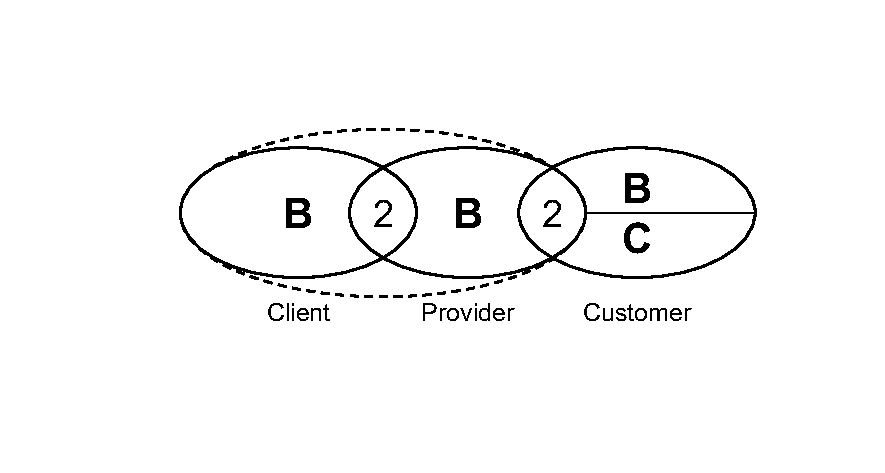
\includegraphics[width=.8\textwidth]{figures/bpochain.pdf}}
	\end{figure}

		\subsubsection{Outsourcing Client}
		%% irgendwie wiederkehrende Struktur bei Parent Company und Provider...
		Motivation for outsourcing of services is based on sound economic principles, as laid out in the section on theory of the firm. From the previously described theories, especially the economic and strategic management view applies to the justification of outsourcing decisions. \citeauthor{bartell1998information} names improved business focus, mitigate risks, build sustainable competitive advantage, extend technical capabilities and free resources for core business purposes \citep{bartell1998information}. Cost reduction is not included in this list (even though it was a primary driver at first), as the experience has shown that 80\% of customer service outsourcing projects aimed for cost-cutting are failing to meet their goals\footnote{\cf \url{http://www.gartner.com/newsroom/id/492113}}. \citeauthor{gross2006} name cost savings, quality improvements and increase in capacity \citep[\p{77}]{gross2006} as reasons for \acrshort{BPO}. 
		\todo{gross nennt 3 gründe (77))+ beispiele mit customer service. }
		\todo{cost savings argument noch diskutieren, zahlen von schewe, auch bei gross}
	
		\subsubsection{Outsourcing Provider}
		
		The business of an outsourcing provider is oriented towards clients. Outsourcing contracts are individually negotiated and can put the provider into different roles. While companies can use outsourcing as a means to drop off operative work and manage related processes by themselves, a closer relationship between provider and client facilitates more cooperation. Providers can become partners that take responsibilities collateral to their front-line business. 
		
		\cite{schewe2007} provide a framework for processes of an outsourcing provider, which is located in Appendix \ref{app:provproc}. It counts three main areas: service management, delivery management and service delivery. Service management comprises \textit{client support} and \textit{help desk}, which are about maintaining the client relationship and providing help with respect to the provided services, respectively. Delivery management can be loosely compared to product development in a manufacturing business. It contains \textit{program management}, which handles the offered service portfolio and \textit{projects}, that develops and deploys new outsourcing engagements. The last area, service delivery, is about the outsourcing activity itself. Its components are \textit{finance}, \textit{HR} and \textit{procurement / logistics}, as well as \textit{transaction processing}. The latter refers to the creation of services, which is the main business, while the first three are supporting activities for service delivery. 
			
		A recent market overview segments BPO-providers into five categories: \acrfull{HRO} specialists, customer care specialists, BPO multi's, IT multi's and document management providers \citep{hfs2016top}.  While the authors note that the split is subjective, it helps to get an overview about the market's composition, as shown in \Fig \ref{fig:bpomarket}. The notion of customer care is hardly seen in academics, as a search on sciencedirect unveils\footnote{1294 results for \enquote{customer service} in title, abstract or keywords in comparison to 58 for \enquote{customer care}}. It seems that customer care is used to emphasize activities that exceed narrow customer service provision. Here, the term \acrshort{CRM} is preferred to capture this extension, which is reasoned in the following.	
			
		\begin{figure}[caption={BPO Market Composition}, label={fig:bpomarket}]
			{
				\begin{subfigure}[b]{0.45\textwidth}
					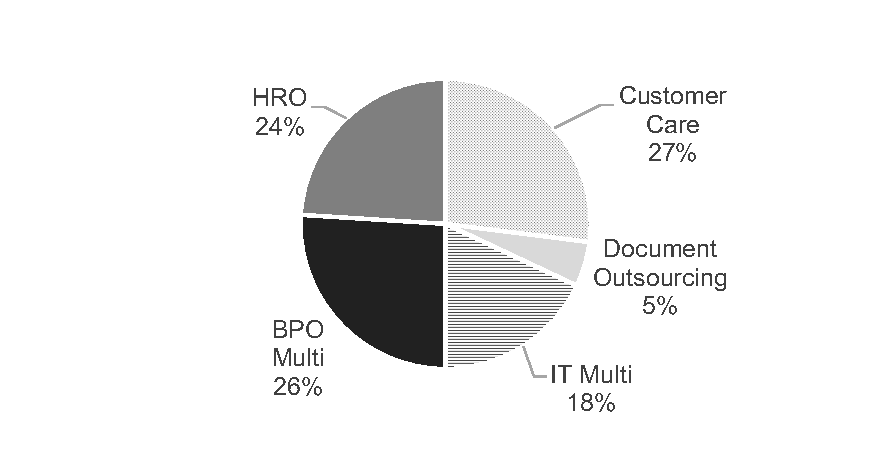
\includegraphics[width=.8\textwidth]{figures/bpomarket.pdf}
				\end{subfigure}
			\begin{subfigure}[b]{0.45\textwidth}
				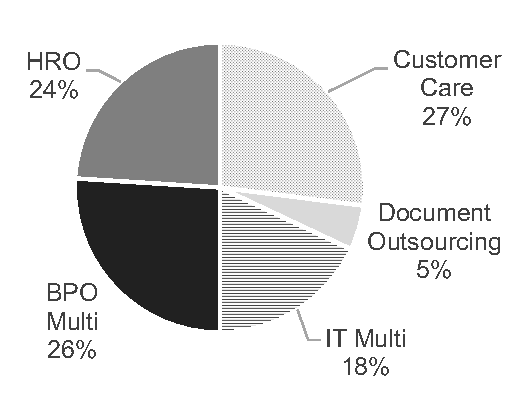
\includegraphics[width=.8\textwidth]{figures/bpotypes.pdf}
			\end{subfigure}
					
		 \parbox{0.8\textwidth}{	\quelle{\citep[\pp{5--6}]{hfs2016top}}} }
			
		\end{figure}

		In terms of growth, customer care is expected to grow 4\%, which is one percent behind the highest growth rate expected in HR providers. The \acrshort{BPO} market in general is expected to continue its increase in volume in a linear manner. 
		%%%%%%%%%%
		\subsection{Customer Relationship Management}
		%%%%%%%%%
		\label{sec:crm}
		\enquote{A company's most precious asset is its relationship with its customers} is a quote of Theodore Levitt, Harvard Business School professor emeritus \citep{levitt1983}. Following this idea, marketing has undergone a shift from a brand- or product-centricity to a more customer-centered view \citep{Chen_2003}. An absence of sharp definitions has led to a considerable confusion in academic literature about the term customer relationship management \citep{paynefrow2005}. 
		
		Essential terms surrounding CRM are marketing, relationship management and relationship marketing. Drawing on the taxonomy of \cite{Leuer2011}, a visualization of the fundamental relationships is given in \Fig \ref{fig:crmcircles}. Under the umbrella of marketing, relationship management describes the active and systematic analysis, planning, design, selection and control of all business relationships in the sense of a holistic concept of systems, activities and goals \citep[\p{442}]{diller1995}. It has to be noted that not only relationship to customers, but also suppliers, communities, authorities as well as internal relationship are enclosed by this term. Relationship marketing is a subset of relationship management and more strongly emphasizes customers as a target, but also comprises vertical relationships, i.e., relationships to suppliers. Within relationship marketing lies customer management or customer relationship management. Both terms are often used interchangeably  \citep{Leuer2011,ryals2001customer}. Conducting an analysis of publications \wrt the terms, \acrshort{CRM} is identified as the most used term (\cf Appendix \ref{app:mcoc}). Therefore, this thesis prefers the term customer relationship management.
		
		\begin{figure}[caption={CRM in the Field of Marketing}, label={fig:crmcircles}]
			{	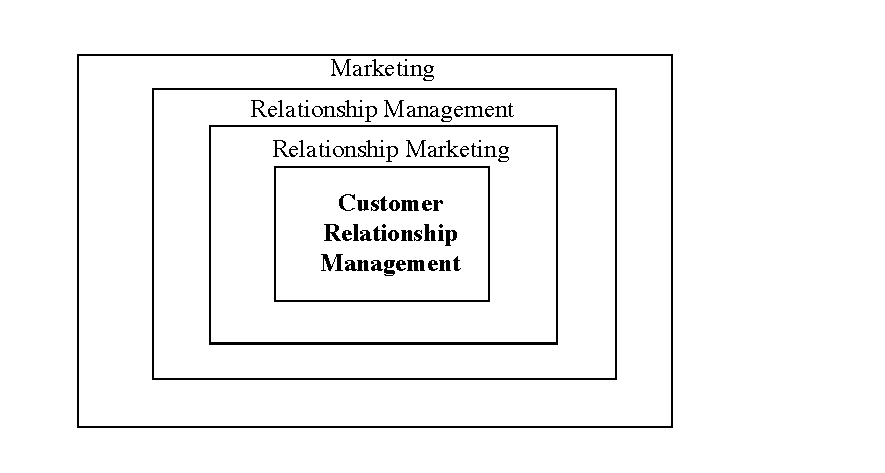
\includegraphics[width=.8\textwidth]{figures/crmcircles.pdf}}
		\end{figure}
	
		\citeauthor{Chen_2003} see a process, people and technology component in \acrshort{CRM} \citep{Chen_2003}. \cite{paynefrow2005} compile different standpoints and propose three views that will be described in the following. As the name suggests, the building and sustaining of relationships to customers is always a defining characteristic of \acrshort{CRM}, but the importance of the technological component is varying. 
		
		Narrowly and tactically defined, \acrshort{CRM} refers to a technology solution and its implementation, which justifies the term's popularity in the technical field to create one view of the customer in the \acrshort{IS}. With an increased scope, \acrshort{CRM} can be seen as the implementation of an integrated series of customer-oriented technology solutions. Widely and strategically defined, \acrshort{CRM} can be seen as a holistic approach to managing customer relationships to maximize customer value, corporate profitability, and thus, shareholder value \citep{payne2004role}. This value is realized through the developed of a relationship that is profitable and preferably long-term.  Customer service is seen as part of \acrshort{CRM} \citep[\p{11}]{Helmke_2012}. It exists in order to create additional value before, during and after a purchase. 
	
		For this thesis, a customer is defined as an individual or business that has entered the process of buying a good or service from another business. Hence, the customer has a relation to the latter that is of interest in CRM. This relationship can be strengthened by a plethora of marketing instruments that businesses use to bind the customer. These are initiated from the businesses and directed towards the customer. The reverse way, \ie, a customer reaching to the company by considering a product is also possible. 
		
			\begin{figure}[caption={CRM Processes}, label={fig:crmprocessfr}]
			{	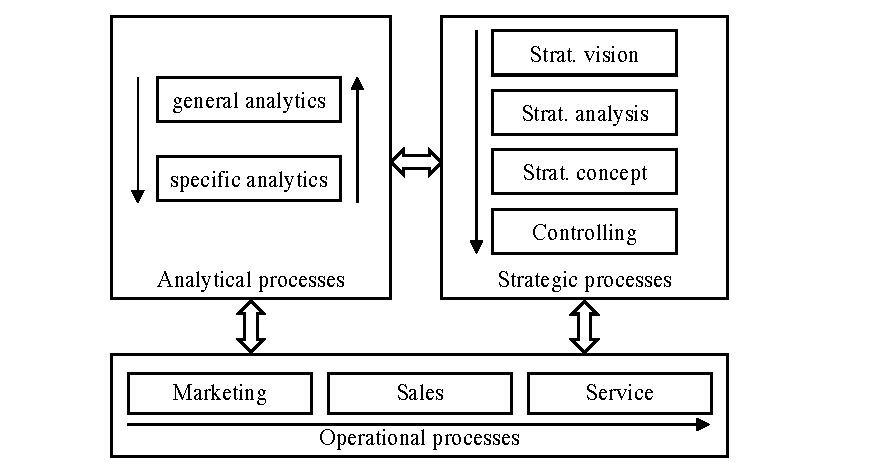
\includegraphics[width=.8\textwidth]{figures/crmprocessfr.pdf}	
	\\
						 \parbox{0.53\textwidth}{\quelle{adapted from \citep[\p{39}]{Helmke_2012}}}
			 } 

		\end{figure}
	
		
		Processes in CRM can be divided into strategic, analytical and operative \citep{Neckel2005}. Strategic processes build up on an strategic analysis (for instance \acrshort{SWOT}) to derive goals of the CRM initiative and structures necessary to reach them. Operative processes describe execution loosely separated in marketing, sales and service processes. Analytical processes support both strategic and operative processes through data-driven insights either on a general level (\ie, customer segmentation) or bound to a specific activity (\ie, cross-selling). Operative processes are customer-facing processes and are of special interest to this thesis. 
		
		 For contact between the company and customer, two terms have emerged: (interaction) channels and customer touch points \citep{Leuer2011}. A channel is a medium that facilitates communication and is seen from a company perspective, while a customer touch point is more specific and from the customer's point of view. A touch point shall be every moment of contact with the company from the customer's perspective \citep{Zomerdijk_2010}. Linking touch points together forms a customer journey. 
		 
		 A channel can be composed of platforms. Social media as a channel represents platforms like facebook, twitter or instagram. Channels are likely to be a long-lasting media in CRM, while a platform may or may not withstand the test of time. In social media, platform members can publicly communicate via posts, which are touch points between company and customer. 
		 However, it is noted that one can see platforms as separate channels in business, as they require different handling in operations. This granularity stands in contrast to the intended applicability of this work, therefore social media platforms are not treated separately. 
		
		Communication between the customer and company can be done through a number of channels which have grown in the past years. Integration of these channels is a central task of CRM and shows increasing complexity. \cite{paynefrow2005} propose six categories: (1) sales force, (2) outlets,\ie, stores and the alike, (3) telephony, (4) direct marketing,\ie , mail, radio, television, (5) e-commerce,\ie , email and internet, (6) mobile-commerce (\ie, text messaging, mobile telephony). Applying the \acrfull{MECE} rule, one faces problems with this definition. With the advent of smart phones, mutually exclusion of (3), (5) and (6) is hardly possible. In addition, social networks have become increasingly important for customer interaction. This necessitates another view, which adequately represents today's channel landscape and is forearmed for new channels that might emerge in the future. 
		
		This thesis takes a two-dimensional view on different interaction channels in CRM that defines four quadrants. Building on the framework by \cite{paynefrow2005}, the digital component gets more emphasis, as it is of striking importance today. The matrix displayed in \Fig \ref{fig:channelmatrix} positions different channels with respect to their personal or universal way of communication, as well as their orientation towards IT. The aforementioned categories (1) sales force, (2) outlets and (4) direct marketing are located in the matrix with no further change of meaning to the primary literature. Especially in the digital sphere, a more diverse view on the remaining problematic categories is taken. The channels in scope are described in the following section. 
		
			\begin{figure}[caption={Channel Matrix}, label={fig:channelmatrix}]
			{	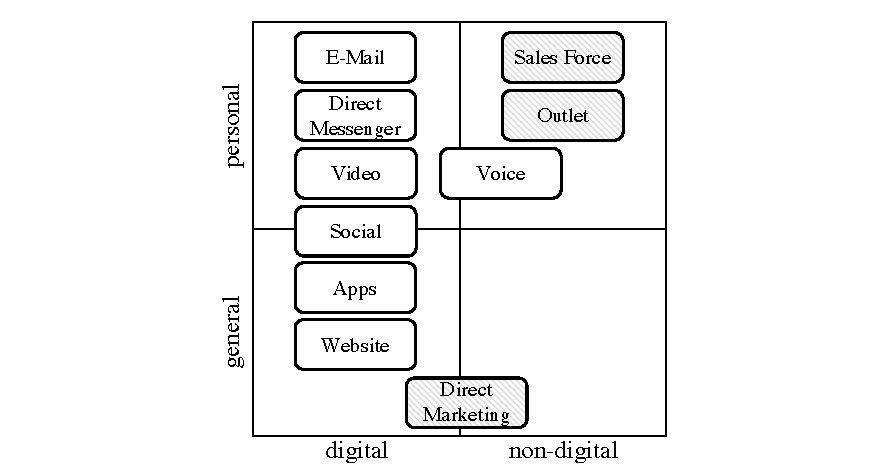
\includegraphics[width=.8\textwidth]{figures/channelmatrix.pdf}}
		\end{figure}
		
		Digital channels are characterized by the web as underlying technology for communication. Non-digital channels, however, rely on physical interaction in a broader sense. In general, a shift towards digital channels is undeniable. For customers, they are a convenient way of communication, as their devices enable them to interact with less effort. A stop at a retail store is more effortful than a lookup of information on the company website. Nevertheless, non-digital channels will always be part of the channel portfolio, as complicated issues may require interaction with another human being face-to-face, especially in the B2B-sphere. 
		
		The customer-centric view underlines the shift to personal marketing activities \citep{peppers}. This is enabled by IT and the ever increasing amount of data that is available and attributable to a single consumer. While the more personal approach is standard practice in B2B-relationships, mass media direct marketing has been the only way to target private customers in the past decades through the use of radio or television. In a data-driven world, personalized relationships with customers are an imperative to stay competitive. However, an anonymous way of retrieving information is also demanded, even though this way will likely increase the effort due to a less tailored presentation of information. This is contrary to the wish of integrating as much customer information as possible, to create a so called 360-degree view of the customer. Identification of customers for integration purposes is a key challenge there. 
		
		The two trends in the dimensions render the personal / digital quadrant as a strategic priority.
		The identification of single customers is of paramount interest for a customer-centric view, which is only possible through use of \acrshort{IT}.  
		This again can be mapped back to the work of \cite{paynefrow2005}: They name information management and multichannel integration as strategic processes. 
		
		Not every channel is used by every company, but companies tend to create multi-channel instead of single-channel strategies \citep{Frow_2007}. Coming from a pre-digital age, digital channels were integrated gradually and often in a heterogeneous information system landscape \citep{Chen_2003}. The following paragraphs shortly describe all channel categories that are not named  in  \cite{paynefrow2005}. A special focus is set on the role of customer service provision. 
		
		
		\subsubsection{Voice}
		
		Coming from traditional, non-digital telephony, voice is a very important service channel. While non-voice channels are said to overtake by the end of 2016, it is still accounting for half of the customer service volume on its own \citep{dimensiondata2016}. However, voice is becoming more and more digital for example through \acrfull{VOIP} technology, which is one reason for the renaming. Defining characteristic is the synchronous communication and interaction with a \acrfull{CSR}. A channel's popularity is reasoned by customers' expectation to explain their problem easily (35.2\%) and get a fast response (46.4\%) according to \cite{Agnischock2015}. Voice is well suited here, but is also a costly option for customer service, due to the one-to-one interaction. \acrshort{CSR}s are not able to process multiple calls simultaneously. Outsourcing call centers has therefore become a major application across industries as low-wage countries like India offer significant cost-saving potentials. \todo{common language?} 
		
		Regarding data, the shift towards digital call processing enabled the tracking of numbers, efficient routing and conversation recording for instance. Identification of callers is often possible through the caller's phone number (if not suppressed). %, but a problem arises in outsourcing: When the client provides call routing systems and uses outsourcing as a means to process first level support for instance, the phone number might not reach the provider's systems. This renders a customer identification before start of the call impossible. 
		Audio recordings are on the rise \citep{ccnet2016} also need to be automatically transformed into a processable format through sophisticated text-to-speech tools before using them for analytical purposes. Due to privacy reasons, these activities are restricted in many countries. 
		
		\subsubsection{Email}
		
		By 2020, 50\% of the world's population is expected to have an email address \citep{radicati2016}. In the developed world this number will be significantly higher. The convenience of electronic mail is the asynchronous communication from various devices, with attachments, at any time of the day and without the need to personally interact with the receiver. In customer service it is ranked second in terms of volume. 90.1\% of call centers support email \citep{dimensiondata2016} today. %Traditional mail or fax is included in this category, as it is plays an subordinate role: 1.4\% of customers call it their preferred channel \citep{Agnischock2015}. It also offers significant obstacles for customers through its slowness, costs and effort of creation and sending. 
		
		As the message content is directly processable, analytical support plays an important role in routing mails. The sender can be identified by the address that can not be suppressed. 
		\subsubsection{Direct Messenger}
		The vast adoption of smart phones replaced the temporarily very popular short messaging service (SMS) in a scratch.  While in 2012, traditional text messaging in Germany counted 162 million messages (the messenger WhatsApp: 20 million), WhatsApp overtook in 2013 and is now the goliath (667 million messages expected for 2015) in this business (39 million SMS are expected)\footnote{\cf https://de.statista.com/statistik/daten/studie/3624/umfrage/entwicklung- der-anzahl-gesendeter-sms--mms-nachrichten-seit-1999/}. The popularity stems from no character limit, no extra data plan costs and easy sharing of photos and videos. Strong network effects tie users to the platform. However, other players are existing in the market. In addition to this mobile app bound instances of messengers, many other platforms provide a direct messaging function, which is often called chat. In contact centers, the integration of a chat capability is ranked first in new investments \citep{ccnet2016}. Being a asynchronous channel from a technological perspective, it is de facto synchronous: customers expect a flowing conversation and hence a quick solution to their problems. A significant number of websites today have a chat embedded to quickly solve issues that arise while browsing. An economic advantage for messengers in customer service is that an agent is able to process multiple chats in parallel, which is not possible in voice for example. In addition, automation technology enables artificial intelligence to participate in chats. Being fed and trained by a knowledge base, so called \textit{Chat Bots} are able to dynamically infer queries from customers that are transferred via chat messages. These aspects are discussed in context of self-service technology in \ref{sec:ss}.%While complete control of bots is likely in future, support of human agents through analysis of chat input and recommending answer content contains less risk, as a human only gets decision support and still makes the decision.   \todo{same software necessary?}
		
		\subsubsection{Video}
		Video shares several characteristics with voice: It is synchronous, two human beings are involved and the communication is based on a common spoken language. In some sense, it is \textit{voice+}, as it adds the visual representation of communication partners, which is why one can argue that they will ultimately merge into one channel category. The reason for the split here is that voice has its roots in the non-digital world, while video is clearly a digital channel. In terms of adoption, voice is accepted and used across the technological, cultural and demographical sphere. This is not the case for video-based communication technology. While technological requirements (\ie mobile devices with front-cameras)  are given, it can be put into the early adopters group \wrt theory of diffusion of innovations \citep{rogers2010diffusion}. Consequently, the use in customer service is seen on the lowest ranks \citep{DimensionData2015}.  Furthermore, it necessitates the customer to use a specific software (\eg, Skype, Apple FaceTime) to get in contact, if the solution is not integrated in the browser or an app. However, it offers advantages not possible via voice for example through the ability to perform legally binding identification or show objects of interest live during the conversation. These innovations are reasons to put it into place in customer service, as the customer knows of their necessity in the process. The technology acceptance model \citep{Adams_1992} helps to explain the obstacles: customers do not see the added value in revealing themselves visually in front of a stranger and also expect it to be more complicated than a normal phone call. 
		
		\subsubsection{Social Media}
		
		More than 40\% of Germans are members of a social network\footnote{\cf \url{https://www.statista.com/statistics/312918/social-network-penetration-in-germany/}}. The dominant player on this market in the western hemisphere is facebook. Characteristics of this platform are personal profiles and the ability to interact with one network through public or private communication. Public communication is referred to as a post. With increasing adoption, companies realized the potential in \acrshort{CRM} through these platforms. The ability to communicate \textit{with} the company on a public stage in the network is a novelty, which justifies its attractiveness for customers and companies. In customer service, it is often used as a channel for complaints, as publicly sharing one's anger puts more pressure on the company and hence increases the chances of a customer to get a satisfying solution or compensation. The company needs to react quickly and well-considered to these inquiries, as the nature of social networks make it possible to generate a myriad of displeasing content by a single post (so called \textit{shit storms}). Furthermore, the answering agent represents the whole company as a single person in the post, which necessitates a review process. 
		
		The public posting also has implications on the ability to process customer inquiries. As personal or order related data should not be available on the network due to data privacy regulations, agents often have to switch to a private channel (\eg, private messenger within the platform or another channel). Despite the use in customer service, companies also use social networks as a marketing channel. As typically all published content can be commented by users, there is no clear boundary between service and marketing activities. 
		
		
		\subsubsection{Website}
		
		A company's website is likely the first address a customer visits to satisfy his information needs. It can be a starting point for switching to another channel, \ie, visiting the website for retrieving the service hotline number, or the channel that solves the problem. 15.1\% name it as their preferred contact channel \citep{Agnischock2015}. Often, a \acrfull{FAQ} section is provided to quickly answer questions in-demand. In addition to these sections, websites can offer a customer service area, that aims to solve customer problems without personal interaction of a \acrshort{CSR}, which are called self-services. 
			
		\subsubsection{App}
		Driven by ecosystems around smart phone operating systems (namely Android and iOS), small applications (apps) have emerged and enable diverse use cases for mobile devices. Companies publish their own apps to accompany products or services by additional information or functionality, which intensifies the relationship to the customer and increasingly becomes core part of value propositions. Airlines for instance offer check-in over their app to avoid queues and counters, owners of a Tesla can \enquote{summon} their car over the app to their location\footnote{\cf \url{https://www.tesla.com/en_EU/blog/summon-your-tesla-your-phone} } and home automation enables customers to control their lights. Companies benefit from access to a plethora of personal data, as the application needs to be installed on the device. In terms of customer service, the app can be seen as a gateway to other channels, as a chat can be provided, website content can be displayed or contact information for email or telephone can be shown. The development of smart, connected devices \citep{PorterHeppelmann15hbr} in connection with servitization \citep{servitization} will position apps as a focal point in customer experience and consequently as a means for customer service. 
		
		\subsubsection{Non-Digital Channels}
		While digital channels continue to grow, other ways of contact exist. For customer service, the importance is diminishable if one counts voice as a digital channel: mail and fax account for 1.4\% across age groups \citep{Agnischock2015}, with the highest popularity among the elderly. These can be included in the email channel, as their content can be digitized (\viz scanned). Brick and mortar stores, if available, amount for 28.5\% and are therefore very important. Narrowing the scope to \acrshort{ITES} leads to an exclusion of sales force or branches, as these are not outsourced. 
		
	
	\subsubsection{Self-Services}
	\label{sec:ss}
		Self-service technologies\footnote{In the following, Self-service technology and self-services are used synonymously.} enable customers to produce services without direct involvement of a service employee \citep{meuter2000self}. This automation relies on information technology to enable its functionality. Early examples include ATMs or balance checks on cellphones, which underline the diversity of self-service channel opportunities. Today, companies create comprehensive \enquote{web-based customer support self-services} \citep{Thomas:2009}, which are accessible through websites or apps. However, these examples convey that self-service technologies cannot be seen as a channel, but as an additional component that enables service delivery standalone or combined with other services. Other mixed forms of self-service with involvement of a \acrshort{CSR} \citep{Globerson_1991}  are not seen as self-service here. Solely the interaction of the self-service system with the customer is meant.
		
		Standalone self-services provide a solution to a customer's problem, \ie, by providing the needed information in a \acrshort{FAQ} section, also called self-help \citep{meuter2000self}. The magnitude of these areas is varying largely by industry and company, as it is the company's own responsibility to design, implement and maintain it. A social network component can be seen in communities or bulletin boards \citep{Thomas:2009}, where customers help themselves. These brand communities \citep{Hsieh_2017} are typically moderated by \acrshort{CSR}s to ensure correctness of solutions. Elements of gamification give incentives to participate and follow the rules. This type of crowd-sourced knowledge substitutes \acrshort{CSR}s with other customers.
		
		Company websites may be platform for advanced self-service technology that actively processes queries against a knowledge base. Chat functionality can accompany the customer service area to give a medium to communicate issues in natural language, without the need to navigate through the website. 
		
		%Additional possibilities are the support in another service process, for example through call routing automation to the correct specialist in a call center. Here, the customer receives self-services by passing information to a technological interface, which in turn determines the contact person that solves his problem.  
		
		Reasons for self-service implementation are cost savings, due to less labor-intensity and more productivity and scalability, as no employee needs to deal with the request \citep{Walker_2002, Walker_2003}. Customers can ignore service times, benefit from extended services, greater convenience and control, potentially more reliable information delivery and help themselves without the need to explain their issue to another person. \citeauthor{Blut_2016} provide a comprehensive study about technology acceptance in self-service technologies \citep{Blut_2016}. 
		
	\subsubsection{Multi-Channel and Omni-Channel CRM}
		An explosion in touch points \citep{Lemon_2016}, especially in digital media, has led to new developments in customer relationship management. Companies seek to make use of data to enhance their customer relationships and improve customer experience across and within channels \citep{Frow_2007}. However, the integration of data from various channels is a major challenge. 
		
		In the last century, \citeauthor{gilmore1998} claimed customer experience will be the next \enquote{competitive battleground}, which now seems to come into reality. A recent study named customer experience the number one priority of executives in the next months \citep{accenture2015}. For this work, customer experience shall be defined as the internal and subjective response customers have to any contact (direct or indirect) with a company \citep{meyer2007customer}\footnote{\cf \cite{Lemon_2016} for a detailed discussion of customer experience and the customer journey }.
		
		Drawing on the five strategic processes in \acrshort{CRM} \citep{payne2004role}, especially the multi-channel integration process and information management process are of special importance in this context. The former underlines the strategic role of integration from a customer experience perspective and the latter emphasizes the IT focus of CRM. 
		
		Two developments take place, multi-channel and omni-channel management. It is abstracting from the CRM case to include other domains, like retail. While multi-channel management is existing longer in the literature\footnote{For an overview of existing research see \citep{Neslin_2009}} and is now interpreted as the management of multiple channels to deliver high service quality in each of them, the notion of omni-channel management has recently emerged and seeks to deliver a seamless customer experience across channels. Omni-channel CRM originates in the domain of retail \citep{Brynjolfsson20131, rigby2011, Piotrowicz_2014} and envisioned shopping of goods across different sales channels (\ie, online, store, telehone). This concept is now transferred from goods to the customer experience in its center, so that omni-channel management creates one view \textit{of} a customer and thereby strengthens the relationship and increases its value. Measures like the customer lifetime value preferred over value creation emphasize the long-term view of the customer \citep{Lemon_2016} and the need of CRM to run like a golden thread through different interactions of the customer. A discussion towards the separation of both terms is included in Appendix \ref{app:mcoc2}.
		
	 This work agrees with the view that omni-channel management puts in a holistic view and emphasizes communication with the brand across channels. The objectives of omni-channel management emphasize the overall, holistic customer experience, which forges a bridge to the \acrshort{CRM} domain. Adding the temporal dimension of the customer relationship, these experiences over different interactions (in separate, integrated channels) describe omni-channel \acrshort{CRM} as a means for a superior customer value creation. 
	 
	
		%%%%%%%%%%
		\subsection{Customer Relationship Management Business Process Outsourcing Providers}
		\label{sec:bpocrmis}
		%%%%%%%%%%
		Putting together the theory of business process outsourcing, customer relationship management and recent omni-channel approaches, this section underlines how these concepts work together in business. 
		
		From the process groups in \acrshort{CRM}, primarily operational services are subject to outsourcing activities. Reasons for this lie in high labor intensity in customer service activities. According to a study by \cite{Aksin_2009} staff members for voice amount to 60-80\% of the overall operating budget. While strategic or analytical processes are more connected to high skilled and differentiating activities for a company, customer service includes several tasks that can be learned quickly. Outsourcing these activities makes use of (global) pay gaps and helps to realize cost savings. As the complexity of relationship management increases with the number of channels, companies find it harder to keep pace with their competitors. In addition, customers expect an individual and customized treatment, which justifies sophisticated techniques by companies to accompany them on their customer journey. Consequently, BPO providers have expanded their tool set to provide solutions for challenges in the other processes of CRM, namely strategy and analytics, instead of solely providing isolated activities (as an extended work bench).
		
		\cite{Ramachandran2004} name two capabilities of outsourcing providers. On the one hand, they intend to understand the client needs in the domain and business (\eg, CRM). This expertise is manifested in the understanding of the client's customer, as the relationship of the client to the customer is subject of the outsourcing engagement and is called the business development capability. On the other hand, the provider needs to have capabilities to execute the services efficiently. Economies of scale and scope have realized by the provider to reach a competitive cost level and superior service, respectively, which are denoted as the operational capability.
		
		As visualized in  \ref{sec:frameworkbpo} \Fig \ref{fig:bpochain}, outsourcing provider and client can form one unit when an end customer is involved in the outsourced business. Customers do not need to be aware of the outsourcing contract and therefore the customer service provision should keep up this delusion\todo{src: kunde will nicht im outgesourcten call center landen}. For instance, a \acrshort{CSR} in an outsourced setting will answer the phone on behalf of the client and does not leave any clues about being an employee of the outsourcing provider. As nowadays multiple channels are the norm, companies may outsource a subset of them, outsource all to one provider or cooperate with multiple providers (so called multi-vendor relationships) \citep{lee2009multi}. Implications on providers arise when managing more than one channel, as the aforementioned multi- or omni-channel management approaches apply. This development requires more expertise from the provider and moves away from the extended work bench analogy. The spanning of an outsourcing business across channels requires higher emphasis on information management and therefore the \acrshort{IS} landscape. Technological parameters can partly be set by the client, be it back-office systems or knowledge bases, as well as application systems that manage specific channels. Varying requirements and leeway make general statements about the provider's responsibilities vague. 
		
		Another dimension is the complexity of requests, which are outsourced. One typically differentiates in separate tiers in a contact center\footnote{The term contact center or service center is preferred over call center, as nowadays more than calls are handled in these facilities.},  that order the complexity of inquiries. Tier 1 support solves the most basic queries and is typically the first personal contact in a service inquiry. Tier 2 support handles complex issues, where tier 1 support is not able to solve the problem. Consequently, tier 2 \acrshort{CSR}s need to be more skilled and trained than tier 1  \acrshort{CSR}s. This reasons why tier 1 customer service is the first outsourcing candidate (54\% tier 1 against 37\% tier 2 outsourcing \citep{deloitte2014outsourcing}): it is more labor intensive through its gate-keeping property and requires less training to be productive in the job. There can be more than two tiers \citep{Thomas:2009} that each escalate to the next higher level.
		
		In terms of \acrshort{IS} landscape, providers have to manage a plethora of customer service systems, as clients may bring in their own. In addition, they outsource single or multiple contact channels. Their own landscape may consist of a single system in the best case, but due to a gradual introduction of digital channels, multiple systems are more likely. If new systems are put in place, clients may inherit the selection process, as the investment outlasts a typical outsourcing contract. Vendors on the market offer solutions for single or multiple channels and a provider selects the appropriate system for the client problem. Putting it into perspective across client businesses, the system landscape that the provider has to interact with can be described as highly heterogeneous \citep[\p{47}]{gross2006}, which is a reason why a centralized organization is hardly achievable. 
	
	%%%%%%%%%%
	\section{Reference Modeling}
	\label{sec:03_refmod}
	%%%%%%%%%%
	This second part of the background chapter outlines reference modeling as a method for building a model that represents businesses in a certain domain. Its concept and benefits are highlighted, and icebricks as a means for process modeling is presented along with guidelines to assess model quality. 
	
%Conceptual models are representations of an application domain used to capture the important features to be incorporated into a specific information system (Batani et al. 1992; Bodart et al. 2001). --37 vom brocke


		\subsection{Concept}
		
		Reference Models can be seen as theory of information systems \citep{Schutte1998}. Purpose of this section is to illustrate the ideas behind and intention of reference modeling.  
		
		\subsubsection{The Model as a Construct}
		
		
		A model itself is defined as an \enquote{immaterial representation of an original for the purposes of a subject} \citep[\p{1}]{BeckerGOM2012}. Based on the work of \cite{Stachowiak1973}, three characteristics of models are identified: mapping, reduction and pragmatism. Mapping describes the representation of natural or artificial originals, which can be models themselves. Reduction underlines the omission of certain elements of the original in a model. Pragmatism means that the selection of parts of the original is dependent on the intent of the model. Based on this notion, models of information systems (or information models in short) are explicit models that have information systems as subject matter. The purpose of modeling can be the constitution of application systems or the organization \citep[\p {59}]{Rosemann2012proc}. The latter is in focus here and encompasses among other aspects knowledge management, documentation of the organization and process management. Information modeling, the act of creating these models of \acrshort{IS} is a complex task, which is why reference models are a useful means to reduce this effort \citep{Becker2007} to create application models.
		 
			\subsubsection{Reference Models and Application Models}
			An information model can be specified towards a certain company, which is here denoted as an application model. Reference models, however, are not firm-specific and as the name suggests provide guidance in a defined modeling scenario. There is no accepted definition of reference model in the literature. \citeauthor{thomas2006a} compiles various definitions for reference models \citep{thomas2006a}. \citeauthor{vom2006reusable} bring in the notion of reusable conceptual models, where conceptual models are the representations of an application domain used to capture the important features to be incorporated in a specific information system \citep[\p {584}]{vom2006reusable}, as the term reference model is predominantly used in the German literature. In this work, it is agreed that a reference or application model of German understanding is a conceptual model. However it is refrained to use the terms reference conceptual model and application conceptual model over \acrfull{RM} or \acrfull{AM}. As an conceptual model's purpose is the representation of features of an information system, it is an information model. 
			
			\cite{Schutte1998} puts \enquote{universal validity} and \enquote{recommending characteristics} as defining  for a reference model. Universal validity expresses that a reference model can only be valid for a class of companies, so that it can be used for creating application models. The recommending aspects states that a reference model should capture a wanted state, which is in the modeler's intention. These two combined enable the wanted reusability, which is planned by the modeler \citep[\p{36}]{brocke2003referenzmodellierung}. However, achieving a recommending characteristic is a subjective judgment and universal validity can always be achieved by shrinking down the target class of companies \citep{thomas2006a}. Taking the user perspective, one can identify a reference model, if it is reused, disregarding whether the modeler considered its reusability  \citep{Puster2015}. Both perspectives build the working definition for this work. A reference model is defined as an information model with content that is intended to be reused in the construction of other application models. The relationship between a reference and application model is characterized by utilization of reference model components in application model construction. 
			
			The other option, namely encompassing a large target class of companies to create \textit{one} reference model, stands in contrast to practical use, as the creation of application models gets increasingly complicated the more general (and hence abstract and theoretical) \citep[\p{79}]{Schutte1998} the reference model is. Striking a balance between these trade-offs is known as the reference modeling dilemma \citep{delfmann2006adaptive}. 
		
			To capture the complexity in business, a data, organizational, functional or process perspective can be taken (\cf \ref{processorientation}). As only process models are subject matter in this thesis, the term process reference model is used interchangeably with reference model from here on. 

				  
				  \begin{figure}[caption={Design Process of Reusable Conceptual Models}, label={fig:refmodconst}]
				  	{	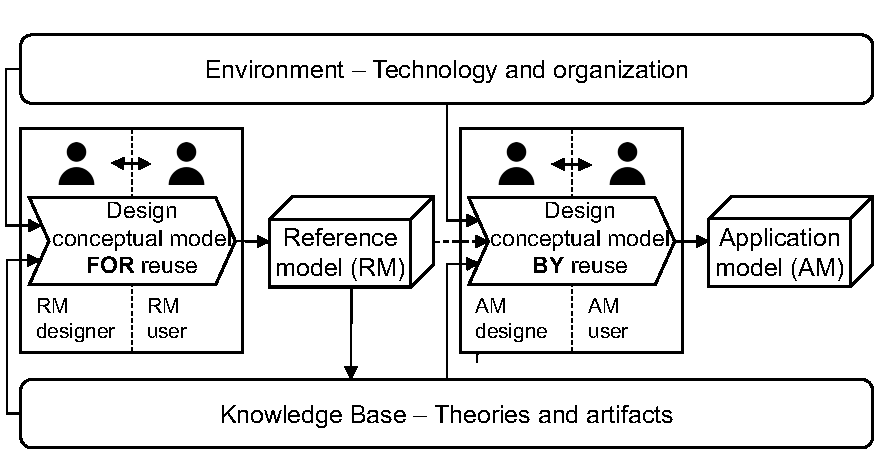
\includegraphics[width=.8\textwidth]{figures/refmodconst.pdf} \\
				  		\parbox{0.8\textwidth}{\quelle{adapted from \citep[\p{587}]{vom2006reusable}}}
				  	}
				  		
				  \end{figure} 
				  
			%grafik aus refmod - enzyklopädie vom brocke
		A model is created by one or multiple subjects called designers and utilized by users \citep{becker2004handelsinformationssysteme}. Model designers in context of reference modeling are responsible for creating the \acrshort{RM} itself. Their intention is to design \textit{for} reuse, \ie creating an artifact that is to be reused. The other involved stakeholder in this modeling process is the reference model user who collaborates with the designer and defines requirements for use. This first process is visualized in the left chevron in \Fig \ref{fig:refmodconst} and takes input from the knowledge base as well as the environment. The output is the  \acrshort{RM} which itself contributes to the knowledge base as an artifact. 
		
		The right chevron is similarly structured \wrt the stakeholders, but designs an application model on base of the now existing \acrshort{RM} which can be labeled as design \textit{by} reuse. Akin to the reference model designer, the application model designer takes requirements from the application model user. By doing this, the  \acrshort{AM} can represent characteristics of the application environment (\ie one organization), while still being conformable to the reference model. 
		
		\subsubsection{Construction}
		A construction of an \acrshort{AM} on basis of a \acrshort{RM} requires the construction of the latter beforehand. 
		\Fig \ref{fig:refmodconst} lists the knowledge base (theories and artifacts) and the environment (technology and organization) as inputs for reference modeling. For knowledge acquisition, one can differentiate in an inductive and deductive approach \citep{thomas2006mang}. Inductive conclusions  might stem from the organizational settings that are observed or existing \acrshort{AM}s of organizations in the domain. Deduction is employed when drawing on existing theories from the knowledge base. Loosely, these two approaches refer to the two inputs for design \textit{for} reuse in \Fig \ref{fig:refmodconst}. 
		
		The reader is referenced to \cite{Fettke2014meth} for an overview about different construction techniques. These show conformance with the design science approach \citep[\p{10}]{Puster2015} which is taken here. 
		
		
		\subsubsection{Selected Reference Models}
		\label{mod:scor}
		As mentioned, a reference model is suited to fit requirements of a certain domain. The purpose of this section is to briefly present two different reference models that are used in practice: The \acrfull{SCOR} Model and the Retail-H. Both show a layer structure to manage complexity and both encompass a process reference model. Figures showing the framework are located in Appendix \ref{app:refmods}.
		
		\acrshort{SCOR} allows modeling of supply chains. It is a process reference model with three detail layers. It was developed in 1996 and is now maintained by the Association for Operations Management \citep{APICS2015}. On the highest level, typically called regulatory framework, \acrshort{SCOR}  is based on six distinct management processes: Plan, Source, Make, Deliver, Return and Enable. While the regulatory framework assists in defining scope, the second configures the type of supply chain (Make-to-Order, Build-to-Order, Engineer-to-Order). On the third level these processes are decomposed into generic process steps (e.g., issue product). Even more detailed processes are considered company specific and therefore no part of the model. Furthermore, performance metrics are also defined on each level. 
	
		\label{mod:retail}
		In the domain of retail, the Retail-H is a reference model that includes process, function and data models. Developed by \cite{becker2004handelsinformationssysteme}, it has been adapted to suit special segments of the domain\footnote{for instance eCommerce, Central Clearance or Central Settlement \citep{Puster2015}}. 
		It is structured with four layers of detail: the regulatory framework, main processes, detail processes and process building blocks, as an application of icebricks as a process modeling language. The core of the regulatory framework is made up of three parts that form the H (a connection to the German word for retail: \enquote{Handel}). While the left part of the H describes the supply side, the right covers the distribution side. Both are connected through logistics. All of these core processes are business processes, the roof and foundation consist of support processes, thereby making use of the framework reference design as proposed in \cite{Meise2001}, while simultaneously capturing domain-specific aspects in the set-up of the framework.  
		
	
		

		%%%%%%%%%%

		%%%%%%%%%%
		\subsection{Benefits}
		
		\citeauthor{becker2004handelsinformationssysteme} name benefits of reference models in combination with an explorative study \citep[\pp{75}]{Schutte1998}. Similar to \cite{vom2006reusable}, they differentiate in model designers and users. Reflecting on \Fig \ref{fig:refmodconst}, actors in the left process are subject in this section. Taking the view of the two parties, the following benefits are named:
		
		\begin{itemize}
			\item Designers
			\subitem Monetization through application and configuration
			\subitem Obtaining domain knowledge
			\item Users
			\subitem Cost reduction
			\subitem Risk reduction
			\subitem Documentation
			\subitem Analysis
			\subitem Exchange of information  
		\end{itemize} 
	
		Designers of \acrshort{RM} are a research institutions or businesses. This distinction is not mutually exclusive,  but helps to conclude the two main benefits. While the economic principles encourage the monetization through the use of the \textit{product} reference model, the scientific world strives for cognition in the domain. It is noted, that the practical use of a reference model to form an application model is seen as hardly possible without additional consultative services in application model design \citep{Schutte1998}.
	
		The user side puts emphasis on cost reduction aspects \citep[\p{76}]{Schutte1998}. This stems from the avoidance of modeling from scratch which creates quality gains and time savings. Related to this, risk reduction refers to less modeling mistakes as the application model builds on a solid foundation. Through a more structured approach of information modeling, an improved documentation can be achieved. The analysis and identification of weak spots is especially important in process reference models \citep[\p{81}]{becker2004handelsinformationssysteme}. Finally, the exchange of information inside the company benefits from a common base for discussion. It can be summarized as \textit{best practice sharing}. A feedback loop from users to designers also facilitates further development and adjustment of existing \acrshort{RM} to new circumstances in the domain. \todo{vombrocke checken!}
		
		%%%%%%%%%%
		%%%%%%%%%%
		\subsection{icebricks as a Process Modeling Language}
		\label{sec:iceb}
	 A language is a system of signs and rules to their use \citep[\p{11}]{holten1999}. Fundamental is the ability to represent and communicate information through it \citep[\p{64}]{brocke2003referenzmodellierung}. While reference models are formulated in various languages, several options may arise. There are reference models like \acrshort{SCOR}, which avoid the use of a defined modeling language to ensure wide industry adoption through not interfering with used modeling languages. However, this necessitates an increased complexity in adoption, as an application within a company requires the translation into a sound process modeling language. While the framework level does not need to comply to a formalized language, more detailed layers of the reference model without clearly defined syntactical guidance increase the risk of misunderstanding among users.
	 This reasons the choice of using a defined process modeling language for this undertaking.
	 
	 The next step is to decide what language to use. Traditional modeling languages like the \acrfull{EPC} or \acrfull{BPMN} show similarities. Being syntactical languages, they offer large degrees of freedom in usage. What might look like an advantage at first sight, turns out to be disadvantageous. As process management approaches have increased number and variety of model designers and users enormously, more and more non-experts get in contact with process models and thus create models of less quality \citep{Rosemann_2006}. The definition of modeling conventions becomes necessary to help the modeler to conform certain standards. A way to confront this challenge are the \acrfull{GOM} \citep{BeckerGOM2012}, which are an analogy to the \acrfull{GAAP}. However, conforming to these guidelines will lead to increased resource requirements in these undertakings. Semantic process modeling languages avoid this by enforcing additional rules that models have to follow. Icebricks \citep{clever2016} is one example that realizes this concept and has been used for reference modeling. In addition to syntactical correctness, \ie, conforming to an existing language's meta model, other aspects are also considered which would otherwise be taken care of by combining \acrshort{GOM} and syntactical languages. Because the additional check for guideline compliance is unnecessary in semantic languages, they are more efficient. After a short summary of the language,  the \acrshort{GOM} are described and it is argued why icebricks conforms to these aspects. 
	 
	 Icebricks has a four layer architecture, which consists of four layers of abstraction: (1) process framework, (2) main process, (3) detail process and (4) process building blocks. Each lower layer is an element of the higher layer, \ie, an element on the framework layer is a main process. Each part of a main process is a detail process and so on. A  visualization is located in Appendix \ref{app:iceb}. A glossary ensures unambiguous terminology and meaning of processes. Labels are restricted to verb + object notation, which is proven to be easier to understand than other notations \citep{Mendling_2010}. Variants are integrated in the layer concept, so that every main or detail process can have different variants to model different peculiarities within a process. One example can be the three variants make-to-stock, make-to-order or make-to-engineer as variants of a production process. Icebricks uses undirected graphs, which enables non-sequential flow of activities. 
	 
	 
	 \subsubsection{Correctness}
	 Correctness can be seen from a semantical and syntactical point of view. The latter can be assured when the model conforms to a meta-model of the language, which is shown in \Fig \ref{fig:icebricksmetamodel}. However, semantical correctness refers to the correct display of content inside the model. This correctness is hard to prove, but can be supported by a clear and simple structure that minimizes misunderstanding (which negatively impacts semantical correctness). While the other named languages tend to generate very complex models, the strict four layer structure of icebricks limits model complexity. 
	 
	 	 \begin{figure}[caption={icebricks Meta Model}, label={fig:icebricksmetamodel}]
	 	{	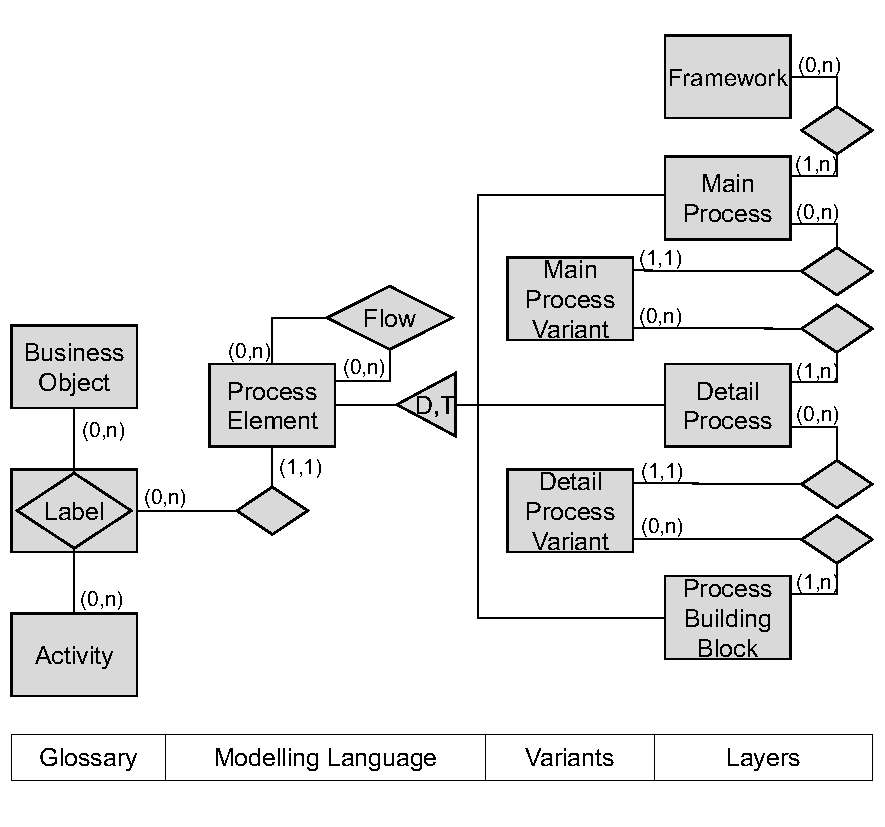
\includegraphics[width=.8\textwidth]{figures/icebricksmetamodel.pdf} \\ \parbox{0.8\textwidth}{\quelle{adapted from \citep[\p{75}]{Puster2015}}}
 	}
	 
	 \end{figure} 
 
	 \subsubsection{Relevance}
	 Relevance refers to the depiction of elements inside the model, which are necessary for the modeling purpose. This causes two boundaries: On the one hand, no element should be included in the model that has no connection to the real world. On the other hand, no aspect of the real world should be part of the model, which does not comply with the modeling purpose. Again, a simple structure of processes helps to guide the modeling procedure. 
	 
	  \subsubsection{Economic efficiency}
	 Syntactical languages are more error prone than semantical languages, because defects occur a posteriori, \ie, after modeling. As a semantical language ensures more guidance and strictness to its modeler, thus less errors exist in the model because they are identified during model creation. This reduces corrections on the outcome, which benefits the economic goal of successfully creating a model for the intended purpose with minimal effort (efficiency). In addition, icebricks as a reference modeling language has the ability to translate into other languages, because it only uses activities and control flow on every level. This enables a more efficient application of the reference model in companies and positively effects learning and use of the language \citep{Muehlen}. 
	 
	 \subsubsection{Clarity}
	 Clarity aims at a clear structure within a model and a simple navigation through different process models. The four layer approach, variant modeling and limited use of branches address a clear and consistent structure in an icebricks process model. Furthermore, the glossary ensures a labeling of processes that conforms to the proposed verb + object construct \citep{7pmg} and tackles the problem of naming conflicts.
	 
	 \subsubsection{Comparability} 
	 With respect to different modeling languages, comparability describes the transfer of content inside a model in language A to another language B without sacrificing information. Icebricks was designed to provide this ability, as the application of a reference model in multiple companies consequently leads to contact with different process modeling languages. 
	 
	 \subsubsection{Systematic Design}
	 The scope of reference models necessitates different layers of detail to manage complexity. Consistence between different layers is a challenge when separate models are built for each layer. By applying a layer structure, variant modeling and the use of a glossary, icebricks guides the modeler during model creation to create well-structured models in the first place. 

	

		\chapter{Case}
%%%%%%%%%%
This chapter serves to connect the scientific background and methodology with the research project. 
It sheds light into the organizational environment, which will be starting point for reference model construction.  

\section{Organizational Setting}
This thesis comes into being as part of the \textit{ERCIS Omni-channel lab powered by Arvato}. This cooperation fosters research in omni-channel CRM through cooperation with Arvato, a leading European outsourcing provider. The focus is set on the CRM services division, which is one of four 
solution groups. While the German market has the largest share, Arvato operates international. The organizational structure can be described as decentralized in the past, but it is intended to integrate the independent country organizations more deeply within the solution group. As clients intensify international outsourcing of customer services to Arvato, a need to deliver an orchestrated outsourcing concept across borders arises. The solution group CRM therefore needs more alignment in their three constituents

\begin{itemize}
	\item Sales \& Business Development,
	\item Portfolio Management \& IT and
	\item Operations.
\end{itemize}

An investigation in organizational structures is not in scope of this work, but this view on the business helps to derive a process structure. As an analogy to the domain of retail, one can see its supply and distribution side in form of Sales \& Business Development and Operations, respectively. The \textit{Sales \& Business Development }organization is oriented towards the outsourcing company, e.g., client. It is the main channel of communication to manage existing and potential clients and hence enables the \textit{supply} of outsourcing contracts and therefore business to the organization.\\
 \textit{Portfolio Management \& IT} organizes available service products and their technological foundation. Especially CRM platforms, their selection and implementation is part of its capabilities. With a decentralized orientation in the past, Arvato faces the problem of a heterogeneous system landscape in client businesses, as there was no guidance for platform selection. The aspired product orientation at Arvato demands standardization in platforms, so that a managed portfolio becomes necessary. As it is a characteristic of CRM outsourcing that clients dictate parts of the environment, \eg, technology or processes, a BPO provider needs to be flexible to react to these requirements. Interface to Sales \& Business Development are the product portfolio, which is marketed to the client. In addition, it supports in design and instantiation of products for a specific client. An internal view of product constituents, namely people, process and platform, is directed towards implementation of services and their operational use. 
  \textit{Operations}, on the distribution side in the retail analogy, is oriented towards the customer. With call center business as core of BPO in CRM, it becomes clear that human resources are one key ingredient of the service delivery.  \\
  
  Drawing from the three described constituents of the Arvato CRM solution group, one can identify three stakeholders in the BPO provider organization. Recalling the BPO Outsourcing chain (\Fig \ref{fig:bpochain}), one part of the provider is linked to the client, another to the customer and the third is located in the center. Applying this logic to the three aforementioned units of Arvato CRM and taking a perspective that is scoped on the essential task of the unit, Sales \& Business Development targets clients and Operations is oriented towards the customers. Distancing from Arvato terminology, one can name these two stakeholders simply \textit{Sales} and \textit{Operations}. \\
  
  Portfolio Management \& IT influences both sides, as well as it acts between the two interfaces. Besides, the central part of the chain can be used to model the stakes of the BPO provider as a whole. With the taken perspective that factors out coordinating activities in the three units, the overall interest in terms of alignment across client businesses and country organizations can be captured in an isolated way. The definition of this stakeholder is necessary, as sales or operations act with focus on their objectives within the organizations and put less emphasis on the provider organization as a whole. This third stakeholder is named \textit{Management}. 
  

\section{Use of a Reference Model for BPO providers in CRM}
\label{sec:refmodusearvato}
The business model of (CRM) outsourcing providers impacts the use of a reference model in the domain. Since the outsourcing service is provided for several clients, the provider’s internal organization has to cope with this kind of diversity. Each client has its own contract and different parts of customer service process outsourced. While in general the business objects to work on (e.g., schedule in workforce management) or process steps (e.g., route incoming call) apply to all clients, they will differ on detail level (e.g., Client A will have a different routing logic as Client B and Client C has routing still in-house and outsources only after this process step).
\todo{checken}
The process differences between distinct client types of CRM outsourcing providers motivate to provide adaptive aspects in the \acrshort{RM} as described in \citep{delfmann2006adaptive}. In a provider model the organization can configure multiple client models based on the provided services that stay compatible and are linked with the provider model. By doing so, the provider model itself gets a reference model characteristics in the organization, while it is an application of the domain model . \Fig \ref{fig:modelleels} visualizes the model levels. The highlighted domain (reference) model is center of this work. The case at Arvato represents a provider model, while businesses of Arvato can be seen as client models. By abstracting from single client business characteristics, the view of a provider is encapsulated in the empirical data that is basis of this work. 
\begin{figure}[caption={Model levels}, label={fig:modellevels}]
	{	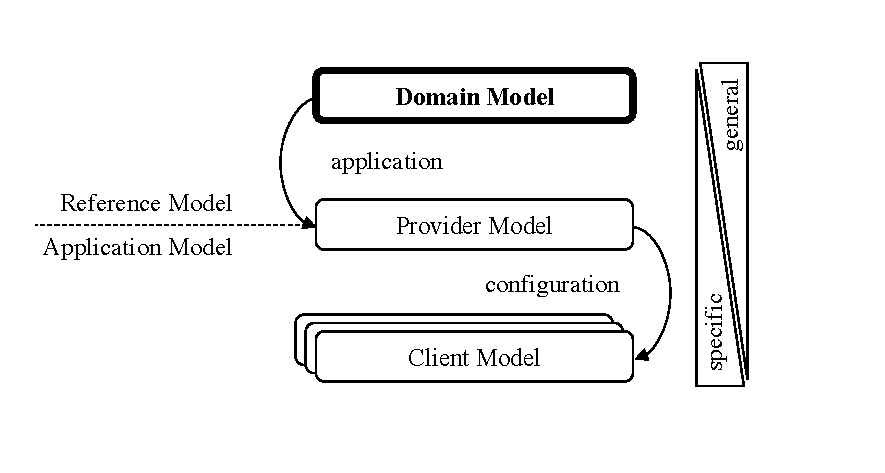
\includegraphics[width=.8\textwidth]{figures/refmodlevels.pdf}}
\end{figure}

The distinction in application and reference model becomes complicated on the provider level. The model is an application of the domain reference model, hence universal validity in the domain vanishes. However, in the domain of the provider this is still valid and has a recommending character as well. With an sufficiently-large client base, diversity of client businesses is captured and therefore the universal applicability is existing to a certain extent. It is noted that sufficiently-large is no further specified here, but Arvato is seen as such a provider\footnote{Arvato is ranked the 6th largest BPO provider 2015 in terms of BPO revenue \citep{hfs2016top}. Explicit numbers for the CRM section of Arvato are not published.}. For this work, the provider model is seen as an application model. Referencing aspects on provider level are considered at construction of the domain level reference model.  

Applying the aforementioned benefits of reference modeling \ref{sec:03_refmod} to the domain in combination with the three stakeholders, one can map these together as in \Tab \ref{tab:refmodbpobenefits}. Therefore it is mandatory to reason the benefits of reference modeling for the different stakeholders in the organization, as design science aims to solve the problem of these parties. The interplay of provider and client model impacts benefits of reference modeling in several aspects and can be attributed mainly to the benefits for Management and Operations.


% Please add the following required packages to your document preamble:
% \usepackage{multirow}
\begin{table}[caption={Benefits of Reference Modelling for BPO-providers in CRM }, label=tab:refmodbpobenefits]
	\centering
	\begin{tabular}{p{1cm} p{2cm} |p{3cm} | p{3cm} | p{3cm} |} 
		\cline{3-5}
		&                                     & \multicolumn{3}{c|}{\textbf{Stakeholder}}                                                                                                                                           \\ \cline{3-5} 
		&                                     & \textbf{Sales}                                          & \textbf{Management}                                 & \textbf{Operations}                                                 \\ \hline
		\multicolumn{1}{|l|}{\multirow{2}{*}{\textbf{Designer}}} & Knowledge                           & \multicolumn{3}{p{3cm}|}{\multirow{2}{*}{\parbox[c]{9cm}{Applicable only to researchers, not to stakeholders in the organization}}}                                                                       \\ \cline{2-2}
		\multicolumn{1}{|l|}{}                                   & Economic benefits from applications & \multicolumn{3}{l|}{}                                                                                                                                                               \\ \hline
		\multicolumn{1}{|l|}{\multirow{5}{*}{\textbf{User}}}     & Cost reduction                      & Faster client approach                                  & Reduced coordination effort                         & More efficient processes                                            \\ \cline{2-5} 
		\multicolumn{1}{|l|}{}                                   & Profit aspects                      & Organized preparation of client meetings                & Standardization facilitates better management       & Usage of new concepts leads to improvement of operational processes \\ \cline{2-5} 
		\multicolumn{1}{|l|}{}                                   & Risk reduction                      & \multicolumn{3}{l|}{\parbox[t]{9cm}{Lower risk of incorrect modeling through reference processes}}                                                                                                  \\ \cline{2-5} 
		\multicolumn{1}{|l|}{}                                   & Analysis                            & Customized offering for approached clients              & Organization-wide benchmarking                     & Benchmarking                                                        \\ \cline{2-5} 
		\multicolumn{1}{|l|}{}                                   & Information Exchange                & Structured communication of value proposition to client & Communication of best practices within organization & Exchange between client operations                                  \\ \hline
	\end{tabular}
\end{table}

BPO is partly cost-driven from a client perspective. For the BPO-provider low costs are therefore a necessity. Cost reduction refers to less effort in coordinating the organization through the used framework and economies of scale and scope across client businesses. For management processes in CRM this means, that a reference process in workforce management enables a more efficient general process on provider level, while on client model level the savings are created. Client-facing processes like sales reduce costs by having a best practice process in the provider model (e.g., run consultative engagements). Operational processes like inbound call handling are always carried out for a specific client and are backbones of the BPO business. While allowing customization in client models, the compatibility to the provider model ensures the connection to reference processes.

Profit aspects often incorporate cost reduction aspects, but stand out through a significant improvement. Realization of up- and cross-selling potentials is one factor, as the necessary steps can be tightly knit into processes. Moreover, historically grown process structures both on client model level and on provider level can be identified. In the CRM domain, improved channel integration through adjusted reference processes benefits both the provider’s abilities towards omni-channel CRM and customer’s perception toward the clients’ customer service, when applied on client model level. As digital channels are becoming the dominant interaction channel, profits through analytics are more in reach.

The analysis aspect expresses the ability to compare and benchmark the business in a new way. Consistent KPI definition enables management to compare across client models, while operations is enabled to improve the analysis of employee performance, as the reference processes cover calculation rules and procedures. As cost efficiency is a primary characteristic in the BPO field, reference modeling supports the provider’s performance management and enables more sophisticated methods through process standardization, especially with respect to more integrated customer service across channels being on the rise.

The last aspect called information exchange phrases the ability \todo{rephrase}to speak a common language in the organization. In the domain of BPO providers this is especially important, because clients vary in their terminology and beliefs of the service. A glossary is seen as an integral part of the reference model to effectively communicate meaning of business vocabulary. As different clients will show different terminology, a consistent management of a general accepted language in the provider’s organization is necessary to ensure comparability. Also, terminology can vary per geographical scope, which adds further complexity and is particularly important for global or multi-national providers. A reference model can propose guidance on this level, while custom definitions in client models will be necessary. Towards client acquisition, the models themselves can be used as basis for discussion, as well as a vehicle to communicate offered services and understanding of CRM.


%

%%%%%%%%%%
\section{DSR Application for Arvato}

 \citeauthor{wilson2002responsible} states that three questions should be asked to research contributions: \enquote{Is it new? Is it true? Is it interesting?} \citep[\p {168}]{wilson2002responsible}. As there is no research found that addresses processes of CRM BPO providers, one can consent the first question. The validity of the artifact, \viz the reference model, is examined on the case at Arvato and aligned with related literature. Regarding the value of this research, one can state the market of BPO amounts approximately 184 billion USD revenue today and CRM services grow above-average \citep{hfs2016top}. As sound processes are critical for both providers and clients. \todo{standardize processes}

\citeauthor{gregor2013positioning} define three levels of design science contribution types, that model the maturity of knowledge in artifacts \citep{gregor2013positioning}. The first level refers to instantiations, \ie situated implementations of an artifact. Level two generalizes by designing constructs, models, that represent knowledge as operational principles or architecture. The highest level positions design theories that hold the most abstract, complete and mature knowledge. 

One research project can build artifacts on multiple levels \citep{gregor2013positioning} and this work aims levels one and two. As the research primarily builds on the case at the research partner Arvato, an instantiation (level one), \viz application in reference modeling terminology, can be undertaken. This serves two purposes. First, it expresses company specifics in comparison to the reference model. Second, it evaluates the use and applicability in a practical use case.  Level two relates to the reference model, that has a higher degree of abstraction. The thesis pursues its construction with priority over the instantiation at Arvato, because there is a unidirectional dependency between the two artifacts: The instantiation has to build on the reference model. The environment in \acrshort{DSR} influences the research and is linked through the relevance cycle. \todo{rephrase}

Following \citeauthor{Hevner2004,Peffers2007}, this work addresses the problem identification and motivation, definition of solution objectives,  design and development. An evaluation is performed based on available information in the exemplary organization and available literature. 


%%%%%%%%%%
%\begin{itemize}%
%	\item wie wende ich DSR hier an?%
%	\item warum wende ich DSR hier an?
%	\item was decke ich mich dieser arbeit ab?
%\end{itemize}

%%%%%%%%%%
\subsection{Problem Identification}
%Activity 1. Problem identification and motivation. Define the specific research problem and justify the value of a solution. Since the problem definition will be used to develop an artifact that can effectively provide a solution, it may be useful to atomize the problem conceptually so that the solution can capture its complexity. Justifying the value of a solution accomplishes two things: it motivates the researcher and the audience of the research to pursue the solution and to accept the results and it helps to understand the reasoning associated with the researcher’s understanding of the problem. Resources required for this activity include knowledge of the state of the problem and the importance of its solution.
CRM is characterized by the components people, process and technology \citep{Chen_2003}, hence BPO outsourcing in this domain needs to address these three components. Here, processes stand in focus.  \cite{schewe2007} see BPO as synthesis of outsourcing and process optimization. The latter necessitates coordination between provider and client, which would benefit from a common basis to build up on. In case of CRM, the distinctiveness of customer contact through the provider adds a challenge that is not typical for BPO in general. 

Diversity in outsourcing contracts require an abstract view on processes, so that the organization can benefit from an appropriate model that enables use of synergies. In case of Arvato CRM, one challenge stems from a decentralized organization, that adds an additional organizational layer which conflicts with company-wide alignment. International clients also demand solutions across countries, which are hard to accomplish without a common understanding. The challenge is rooted in the decentralized internal structure and intensified by complexity of the outsourcing field (\eg, \acrshort{CRM}).

The change to a digital society and with it the increase in contact channels, thereby requiring multi- and omni-channel management, makes an isolated view of channels impractical. \acrshort{IS} need to be designed in order to handle, integrate and make use of diverse channel data for a better customer experience. As BPO providers cannot rely on single systems (\cf \ref{sec:bpocrmis}) which may provide a documented process tailored to the system, a more general representation is needed. Bringing together these aspects formulates a crucial problem for providers and identifies a research gap. 


%wert meiner lösung:
%strukturierung der bpo prozesse.aus unternehmenssicht. grundstein in bpo in crm, aber grundstein für %bpo referenzmodell  
%einführung der levels zur strukturierung der provider / client sichten. erster schritt zu einem bpo %referenzmodell. 
%berücksichtigung von omnichannel crm. 

%%%%%%%%%%
\subsection{Solution Objectives}
%anforderungsdefinitionen nach püster
%der kasten: thomas 248, vombrocke 98, püster 63, 

%%%%%%%%%%
%Activity 2. Define the objectives for a solution. Infer the objectives of a solution from the problem definition and knowledge of what is possible and feasible. The objectives can be quantitative, e.g., terms in which a desirable solution would be better than current ones, or qualitative, e.g., a description of how a new artifact is expected to support solutions to problems not hitherto addressed. The objectives should be inferred rationally from the problem specification. Resources required for this include knowledge of the state of problems and current solutions, if any, and their efficacy.

Based on identified problems, solution objectives outline requirements, that the reference model artifact should contain. A morphological box helps to structure reference model attributes. This pattern draws from the work of \cite{Puster2015} and \textbf{highlights} pursued characteristics in \Tab \ref{tab:morph}.  

\begin{table}[caption={Reference model requirements }, label=tab:morph]
	\centering
		\begin{tabular}{ 
				p{3.1cm}  
			p{2cm} p{2cm} p{2cm} p{2cm} p{2cm} p{2cm} p{2cm} p{2cm} p{2cm} p{2cm} p{2cm} p{2cm}    }
			Attribute                                   & \multicolumn{12}{c}{ Characteristic }                                                                                                                  \\ \hline
			\multicolumn{1}{|l|}{\textit{Reusability}}          & \multicolumn{6}{c|}{\textbf{generic reference model}}                       & \multicolumn{6}{c|}{non-generic reference model}                  \\ \hline
			\multicolumn{1}{|l|}{\textit{Purpose}}              & \multicolumn{6}{c|}{\textbf{organizational design}}                         & \multicolumn{6}{c|}{application system design}                    \\ \hline
			\multicolumn{1}{|l|}{\textit{Description level}}    & \multicolumn{4}{c|}{\textbf{concept}}                & \multicolumn{4}{c|}{data processing concept} & \multicolumn{4}{c|}{implementation}       \\ \hline
			\multicolumn{1}{|l|}{\textit{Description type}}     & \multicolumn{4}{c|}{\textbf{As-Is}}                  & \multicolumn{4}{c|}{To-Be}                   & \multicolumn{4}{c|}{Ideal}                \\ \hline
			\multicolumn{1}{|l|}{\textit{View}}                 & \multicolumn{3}{c|}{organization} & \multicolumn{3}{c|}{data}    & \multicolumn{3}{c|}{functions}   & \multicolumn{3}{c|}{\textbf{process}} \\ \hline
			\multicolumn{1}{|l|}{\textit{Knowledge generation}} & \multicolumn{6}{c|}{\textbf{induction}}                                     & \multicolumn{6}{c|}{\textbf{deduction}}                                    \\ \hline 
			\multicolumn{13}{r}{Adapted from: \citep[\p{63}]{Puster2015},\citep[\p{98}]{brocke2003referenzmodellierung}, \citep[\p{248}]{thomas2006mang}  }       
			
	\end{tabular}
\end{table}

In terms of reuseability, the reference model is intended to be generic, so that it is reusable for a class of companies. Here, these are providers of business process outsourcing in customer relationship management. With the previously discussed provider models, one can name a non-generic reference model. Distinguishing processes of the domain are prioritized in the construction, as their value contribution to the model is higher in comparison to generic processes, that do not differ significantly from other domains (accounting for instance).  

The purpose of the model is seen in organizational design. Drawing on the listing of use cases given by \cite{Rosemann2012proc}, knowledge management and organizational documentation can be named in the first place. 

The \acrshort{ARIS} introduces three different conceptual levels with increasing IT-orientation. The reference model is seen on concept level, which facilitates comfortable communication with the business. 
\todo{+++}

Regarding the description type, one can separate into three three model orientations. As-is aims to describe the current state of the domain, \viz showing common practices. To-be models a future state that incorporates wanted changes. \todo{ideal?} Ideal modeling displays an optimal scenario. In this case, the intention is to capture the current state of the domain. 

The process view integrates the organizational, data and functional perspective. It is noted that the time-logical sequence of processes may be of subordinate importance, as an application probably causes reordering of process steps. Nevertheless, the process view is the medium for capturing aspects from other perspectives, while leaving room for individual adjustments without sacrificing model integrity. 

As mentioned before, induction and deduction are employed for knowledge generation.
 
\subsubsection{General objectives}
Combining these attributes implies demands, that relate to the solution objectives.

\hfill\begin{minipage}{\dimexpr\textwidth-1.2cm}
	\textbf{Solution Objective 1}: Construction of a generic  reference model that covers distinguishing processes for BPO-providers in CRM on concept level
	\\
	
	\textbf{Solution Objective 2}: The reference model can be applied for use at Arvato CRM.  
	\\
	
	\textbf{Solution Objective 3}: The construction  process is well-documented, makes use of empirical research by induction, which is enriched by deduction from \acrshort{BPO} and \acrshort{CRM} theory.
	
	\xdef\tpd{\the\prevdepth}
\end{minipage}

The choice of the modeling language should not interfere with the intended use in the industry. As no studies regarding process modeling language use are available to the best knowledge of the author, the language should be transferable into popular candidates, \eg \acrshort{BPMN} and \acrshort{EPC}. For reference modeling as such, there is neither a standard existing, but a trend towards use of existing languages exists \citep{Fettke2004}. 

While reference models aim for content-wise standardization, the use of formalized languages helps to sustain syntactic and semantic quality in the model \citep{Fettke2004}. By doing this, the model should be comprehensible with ease from members of the business and IT organization. 

\hfill\begin{minipage}{\dimexpr\textwidth-1.2cm}
	\textbf{Solution Objective 4}: A syntactic and semantic formalized process modeling language is used, that is transferable to other languages. 
	
\end{minipage}

\subsubsection{Stakeholder-related objectives}

Building on the discussion in \ref{sec:refmodusearvato}, the benefits of reference modeling in the domain are stated. Putting objectives of this work in direct relation to the three identified stakeholders is difficult, as the model represents the whole provider organization. The overall goal of increased alignment reasoned the decision to create this model at the research partner on a board level. However, the stakeholder's benefits do not directly create objectives. The construction merely should consider realization of the identified benefits, by incorporating requirements for their realization.  Consequently, these requirements are formulated as objectives.  

The organization uses an application model (provider model) that draws from the reference model, which is discussed in this work. Hence, stakeholder-related objectives are motivated by an application model and then mirrored towards the reference model. In this regard, the following paragraph uses the term model to express this ambiguity. 

Sales is oriented towards clients and the model is a means to communicate more effectively with them. Their interest externally lies in a use as a statement of competence. The management uses it to encompass idiosyncrasies across client businesses. Thereby it facilitates alignment, which is incorporated in the use of reference models for organizational design (\cf \Tab \ref{tab:morph}). Operations is supported by the model to handle complexity of increasing channels and benefits from reference processes, as they enable standardized approaches. \todo{+++}
\\

\hfill\begin{minipage}{\dimexpr\textwidth-1.2cm}
	\textbf{Solution Objective 5}: The model can be used as a statement of competence for sales activities towards clients.
	\\
	
	\textbf{Solution Objective 6}: The model holds a process representation, which supports a common understanding across client businesses. 
	\\
	
	\textbf{Solution Objective 7}: The model is able to represent an omni-channel environment. 

\end{minipage}


\section{Limitiations}
%%%%%%%%%%

The title of this thesis expresses limitations in two ways. Firstly, its research is \textit{towards} a reference model. It is not intended to complete the model with this work. It lays a foundation for detailed investigation in its components. Processes are only partly described on the lowest detail level. Also the focus is set on distinguishing processes in the domain, which neglects support processes as defined in \ref{processorientation}. The simplification in this thesis can be justified by the fact that the contribution to the knowledge base is insignificant for support processes, as these are subject to publications beyond number. 

Secondly, \textit{a reference model} is meant, which signifies limitations in used data to construct the model. As the primary data source the research partner and its organization as an example of a BPO provider in CRM, one can object the dispensation of an investigation in other providers. However, due to the nature of the BPO business with multiple client businesses and the size of the research partner, diversity is captured to a certain extent. 

While the process view includes aspects of the data, organizational and functional perspective, especially a dedicated data view would be beneficial to out research in an omni-channel environment. The integration of data to identify customers across channels is an important, yet unsatisfactory explored research area. In this regard the process reference model helps to convey a perspective of activities from a time-logical order, to identify and structure moments that are important \wrt data availability, access or creation. 

Regarding the structure of domain, provider and client model, it is noted that this proposal is only outlined in this work and not further described through generic reference modeling techniques, as discussed in \cite{delfmann2006adaptive, brocke2003referenzmodellierung}. 

The thesis puts special emphasis of customer service processes (\cf \ref{sec:crm},  \Fig \ref{fig:crmprocessfr}). Outsourcing operational \acrshort{CRM} may also be leaned towards other operational processes of CRM, like marketing or sales. However, customer service is the most frequent case, while clear boundaries vanish. This reasons the framing of the reference model in \acrshort{CRM} instead of customer service. 

%\begin{itemize}
%	\item only core processes specified, as also done in retail-h ok
	%\item core processes partly on lowest level
%	\item process refmod, not data,...
%	\item provider, client model construct only outlined 
%	\item specified later
	%	\item one company
%\end{itemize}
%%%%%%%%%%


		
\chapter{Reference Model Construction}
%%%%%%%%%%

This chapter conceptions the process reference model and is central part of this thesis. In order to discuss particular processes, the framework itself needs to be discussed. What follows is the discussion of processes, which puts special emphasis on design decisions, \viz \textit{how} to model certain aspects by means of the language icebricks. 

	%%%%%%%%%%
	deloitte W14: managing change dispute:::: innovation und so... wichtig für begründung des frameworks
	\section{Process Framework}
	
	\citeauthor{Meise2001} defines a framework as \enquote{an ordering of relevant elements and relationships on a high level of abstraction. [...] Purpose is to give an overview about an original and to support structuring of elements and relationships on lower detail levels} \citep[\p{62}]{Meise2001}. Drawing further on his work, which especially targets framework design in process-oriented organizations, the proposed procedure for construction is adopted (\Fig \ref{fig:meise}). Differences to his approach arise, as the reference model displays an as-is state of the domain and does not follow goals of reorganization set by a specific company. Therefore, the \textit{organization} represents a fictive BPO provider in CRM in the following, which captures generic aspects of the domain. The construction is split into two components. The structural part first encompasses strategic and fundamental reflections, while the graphical component transfers these into a visual form that supports communication.

	\begin{figure}[caption={Procedure for framework construction}, label={fig:meise}]
		{	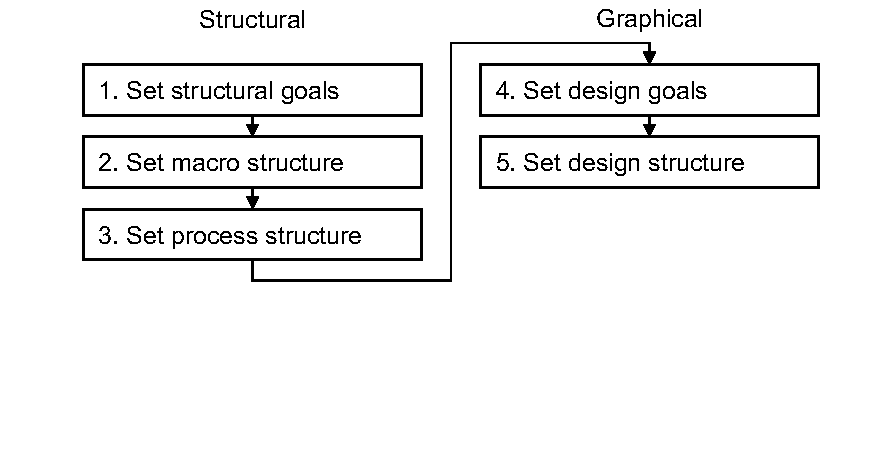
\includegraphics[width=.8\textwidth]{figures/framework-meise.pdf}}
		\hspace{6.2cm}	SOURCE:  adapted from \citep[\p{122}]{Meise2001}
	\end{figure} 
	
	\subsection{Set structural goals}
	
	Modeling is no end in itself and different purposes require different models. Theoretically speaking, purpose of this research is to create an artifact that generates utility and tackles a problem in the real-world.  Previously identified problems (\ref{sec:proide}) lead to objectives (\ref{sec:solobj}) which are to be faced with the process reference model in general and its framework in particular. The existence of general (organizational) and stakeholder-related objectives requires the framework to bring together both ends.
	
	\begin{table}[caption={Solution Objectives}, label={tab:solobj}]
		\centering
		\begin{tabular}{l p{13.3cm}}

			\textbf{No. }&\textbf{ Solution Objective}
			 \\ \hline
			\textbf{1 }                        & Construction of a generic reference model that covers distinguishing processes for BPO-providers in CRM on concept level.                                                    \\ \hline
			\textbf{2}                         & The reference model can be applied for use at Arvato CRM.                                                                                                                    \\ \hline
			\textbf{3 }                        & The construction,process is well-documented, makes use of empirical research by induction, which is enriched by deduction from \acrshort{BPO} and \acrshort{CRM} theory. \\ \hline
			\textbf{4}                         & A syntactic and semantic formalized process modeling language is used, that is transferable to other languages.                                                              \\ \hline
			\textbf{5}                         & The model can be used as a statement of competence for sales activities towards clients.                                                                                     \\ \hline
			\textbf{6}                         & The model holds a process representation, which supports a common understanding across client businesses.                                                                    \\ \hline
			\textbf{7}                         & The model is able to represent an omni-channel environment.                                                                                                                 
		\end{tabular}
	\end{table}

	
	
	\subsection{Set macro structure}
	
	A framework, as a strategic tool, incorporates concepts of strategy. One can name two perspectives, namely a market- or resource-based view of strategy, which are directed externally or internally, respectively. They are not independently of each other, but their interplay is seen as an important factor in strategic decision making. Literature criticizes that standardization through reference model application has contra-productive effects on strategic competitive advantages. \cite{becker2004handelsinformationssysteme} note that the argument is true, when the reference model is used as an application model. However, the application of the reference should incorporate strategic characteristics of the company. This reference model framework is designed in a way that generic strategic orientation for providers is incorporated. 
	
	The market-based view follow the structure-conduct-performance paradigm, that explains success of a company through external factors in the industry. \cite{porter1980} formulated the so called five-forces model, which describes bargaining power of suppliers (1), threat of substitutes (2), bargaining power of buyers (3), threats of new entrants (4) and industry rivalry (5) as determinants of competition. Applying these two the BPO domain, a trivial substitute for outsourced services is the return of services inside the parent organization. Further, the substitution of customer services through automation may render outsourcing obsolete. The bargaining power of suppliers and buyers can be loosely mapped to clients and customers. While clients as suppliers clearly influence the provider directly, customers show less of this influence on the outsourcing provider. As the provider takes an intermediate position between client and customer (\cf \Fig \ref{fig:bpochain}), their acting is always in connection with the client. However, an assessment of outsourced service quality puts pressure originating from the customer on the provider, which in turn will also be judged by the client. The entry of new players on the market (4) can be tackled by barriers, that go back to competitive advantages of differentiation or cost-leadership. While the latter is especially causing fierce competition in low-wage regions that realize offshore-outsourcing, outsourcing players in CRM that feature more profound services, lean towards a differentiation strategy. This can also be stated for Arvato. Lastly, industry rivalry among players in the BPO CRM market is also influenced by the aforementioned generic strategies, to position established companies. A framework adopts market-based aspects through accounting for markets or segments therein. These are accompanied by business units or processes that relate to this external environment. 
	
	The resource-based view of strategy \citep{wernerfelt1984resource} analyzes internal strengths and weaknesses. Resources are bundled to form capabilities and should be rare, inimitable, create value and be non-substitutable. Due to asymmetries of resources, competitive advantages are enabled. The identification of capabilities of CRM BPO providers (\cf \ref{sec:bpocrmis}: operational and business development capabilities) can only be done on a generic level for the reference model. Application necessitates specifying the framework to conform to company-specific capabilities. The operational capability should reflect the operational process component in CRM (\cf \ref{fig:crmprocessfr}), and service delivery from the outsourcing side (\cf \ref{app:provproc}). Business development, \ie understanding and addressing client needs, misses a pendant in an isolated CRM view, but can be put in relation to delivery management in the outsourcing model. 
	
	Putting both views together emphasizes the client and customer market environment and two capabilities, that relate to these markets. Towards the client side, providers are criticized by clients for being too reactive instead of proactive (49\%), delivering poor service quality (48\%) and lack of innovation (37\%) \citep{deloitte2014outsourcing}. While the first point of criticism addresses the client relationship, the other two are directed towards the service itself. Looking at the constituents of \acrshort{CRM}, the people, process, technology split draws a line to the resource-based view, as these three resources need to be developed and captured to enable superior service provision for clients. Apart from the  \acrshort{CRM} view, these three also have their own meaning in \acrshort{BPO}. \todo{Gross} The importance of processes in  \acrshort{BPO} is obvious. The people component can be interpreted here as the provision of manpower and their training for services; (information) technology as an enabler of outsourcing (\cf \ref{sec:bpo}) . 
	
		
	\subsection{Set process structure}
	\label{sec:procstr}
	Given that the model shows processes, the structural split of people, processes and technology is hardly meaningful, as two aspects of  \acrshort{CRM} or \acrshort{BPO} would be left out. Drawing from the BPO chain and the identified stakeholders enables another categorization that leaves room for design choices, while capturing generic aspects of business processes within \acrshort{BPO}. As \acrshort{BPO} is the framing construct and  \acrshort{CRM} one use of it, this order is to be prioritized. The following briefly describes business processes, that are detailed in the remainder of this chapter.
	
	
	\begin{figure}[caption={BPO chain provider scope with stakeholders}, label={fig:bpochainscope}]
		{	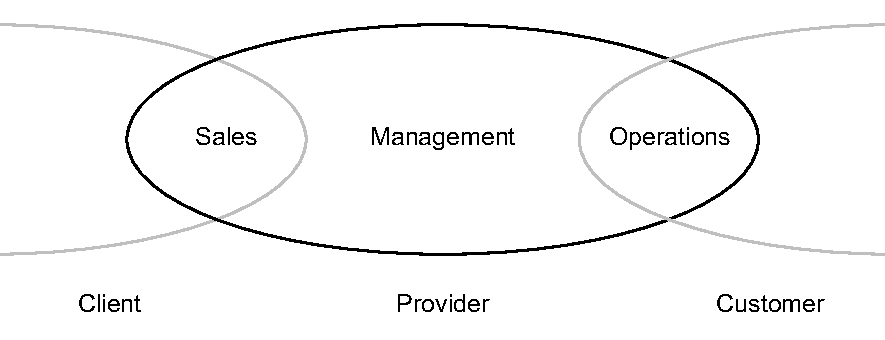
\includegraphics[width=.8\textwidth]{figures/chain2.pdf}}
	\end{figure} 
	
	\subsubsection{Sales-related}
	Sales-related business processes cover processes that have touchpoints with the client. These take place along a lifecycle, which starts with initial contact between provider and client, and hopefully advances through creation of an outsourcing contract. For this agreement, the \acrshort{BPO} provider places its products (\ie, service blueprints) in the clients requirements profile to create solutions for identified problems. Also, the transition and setup of the outsourced business must take place. After everything is set up, the client relationship is maintained under the umbrella of account management. 
	
	\subsubsection{Management-related}
	The management-related business processes bring together resources in the provider organization, so that the operations and business development capability are realized. Regarding the latter, it is important to have a products in place, which can be implemented as service solutions for clients.  \citep{schewe2007} names this delivery management, but explicitly refers to its similarities with product development. In addition to the development, the management of existing products inside a product portfolio becomes important. 
	
	Benefits through economies of scope are a question of offered services and not processes. The operations capability can be addressed by processes, that enable economies of scale. These are realized by the increased output of services across client businesses, which in turn necessitates alignment in these services so that their output can be counted \textit{together}. This alignment is facilitated through a product-view of services and their underlying portfolio in the organization. In addition, people in the provider organization need to be trained  in order to excel in the role of \acrshort{CSR}. Their career path can be seen from a process perspective, so that a strong relationship is established with their employer. This aspect shall be called People Lifecycle Management\footnote{The term people is preferred over agent or \acrshort{CSR}, because it puts this process strongly in connection \acrshort{CRM}. As the management-related processes are tried to be references for \acrshort{BPO} in general, this is not intended.}.  Lastly, management of the workforce, especially scheduling, becomes critical in a business like customer service. The assurance of the right capacity at the right time to meet fluctuating demand with little waiting time is expected from the client. Therefore, efficient techniques to manage the complexity of multiple channels, different demand patterns and different skilled \acrshort{CSR}s are necessary. This is encapsulated in the process of workforce management. 
	
	\subsubsection{Operations-related}
	The last group of business processes target the service delivery in the words of \citeauthor{schewe2007}. The processing of transactions with customers is in focus, which can be on numerous channels. A transaction in this case is a conversation, so that theories of communication \citep{shannon1949} may be used here.  A message is sent from a sender to a receiver through a medium. In case of customer service, both the customer or the \acrshort{CSR} can start a conversation, that has a subject which relates to the client in some way. Reasons for contact may be separated by being related to a previous transaction. This transaction might be a purchase of a client's good or service. The communication channel increasingly varies and is no reasonable split \todo{was für 1 split}, as in an omni-channel environment a seamless experience across channels is intended. Hence, the processes should be similar on a high level of abstraction. 
	
	Communication can be asynchronous (\eg, e-mail) or synchronous (\eg, voice), which puts emphasis on temporal differences in the conversation. While the employed process definition encompasses the \enquote{time-logical sequence of activities}, the value (\viz time between activities) does not impact the process logic itself, as this is a question of succession. General steps in inquiry handling from a business perspective will be similar independent of the (a)synchronous case. What becomes more important from a business perspective is the question after the contact initiator. A communication triggered by the customer (incoming) follows demand patterns that are inferred from historic data, while better planning of \acrshort{CSR} opened contacts (outgoing) is possible, as the temporal decision of contact lies at the business and not the customer. 
	
	Lastly, one has to differentiate in customer contact whether \acrshort{CSR}s are involved in inquiry handling, which obviously has business implications. When customers use self-service to address their needs, software takes the \acrshort{CSR} role, which saves resources. Providers can differentiate themselves through expertise in these systems. Clients save money by less volume that is processed by humans (employees of the outsourcing provider). At first sight, this may cannibalize outsourcing business, but the expertise of installing and running these self-service systems is likely not located in clients that outsource \acrshort{CRM}. Consequently, providers can generate new business by accumulating know-how in self-service activities. On the one hand, they design the customer-facing self-service in order to handle the inquiry (which by definition are customer-initiated). On the other hand, the provider manages and maintains the knowledge base, that sits behind these automatons in the back-end. This knowledge management does not only have implications on self-service, but also on other customer contacts, as the \acrshort{CSR}s in the human-to-human communication also query the knowledge base to solve customer problems.  
	
	It is desisted from the explicit modeling of a customer journey, because it encompasses components that cannot be part of a process model for providers. The model in this thesis is centered on the outsourcing provider. Modeling of a customer journey requires a customer-centric model, which then contains steps of the customer journey in a detailed way. Such a model should be a \textit{playground} for identifying space for improvement in dialog with a client regarding its customer journey. In addition, it would benefit from avoiding the standards of process models, as its purpose is seen in the \textit{design} of a journey through \acrshort{CRM} components. Research from the field of marketing can be a starting point \citep{Lemon_2016, Frow_2007}. 
	
	\subsection{Set design goals}
	
	The visual representation of the framework is linked to its cognition among viewers, therefore it needs to support the communication of the reference model's purpose. In contrast to language-processing, the process of perception is foregrounded, as the graphic is processed all at once and not sequentially. The model has to capture the fundamental characteristics of the domain of outsourcing at first glance. The sketched model level when applied (provider and client model) should be visually supported, as the framework of the reference is the blueprint to convey this hierarchy. 
	
	\hfill\begin{minipage}{\dimexpr\textwidth-1.2cm}
		\textbf{Design Goal 1}: The framework has to visualize the business of BPO providers.
	\end{minipage}

From a process perspective, as well as to reduce complexity, it helps to highlight important business processes over supporting or coordinating processes. By doing this, the viewer gets an impression about central parts of the model. 

	\hfill\begin{minipage}{\dimexpr\textwidth-1.2cm}
	\textbf{Design Goal 2}: The framework has to distinguish business processes from other process types. 
\end{minipage}

Furthermore, provisioned services are to be shown. In order to gain an understanding of characteristics in CRM outsourcing, especially in an omni-channel context, the framework has to clearly communicate their orientation towards the customer. As it is the differentiating aspect towards BPO for other processes, this fact could be incorporated in the design.  

	\hfill\begin{minipage}{\dimexpr\textwidth-1.2cm}
	\textbf{Design Goal 3}: The framework has to cover the CRM-orientation in service provision. 
\end{minipage}

A framework's purpose is to manage complexity by displaying relevant elements. In addition, the visual representation should be clear, consistent and structured to enable understanding on its own. 

	\hfill\begin{minipage}{\dimexpr\textwidth-1.2cm}
	\textbf{Design Goal 4}: The framework has to be easily processable by viewers without further explanation. 
\end{minipage}

	\subsection{Set design structure}
	
	The design of the reference model primarily addresses reference model users. However, its design will have large influence on the depiction of an application model. It is noted that the framework is designed independent of a process modeling language. The use of a reference design (model) can serve as a basis, as it includes benefits that have been previously discussed in context of reference models. The house reference design for example is used in the Retail-H (\ref{mod:retail}).
	
	Known patterns influence human perception \citep{kroeber1997} and can transfer associations. In case of the house reference design, one can link solidity, stability and security \citep[\p{216}]{Meise2001} with it. It is made up on three parts (\viz roof, core, foundation), which can be used to visualize coordination, main and supporting processes, respectively. The foundation represents a basis on which the house is built. Its main part, biggest in size, stands in the center and has the largest impact on the perception of the house's content\todo{ref becker}. The roof brings together underlying elements and has an analogy towards an organizational hierarchy. 
	
	\subsubsection{Framework composition}
	
	Adding the previously discussed process structure, supported by the BPO-chain design, one can convey this representation into the core area. \Fig \ref{fig:frameworkdesign} shows influences for the framework components. 
	\citeauthor{Meise2001} proposes the use of a value chain representation with a chevron that enables linking of multiple elements, which is called a \acrfull{VACD}. It communicates the input, transformation, output relation of a company, as the area on the left or right hand side of the house can be used to model supply or distribution markets. 
	These two markets are existing in BPO with end-customer interaction (like in \acrshort{CRM}), which nicely brings together house reference design and \acrshort{BPO}-chain. 
	
	\begin{figure}[caption={Framework design influences}, label={fig:frameworkdesign}]
		{	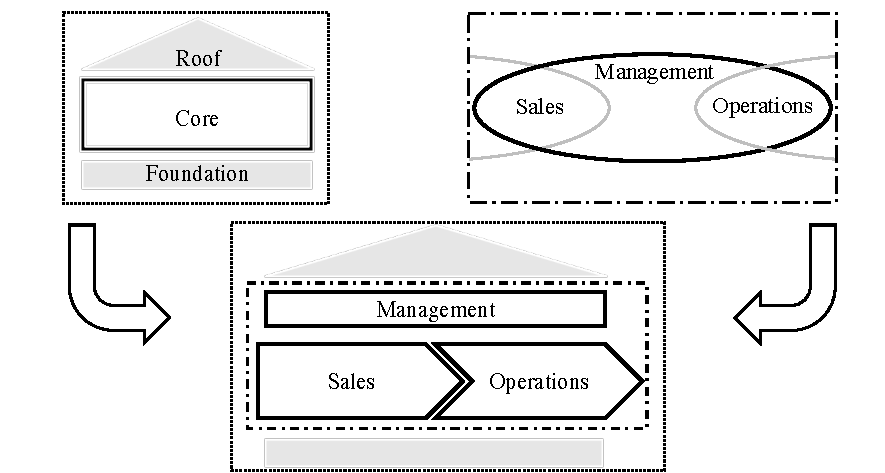
\includegraphics[width=.8\textwidth]{figures/frameworkdesign.pdf}}
	\end{figure} 
	
	
	The value chain can be represented by the exclusive use of chevrons that are linked together or it can have one starting element, which is a pentagon. This element is \textit{closed} to the left side in contrast to the \textit{open} chevrons. Porter uses the \textit{closed} variant, where the widened interface to the left side is emphasized. As the left side of the framework represents the client side, the strong link to the outsourcing partner shall be highlighted \wrt the customer-facing right hand side. Here, the interface to the customer shall be pointed for the following reasons. First, the interaction with a customer is intended to be independent of communication channel, so that the idea of omni-channel is conveyed (and with it the \textit{one face to the customer}-paradigm). Second, the customer-centric idea is communicated with this representation, as all actions towards him (the complete height of the chain) is pinpointed towards one customer. The process structure of three elements consequently locates sales processes on the left and starting part of the value chain and connects the operations processes with it, so that the client and customer side is represented. The value chain is deliberately wider than the house to make its function as an interface to the adjacent markets clear. The 
	
	The management processes are located above the value chain and spans the complete width of the house. While it is part of the core, it does not have a \acrshort{VACD} representation, as it has little contact with the the client or customer. However, it influences the complete part of business and is a indispensable part of the \acrshort{BPO} provider business, hence it must be part of the core instead of the roof. Sales processes benefit from the product and portfolio management, while workforce- and agent-related processes are scoped towards service delivery and with it operations. Reason for locating it at the top of the \acrshort{VACD} is that these processes include tactical to strategical aspects, that influence the underlying processes in the framework's core. 
	
	\subsubsection{Framework details}
	
	Locating the identified processes on the framework needs to be done carefully, as their position and shape is important for the viewer's perception. The three areas of the framework's core narrow down positioning alternatives. Their size and shape is equal, to emphasize their main process feature. Customer facing processes vary slightly. Support and Coordination processes have a smaller boxes, font size and slimmer boarders to limit their attention. \Fig \ref{fig:framework} shows the framework.
	
		\begin{figure}[caption={Framework}, label={fig:framework}]
		{	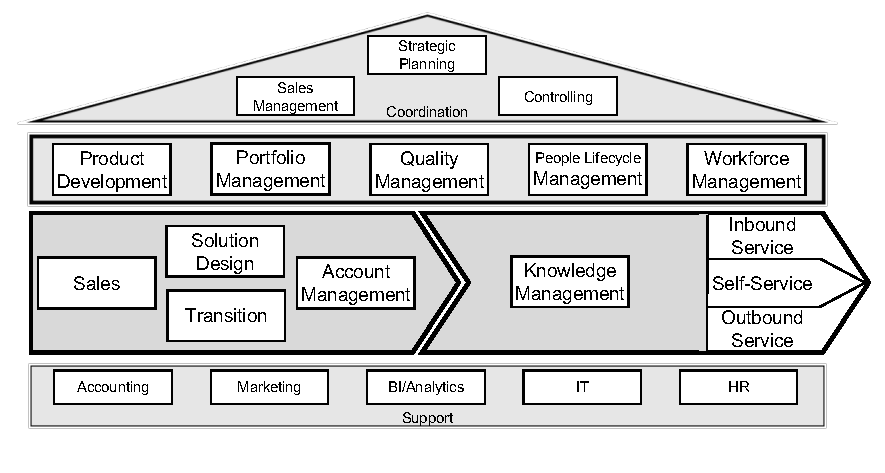
\includegraphics[width=.9\textwidth]{figures/framework.pdf}}
	\end{figure} 
	
	
	 Starting with sales-related processes, the main processes Sales, Solution Design, Implementation and Account Management have to be placed on the framework. As explained in \ref{sec:procstr}, they follow a life cycle, so that \textit{Sales} leads to \textit{Solution Design} and \textit{Implementation}, while existing clients relationships are cared in account management. This leads to a positioning of Sales as the leftmost and \textit{Account Management} as the rightmost process within the sales area. Implementation and Solution Design are processes that take between the previous ones. They are both part of the setup of a business and are hence located next to each other. 
	 
	 Operations processes have the peaked customer interface as starting point for locating processes. These are split into \textit{inbound}, \textit{outbound} and \textit{self-service} as customer facing processes, that are accompanied by\textit{ knowledge management} as an process that takes place without knowledge of the customer. Consequently, knowledge management is located towards the center of the framework and less directed to the customer. The other three processes share their direct customer contact and are therefore in the right part of the chevron. To emphasize their role as the interface to the customer, their representation is adjusted to link to the customer. Furthermore, they are also located on the same height in the flow of the chain to highlight that these are alternatives of contact. By making no distinction of channels on framework level, their equality of treatment is represented. Inbound is written on top, as it is the most important process by volume in among the three, when one sets focus on customer service.
	 
	 The four management processes are located next to each other in their area on top of the \acrshort{VACD}. The product and portfolio processes have higher connection to the client side, as these service products are sold to  clients. The \textit{product development} process has a stronger external relation, as new products should meet unsatisfied demands from the market. \textit{Portfolio management} on the other hand is an intra-organizational process that sets its focus on the provider. The other two processes, namely \textit{People Lifecycle Management} and \textit{Workforce Management} impact \acrshort{CSR}s. Their positioning can be reasoned through an higher impact of workforce management on the service delivering activities through schedules, plans and forecasts of customer demand. People Lifecycle Management on the other hand is again oriented towards the provider organization, because the management of human resources for service delivery is of direct interest for the provider, but not to the customer.
	 
	 Support and coordination processes are not further specified in this thesis. Their elements are inspired by general processes of companies that play a role in \acrshort{BPO}. Processes like accounting or marketing are obvious to fulfill financial regulations and position the provider on the market, respectively. \acrfull{BI} / Analytics captures the process of supporting the business through data-driven insights apart from implemented solutions, as well as to provide decision-support for management on a tactical or strategic level. The latter emphasizes especially the  \acrshort{BI} aspect and would also make a positioning in the roof considerable. However, analytics was added to this process as no clear border between the two can be defined in the literature  \citep{mertens}. \citep{Chen:2012:BIA} suggest the term \acrshort{BI} \& Analytics. Interpretation of the two notions will vary in an application, as it depends on the understanding in the target organization. IT supports the business through operation of systems (for instance in accounting, HR or for decision-support in management). HR manages people in the provider organization and is different from People Lifecycle Management, as it focuses on \acrshort{CSR}s, not personnel management in general. Sales Management as a coordination process is subject to planning of client businesses and verticals. It is located on the left side of the roof to move it closer to the sales processes. Strategic Planning guides the provider organization as a whole with a long-term perspective. It is located highest in the roof to emphasize its importance for the strategic management of the organization. Controlling completes the coordinating processes by supplying the management with information and overseeing the client businesses. 
	 	 
	 \subsubsection{Addressing  the design goals}
	 
	 	 	\begin{table}[caption={Design Goals}, label={tab:desobj}]
	 	\centering
	 	\begin{tabular}{l p{13.3cm}}
	 		
	 		\textbf{No. }&\textbf{ Design Goal}
	 		\\ \hline
	 		\textbf{1 }                        & The framework has to visualize the business of BPO providers.                                     \\ \hline
	 		\textbf{2}                         & The framework has distinguish business processes from other process types.                                                                                                                   \\ \hline
	 		\textbf{3 }                        & The framework has to cover the CRM-orientation in service provision. \\ \hline
	 		\textbf{4}                         & The framework has to be easily processable by viewers without further explanation.                                                              
	 		
	 	\end{tabular}
	 \end{table}
 
	 
	 With the proposed framework shown in \Fig \ref{fig:framework}, the four design goals are achieved. Its fundamental structure with the \acrshort{VACD} shows encapsulates the BPO business and by exchange of the right chevron, one can apply the model to other domains than \acrshort{CRM}. The relevance of business processes is highlighted through use of the house reference design. The right chevron is suited to represent service delivery in  \acrshort{CRM} through focus on customer contact, while abstracting from explicit processes for offered services (products). These are contained in the product development, solution design and portfolio management process without specifying of measures. Naming these would conflict with the intent of a reference model, as these will be different for companies in the domain. A minimalistic two dimensional representation without additional distracting features such as color or varying fonts supports understanding of the framework. The different shapes are limited and the use of rectangles is preferred. Other elements, like the \acrshort{VACD}, are associated by the viewer and naturally convey the flow of the framework: the outsourcing client's \acrshort{CRM} is given to the provider, who then adds the value to the chain and sends it to the customer. It is noted that application of the reference model results in differences in content, but also in design (to conform to corporate design for instance). However, an empirical evaluation of this framework design was not conducted so statements about viewer's opinions are derived from design choices of the author. \todo{rephrase}
	 
	 The following dives into the process models below the framework. The icebricks language is used to meet solution objective 4 and hence the underlying structure below the main processes on the framework is composed of detail processes, which in turn have process building block underneath. 
	 
	 
	 %%%%%%%%%%
	 \section{Customer Processes}
	 \todo{service delivery taxonomy from fitzsimmons}
	 
	 This section describes the Inbound, Outbound, Self-Service and Knowledge Management process. They describe the processing of transactions in the outsourcing contract and are driven by the target domain (\acrshort{CRM}). 
	 
	 There are several constructs by means of data, that encompass all means of contact to the outsourcing provider. First, every contact involves a customer that is asking for something or more generally put has a lack of information that should be addressed. This lack is possibly related to a product\footnote{Product here encompasses everything that is provided by the client to the market, \ie, services as well.} of the client (be it an actual purchase or solely the consideration), which is denoted as a transaction. Transactions also cover touch points like past customer service contacts or other events between the customer and the company. Together, these product-related and touch point-related transactions are determinants for forming a complete view of the customer. Transactions have a hierarchy, so that one transaction may have to a superior transaction. 
	 
	 Here, it is assumed that every transaction is related to a customer. Even if it is a new customer, the act of contacting implies a previous touch point with the company. It is noted that this transaction might be not known to the company. A customer can have multiple transactions. The contact happens as an inbound (customer contacts company), outbound (company contacts customer) or self-service (customer reaches company without involvement of a \acrshort{CSR} ). 
	 
	 Knowledge bases accessible by the outsourcing provider contain knowledge that is able to address the customer's issue that is reason for contact. As these issues are classifiable, structuring them leads to business cases that describe the solution to a known customer problem. Examples can the cancellation of a booking, the termination of a contract or change of address. This listing reveals that business cases are very dependent on the business of the client and hence are not a valid criterion for structuring customer contacts in a reference model. Not every customer contact needs to relate to a case. The \acrshort{ERM} in \Fig \ref{fig:contacterm} shows the described circumstances around the contact. It also reasons the structuring of the knowledge management process. 
	 
	 \begin{figure}[caption={\acrshort{ERM} of customer-facing services}, label={fig:contacterm}]
	 	{	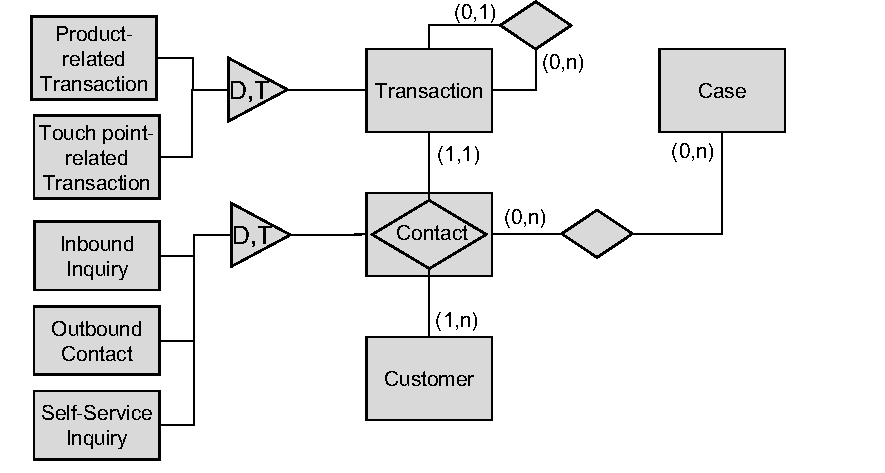
\includegraphics[width=.8\textwidth]{figures/contacterm.pdf}}
	 \end{figure} 
	 
	 
	 This analysis is necessary due to the complex and highly variable processes in Customer Service. Process Identification for Customer Service in the field of the After Sales Service as a Basis for “Lean After Sales Service”
	 im hippner buch it automation chapter für self service!
	 %%%%%%%%%%
	 Self Service: Servitization paper 1988!
	 
	 hippner:692 muss nicht nur inbound sein, outbound geht auch
	 
	 \subsection{Inbound}
	 The associated object to this process in the \textit{inquiry}\footnote{inquiry is American English; enquiry is British English.}. It is preferred over \textit{request} as it emphasizes an investigation in an issue over the politeness during asking. It is defined as an act of asking for information \citep{oxfordenquiry, oxfordrequest}. In this case, it is the customer who is lacking information in some regard and contacts the company. A \acrshort{CSR} of the outsourcing provider attends to the matter. 
	 
	 Reflections on the structure of the process become especially important in case of an omni-channel environment. There are multiple contact channels, asynchronous and synchronous communication and generic reasons that lead to the inquiry. Rationale behind omni-channel process modeling must be to keep the structure channel independent as long as possible to enable alignment. To capture the peculiarities of the channels, the concept of variants is used on the lowest level to distinguish between mail, voice, direct messenger and social channels. Reasons for this split is that other discussed channels (Video, Website, App) can be included in others by means of a process view (video to voice) or are not a contact channel by means of inbound customer service. The website and app are gateways to other channels (direct messenger) or to self-service, but do not offer direct engagement with a \acrshort{CSR}. Variants can be added, so that other channels can be easily added to the model. While there are similarities between (a)synchronous channels, using these as variants forecloses capturing of channel idiosyncrasies, because the underlying process building blocks would be the same for a variant. 
	 
	 The detail processes are structured so that their steps apply to all channels. This structuring was found to be applicable among the participants in the process modeling workshop and is shown in \Fig \ref{fig:inbproc}. First, the detail processes are described without going into details of their channel-variants. 
	 
	 \begin{figure}[caption={Inbound service process}, label={fig:inbproc}]
	 	\begin{subfigure}[b]{.45\textwidth}
	 		\begin{center}
	 			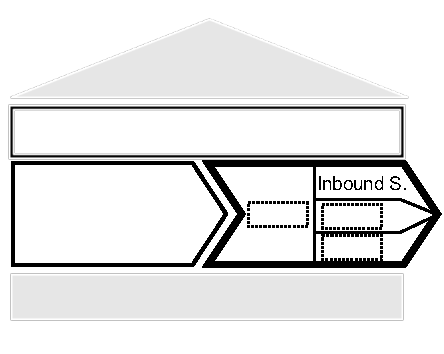
\includegraphics{figures/processes/inbound.pdf}
	 		\end{center}
	 	\end{subfigure}
	 	\begin{subfigure}[b]{.45\textwidth}
	 		\begin{center}
	 			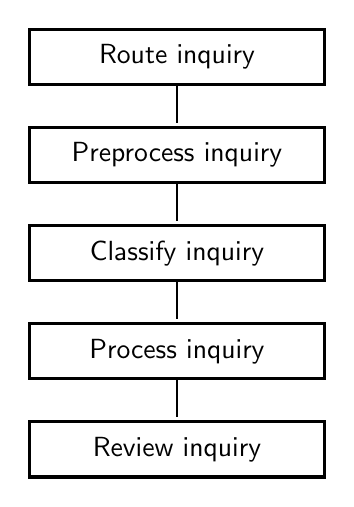
\begin{tikzpicture}
	 			[node distance=.5cm, start chain=going below,font=\sffamily]
	 			\node[punktchain, rounded corners=0pt, join=by {-}] (eins)      {Route inquiry};
	 			\node[punktchain, rounded corners=0pt, join=by {-}] (zwei) {Preprocess inquiry};
	 			\node[punktchain, rounded corners=0pt, join=by {-}, ] (drei) {Classify inquiry};
	 			\node[punktchain, rounded corners=0pt, join=by {-}, ] (vier) {Process inquiry};
	 			\node[punktchain,rounded corners=0pt,  join=by {-}, ] (fuenf) {Review inquiry};
	 			\end{tikzpicture}
	 		\end{center}
	 	\end{subfigure}
	 	
	 \end{figure}
	 
	 First, an inbound inquiry reaches is initiated by a customer and the connection with the receiving end is established. Before an interaction starts, the inquiry needs to be guided to a \acrshort{CSR}, which is known as routing in telecommunications. During this \textit{routing} process, information from the caller is processed, so that part of his needs can be inferred before the employee starts the conversation and time (and money) is consumed. On the other hand, time that the customer spends in the system before the conversation is not consuming scarce resources from the provider, so the pre-extraction of information usable to address his problem is desirable. At the end of routing, a \acrshort{CSR} is found that starts the conversation with the customer. In the \textit{preprocessing} step, the \acrshort{CSR} takes on the inquiry and consumes the information that is available from the routing, as well as transmitted by the customer. After this familiarization the \acrshort{CSR} can \textit{classify} the \textit{inquiry}, so that he knows how to map the individual inquiry of the customer to a case (if existent). The \textit{process inquiry} detail process engages the inquiry and ideally solves the problem. The last step involves a \textit{review} and closes the interaction. It updates data related to the communication and stores it in the knowledge base. As every detail process in \Fig \ref{fig:inbproc} has four variants, these are shown one by one in the following. 
	 
	 \subsubsection{Route Inquiry}
	 
	 Going into the specifics of the route inquiry detail process, \Fig \ref{fig:inbound:route} shows the four variants comprised of process building blocks. One can observe similarities 
	 across all variants, that especially in the beginning and end. During this step, no \acrshort{CSR} is actively involved.
	 \\
	 
	 \begin{figure}[caption={Route inquiry detail process}, label={fig:inbound:route}]
	 	
	 	\begin{subfigure}[b]{.45\textwidth}
	 		\centering
	 		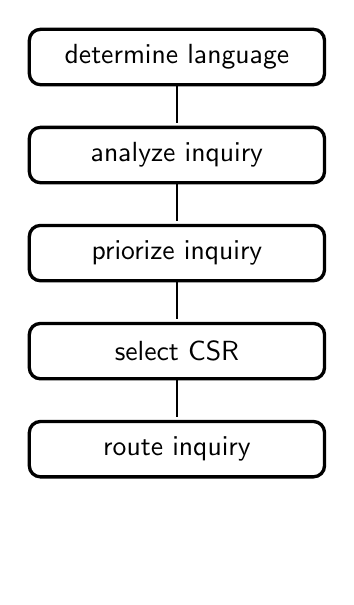
\begin{tikzpicture}
	 		[node distance=.5cm,
	 		start chain=going below,font=\sffamily]
	 		
	 		\node[punktchain, join=by {-}] (eins)      {determine language};
	 		\node[punktchain, join=by {-}] (zwei) {analyze inquiry};
	 		\node[punktchain, join=by {-}, ] (drei) {priorize inquiry};
	 		\node[punktchain, join=by {-}, ] (vier) {select CSR};
	 		\node[punktchain, join=by {-}, ] (fuenf) {route inquiry};
	 		\node[punktchain, draw=white] (sechs) { };
	 		
	 		\end{tikzpicture}
	 		
	 		\caption{Mail variant}\label{fig:inbound:route:mail}
	 	\end{subfigure}
	 	\begin{subfigure}[b]{.45\textwidth}
	 		\centering	
	 		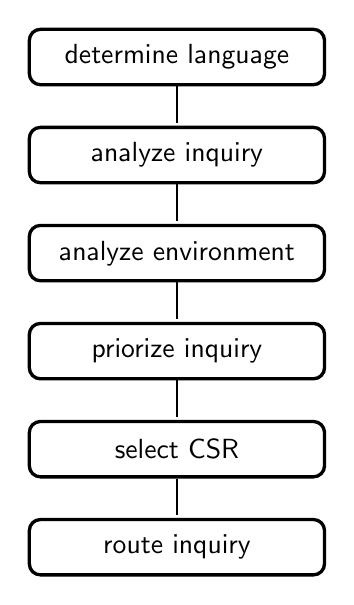
\begin{tikzpicture}
	 		[node distance=.5cm,
	 		start chain=going below,font=\sffamily]
	 		
	 		\node[punktchain, join=by {-}] (eins)      {determine language};
	 		\node[punktchain, join=by {-}] (zwei) {analyze inquiry};
	 		\node[punktchain, join=by {-}, ] (drei) {analyze environment};
	 		\node[punktchain, join=by {-}, ] (vier) {priorize inquiry};
	 		\node[punktchain, join=by {-}, ] (fuenf) {select CSR};
	 		\node[punktchain, join=by {-}, ] (sechs) {route inquiry};
	 		
	 		\end{tikzpicture}
	 		\caption{Social variant}\label{fig:inbound:route:social}
	 	\end{subfigure}
	 	\begin{subfigure}[b]{.45\textwidth}
	 		\centering	
	 		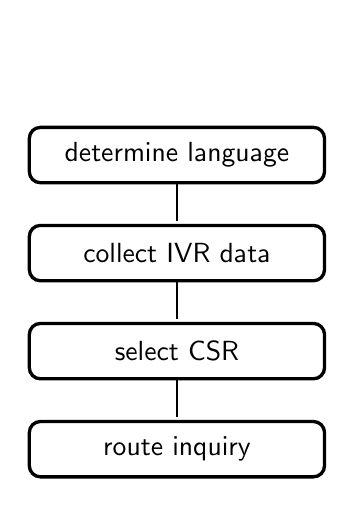
\begin{tikzpicture}
	 		[node distance=.5cm,
	 		start chain=going below,font=\sffamily]
	 		\node[punktchain, draw=white] (null) { };
	 		\node[punktchain] (eins)      {determine language};
	 		\node[punktchain, join=by {-}] (zwei) {collect IVR data};
	 		\node[punktchain, join=by {-}, ] (drei) {select CSR};
	 		\node[punktchain, join=by {-}, ] (vier) {route inquiry};
	 		
	 		\end{tikzpicture}
	 		\caption{Voice variant}\label{fig:inbound:route:voice}
	 	\end{subfigure}
	 	\begin{subfigure}[b]{.45\textwidth}
	 		\centering	
	 		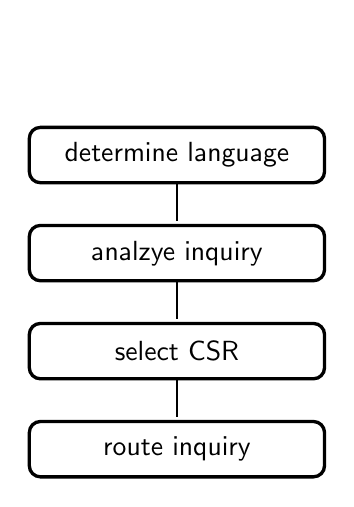
\begin{tikzpicture}
	 		[node distance=.5cm,
	 		start chain=going below,font=\sffamily]
	 		\node[punktchain, draw=white] (null) { };
	 		\node[punktchain] (eins)      {determine language};
	 		\node[punktchain, join=by {-}] (zwei) {analzye inquiry};
	 		\node[punktchain, join=by {-}, ] (drei) {select CSR};
	 		\node[punktchain, join=by {-}, ] (vier) {route inquiry};
	 		
	 		\end{tikzpicture}
	 		\caption{Direct Messenger variant}\label{fig:inbound:route:dm}
	 	\end{subfigure}
	 \end{figure}
	 
	 A common Language is a requirement for communication and needs to be known to understand the content of the inquiry. While this is required across channels, differences arise in the following step: All variants except voice can analyze the inquiry. This analysis uses available information from the inquiry, \ie its content or channel-specific data to identify the customer and infer the customer's need. In voice the inquiry itself is not existent at this point, as the customer has not expressed it verbally. However, \acrfull{IVR} technology helps to extract information from the customer without active involvement of a \acrshort{CSR} and is a typical technology in contact centers \citep{Thomas:2009}. The distinction between voice and the other variants is reasoned by the fact that the other inquiries are text-based and therefore analyzable by common means, which is not the case for voice. As \acrshort{IVR} is a standard in customer service, the naming of a explicit technology does not create conflicts in terms of universal applicability. The amount of information processed by it varies. Simple systems might just record input from the customer typed in via the phone keypad(\textit{if you have  a question regarding X, please press 2}), while sophisticated systems do natural language processing.
	 
	 The social variant includes an \textit{analyze environment} building block, which emphasizes the importance of the network's context in social media. The verb \textit{analyze} is again used to state automatism in this step. 
	 
	 Asynchronous channels (\ie, mail, social) have a \textit{priorize inquiry} step, that work around the \acrshort{FCFS} processing of inquiries. This step is not seen for synchronous channels, as the customer actively waits for a \acrshort{CSR} to take care of his inquiry. However, as the \textit{select  \acrshort{CSR}} step takes into account several aspects, it is not said that \acrshort{FCFS} applies to synchronous channels. The selection of the  \acrshort{CSR} depends on the requirements of the inquiry (\ie, language and to that point known content of the inquiry). Means to narrow down the variety content-wise is the availability of different contact channel instances. For example, there could be a dedicated mail address for reservations and another one for bookings. The fit of inquiry requirements to agent skills is known as skill-based routing. \acrshort{CSR}s can be clustered in agent groups that are the right contact person for the inquiry, so that additional rerouting is avoided. The last process building block models the actual routing of the inquiry, as now the receiving  \acrshort{CSR} is known. This can be done with an \acrfull{ACD} technology\footnote{Despite its naming, the technology is able to route calls of other channels \citep{ccn2016} } which is able to take available client and agent information into account.
	 
	 
	 \subsubsection{Preprocess Inquiry}
	 
	 This detail process, shown in \Fig \ref{fig:inbound:prepr}, begins with a \acrshort{CSR} entering the process, that consumes the available information of the inquiry. This is not possible on the voice channel. There, the agent needs to open the conversation first, followed by the listening to the customer. Then he obtains understanding of the problem and can checks whether the data form the \acrshort{IVR} is correct. The other channels, analogous to the route inquiry detail process, \textit{check analytical results} so that there is consensus of manually read inquiry content and analytically derived aspects.
	 
	 In the same way, the social variant includes a manual verification of the environment in the network. As elements can be skipped if not applicable (\ie no analytical system in place to check the environment in the social network), this building block may be interpreted as a first check of the environmental situation. Contextual factors (related posts with the same issue) on the facebook wall for instance may require a different approach towards the inquiry to ensure the appropriate reaction of the company in public.   
	 
	 The synchronous channels, \ie, \Fig \ref{fig:inbound:prepr:voice}, \ref{fig:inbound:prepr:dm} show time-logic differences. While the voice channel needs to open the conversation to know about the inquiry, a \acrshort{CSR} in a direct messenger communication is able to do the preprocessing step beforehand and opens the conversation to the customer at the end. 
	 
	 \begin{figure}[caption={Preprocess inquiry detail process}, label={fig:inbound:prepr}]
	 	
	 	\begin{subfigure}[b]{.45\textwidth}
	 		\centering
	 		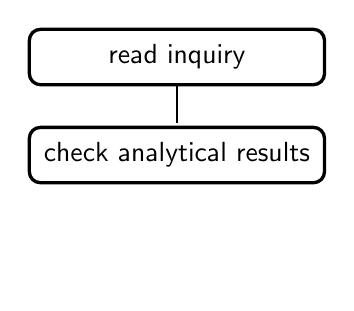
\begin{tikzpicture}
	 		[node distance=.5cm,
	 		start chain=going below,font=\sffamily]
	 		
	 		\node[punktchain, join=by {-}] (eins)      {read inquiry};
	 		\node[punktchain, join=by {-}] (zwei) {check analytical results};
	 		\node[punktchain,  draw=white,text=white] (sechs) {  verify environment};
	 		
	 		\end{tikzpicture}
	 		
	 		\caption{Mail variant}\label{fig:inbound:prepr:mail}
	 	\end{subfigure}
	 	\begin{subfigure}[b]{.45\textwidth}
	 		\centering	
	 		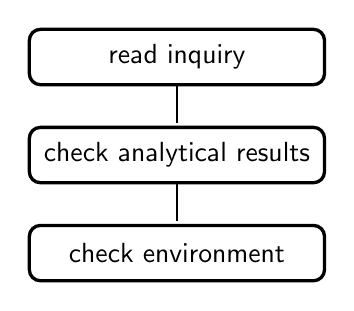
\begin{tikzpicture}
	 		[node distance=.5cm,
	 		start chain=going below,font=\sffamily]
	 		
	 		\node[punktchain, join=by {-}] (eins)      {read inquiry};
	 		\node[punktchain, join=by {-}] (zwei) {check analytical results};
	 		\node[punktchain, join=by {-}, ] (drei) {check environment};
	 		
	 		
	 		\end{tikzpicture}
	 		\caption{Social variant}\label{fig:inbound:prepr:social}
	 	\end{subfigure}
	 	\begin{subfigure}[b]{.45\textwidth}
	 		\centering	
	 		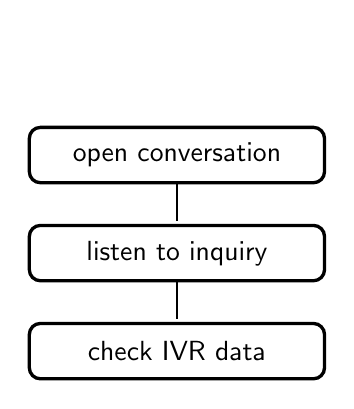
\begin{tikzpicture}
	 		[node distance=.5cm,
	 		start chain=going below,font=\sffamily]
	 		\node[punktchain, draw=white] (null) { };
	 		\node[punktchain] (eins)      {open conversation};
	 		\node[punktchain, join=by {-}] (zwei) {listen to inquiry};
	 		\node[punktchain, join=by {-}, ] (drei) {check IVR data};
	 		
	 		
	 		\end{tikzpicture}
	 		\caption{Voice variant}\label{fig:inbound:prepr:voice}
	 	\end{subfigure}
	 	\begin{subfigure}[b]{.45\textwidth}
	 		\centering	
	 		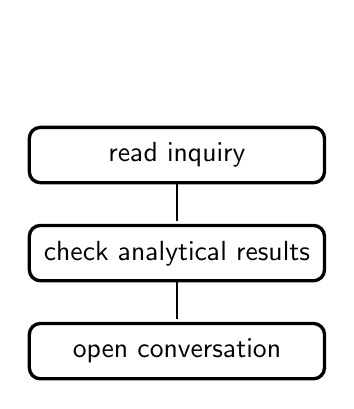
\begin{tikzpicture}
	 		[node distance=.5cm,
	 		start chain=going below,font=\sffamily]
	 		\node[punktchain, draw=white] (null) { };
	 		\node[punktchain] (zwei) {read inquiry};
	 		\node[punktchain, join=by {-}, ] (drei) {check analytical results};
	 		\node[punktchain, join=by {-}, ] (vier) {open conversation};
	 		
	 		\end{tikzpicture}
	 		\caption{Direct Messenger variant}\label{fig:inbound:prepr:dm}
	 	\end{subfigure}
	 \end{figure}
	 
	 
	 \subsubsection{Classify Inquiry}
	 
	 \Fig \ref{fig:inbound:class} shows the four variants for the third detail process of the inbound process. One can see that there is no difference seen between asynchronous (top row) and synchronous (lower row), so it is possible to shrink the representation down to two variants or even one variant, as the \textit{request missing information} building block can be skipped in the icebricks language if not applicable. For the sake of consistency across all detail processes, the four variant split is preserved.
	 
	 \begin{figure}[caption={Classify inquiry detail process}, label={fig:inbound:class}]
	 	
	 	
	 	\begin{subfigure}[b]{.45\textwidth}
	 		\centering
	 		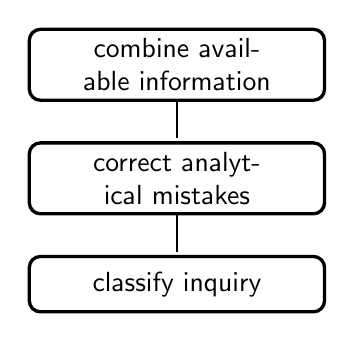
\begin{tikzpicture}
	 		[node distance=.5cm,
	 		start chain=going below,font=\sffamily]
	 		
	 		\node[punktchain, join=by {-}] (eins)      {combine available information};
	 		\node[punktchain, join=by {-}] (zwei) {correct analytical mistakes};
	 		\node[punktchain, join=by {-}] (drei) {classify inquiry};
	 		
	 		
	 		\end{tikzpicture}
	 		
	 		\caption{Mail variant}\label{fig:inbound:class:mail}
	 	\end{subfigure}
	 	\begin{subfigure}[b]{.45\textwidth}
	 		\centering	
	 		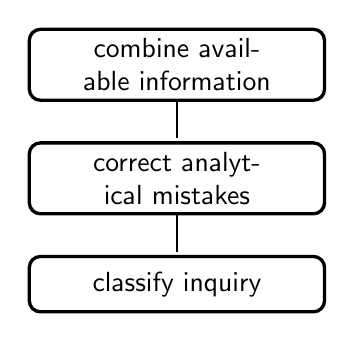
\begin{tikzpicture}
	 		[node distance=.5cm,
	 		start chain=going below,font=\sffamily]
	 		
	 		\node[punktchain, join=by {-}] (eins)      {combine available information};
	 		\node[punktchain, join=by {-}] (zwei) {correct analytical mistakes};
	 		\node[punktchain, join=by {-}] (drei) {classify inquiry};
	 		
	 		\end{tikzpicture}
	 		\caption{Social variant}\label{fig:inbound:class:social}
	 	\end{subfigure}
	 	\begin{subfigure}[b]{.45\textwidth}
	 		\centering	
	 		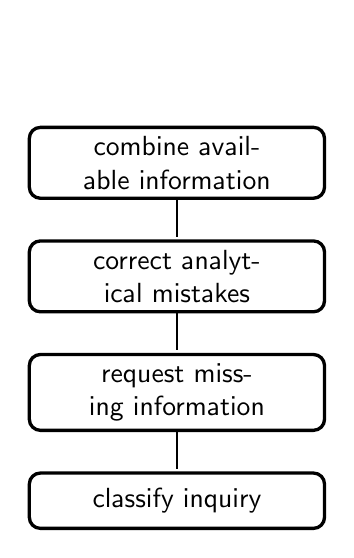
\begin{tikzpicture}
	 		[node distance=.5cm,
	 		start chain=going below,font=\sffamily]
	 		\node[punktchain, draw=white] (null) { };
	 		\node[punktchain] (eins)      {combine available information};
	 		\node[punktchain, join=by {-}] (zwei) {correct analytical mistakes};
	 		\node[punktchain, join=by {-}] (drei) {request missing information};
	 		\node[punktchain, join=by {-}] (vier) {classify inquiry};
	 		
	 		
	 		\end{tikzpicture}
	 		\caption{Voice variant}\label{fig:inbound:class:voice}
	 	\end{subfigure}
	 	\begin{subfigure}[b]{.45\textwidth}
	 		\centering	
	 		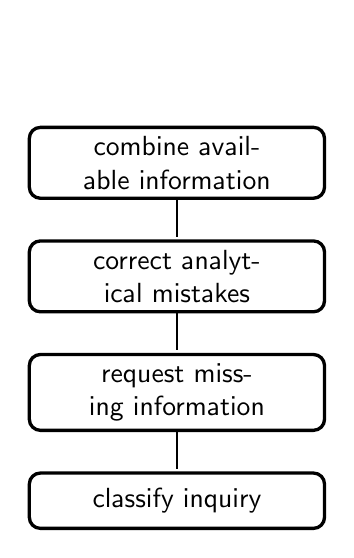
\begin{tikzpicture}
	 		[node distance=.5cm,
	 		start chain=going below,font=\sffamily]
	 		\node[punktchain, draw=white] (null) { };
	 		\node[punktchain] (eins)      {combine available information};
	 		\node[punktchain, join=by {-}] (zwei) {correct analytical mistakes};
	 		\node[punktchain, join=by {-}] (drei) {request missing information};
	 		\node[punktchain, join=by {-}] (vier) {classify inquiry};
	 		
	 		\end{tikzpicture}
	 		\caption{Direct Messenger variant}\label{fig:inbound:class:dm}
	 	\end{subfigure}
	 \end{figure}
	 
	 First, the available information of the inquiry and the analytical support from the two previous detail processes is combined to form one understanding of the inquiry for the \acrshort{CSR}. Next, mistakes of the analytical support are corrected, so that the system gets feedback and may improve in future.
	 
	 Third, the \textit{ classify inquiry} building block connects the inquiry (up to here seen as an instantiation of an unknown case) to a class. This class is a known construct in the mind of the \acrfull{CSR} and ideally described in a knowledge base as a case. An example for this split is an inquiry by a customer a, that expresses his wish to swap his ticket of x on day y to day z. The \acrshort{CSR} can classify this inquiry as class \textit{change of booking}. With this link being established, the problem is understood by the  \acrshort{CSR} and inquiry processing can be commenced. 
	 
	 Synchronous channels contain a \textit{request additional information} building block, that enables the \acrshort{CSR} to get additional information from the customer needed prior to classification(a booking number is required for a change of booking and not known). This is put before classification, so that a class can have requirements that need to be fulfilled before assignment. By this logic, the \acrshort{CSR} needs to have a guess about the customer's need, so that the right information is requested.  
	 
	 This classification of the inquiry, \ie, the mapping of the customers individually expressed needs to a modeled case on company/provider-side is seen as the essential task of the \acrshort{CSR} here. If the case was correctly modeled and identified, in theory its process would be adequately represented by \acrshort{IS} and no human involvement from the customer service side would be necessary. 
	 
	 \subsubsection{Process Inquiry}
	 
	 The process inquiry detail process is shown in \Fig \ref{fig:inbound:proc}. It represents the addressing of the customer need, that was previously defined and classified. Similarities among all variants are the starting building block \textit{query knowledge base}. This models the \acrshort{CSR}'s lookup of information related to the case at hand, either to give the requested information to the customer or to look up the process to solve the customer's issue.  
	 
	 Asynchronous channels, \Fig \ref{fig:inbound:proc:mail}, \ref{fig:inbound:proc:social}, contain a \textit{draft response} building block. Draft is used to enable the possibility of a following review step. Response on the other hand represents the asynchronous property of the communication. The response to the inquiry does not necessarily solve the customer's problem, as no conversation is included that verifies the correct understanding of the problem. Synchronous channels are assumed to solve the inquiry within the bounds of possibility. 
	 
	 The models on the right side of \Fig \ref{fig:inbound:proc} both contain a \textit{check-privacy guidelines} and \textit{request channel switch} building block. As direct messengers or social networks are often platforms, operated by other parties that may have a different understanding of data privacy, certain business cases cannot be processed on these channels. Hence, a channel switch becomes necessary and ends the process. 
	 
	 The voice channel additionally includes an identification segment, that represents the \acrshort{CSR}s ability to verify the customer's identity during the conversation. This does not represent the identification of the customer to an entry in the \acrshort{CRM} database, but a legally binding statement, that may be required for certain business cases. Video communication is a means to achieve the certainty of identity for the \acrshort{CSR}.
	 A channel like mail lacks the ability to identify a customer, as everyone with access to the customer's account can send on his behalf. This represents knowledge at the time of writing based on current practice. In future, a legally binding identification over different channels might be possible, for example via social media profile.
	 
	 
	 \begin{figure}[caption={Process inquiry detail process}, label={fig:inbound:proc}]
	 	
	 	\begin{subfigure}[b]{.45\textwidth}
	 		\centering
	 		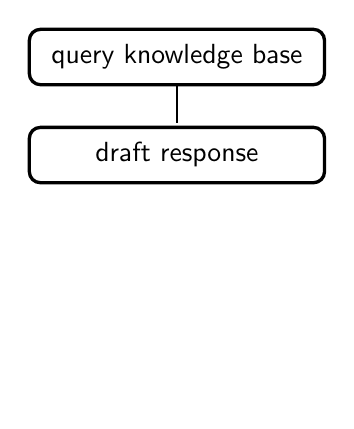
\begin{tikzpicture}
	 		[node distance=.5cm,
	 		start chain=going below,font=\sffamily]
	 		
	 		\node[punktchain, join=by {-}] (eins)      {query knowledge base};
	 		\node[punktchain, join=by {-}] (zwei) {draft response};
	 		\node[punktchain, text=white,draw=white] (drei) {request missing information};
	 		\node[punktchain, text=white,draw=white] (vier) {classify inquiry};
	 		
	 		
	 		\end{tikzpicture}
	 		
	 		\caption{Mail variant}\label{fig:inbound:proc:mail}
	 	\end{subfigure}
	 	\begin{subfigure}[b]{.45\textwidth}
	 		\centering	
	 		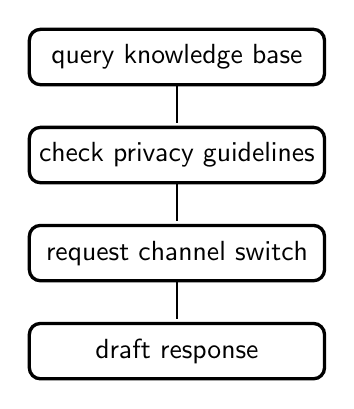
\begin{tikzpicture}
	 		[node distance=.5cm,
	 		start chain=going below,font=\sffamily]
	 		
	 		\node[punktchain, join=by {-}] (eins)      {query knowledge base};
	 		\node[punktchain, join=by {-}] (zwei) {check privacy guidelines};
	 		\node[punktchain, join=by {-}] (drei) {request channel switch};
	 		\node[punktchain, join=by {-}] (vier) {draft response};
	 		
	 		\end{tikzpicture}
	 		\caption{Social variant}\label{fig:inbound:proc:social}
	 	\end{subfigure}
	 	\begin{subfigure}[b]{.45\textwidth}
	 		\centering	
	 		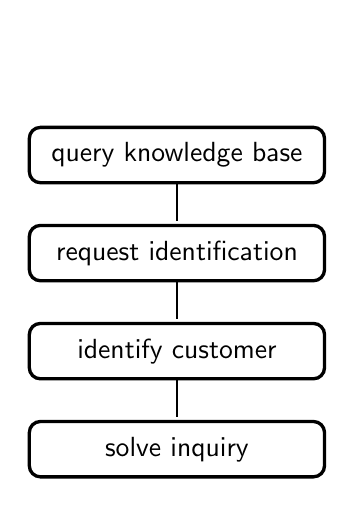
\begin{tikzpicture}
	 		[node distance=.5cm,
	 		start chain=going below,font=\sffamily]
	 		\node[punktchain, draw=white] (null) { };
	 		\node[punktchain] (eins)      {query knowledge base};
	 		\node[punktchain, join=by {-}] (zwei) {request identification};
	 		\node[punktchain, join=by {-}] (drei) {identify customer};
	 		\node[punktchain, join=by {-}] (vier) {solve inquiry};
	 		
	 		
	 		\end{tikzpicture}
	 		\caption{Voice variant}\label{fig:inbound:proc:voice}
	 	\end{subfigure}
	 	\begin{subfigure}[b]{.45\textwidth}
	 		\centering	
	 		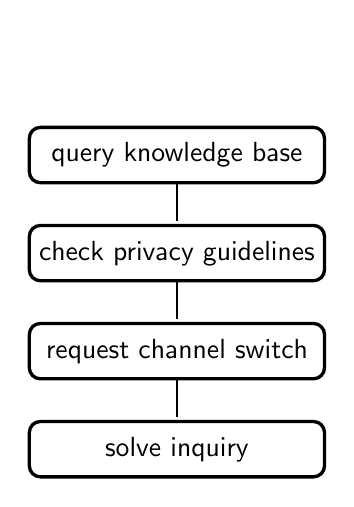
\begin{tikzpicture}
	 		[node distance=.5cm,
	 		start chain=going below,font=\sffamily]
	 		\node[punktchain, draw=white] (null) { };
	 		\node[punktchain] (eins)      {query knowledge base};
	 		\node[punktchain, join=by {-}] (zwei) {check privacy guidelines};
	 		\node[punktchain, join=by {-}] (drei) {request channel switch};
	 		\node[punktchain, join=by {-}] (vier) {solve inquiry};
	 		
	 		\end{tikzpicture}
	 		\caption{Direct Messenger variant}\label{fig:inbound:proc:dm}
	 	\end{subfigure}
	 \end{figure}
	 
	 
	 \subsubsection{Review Inquiry}
	 \label{inb:review}
	 Review inquiry is the last detail process within the inbound process. Its four variants can be inspected in \Fig \ref{fig:inbound:revw}. Two meanings of the notion of review in the Oxford Dictionary \citep{oxfordreview} fit to explain the different variants. First, a review is a \enquote{formal assessment of something with the intention of instituting change if necessary}. This definition fits to describe building blocks in asynchronous channels mail and social. A \acrshort{CSR} might need to send a response to a supervisor for checking. The supervisor can change parts or approve it directly (called \textit{finalize} here). In social networks, the environment should be checked again, as it could have changed since compilation of the draft. Also, the submission of the response is called \textit{posting} to emphasize differences of public posting to private \textit{sending} of mails.
	 
	 Synchronous channels (\cf \Fig \ref{fig:inbound:revw:voice}, \ref{fig:inbound:revw:dm}) show the same components, that are again not aggregated into one variant for consistency reasons. As they solve the inquiry during the synchronous conversation, no review according to the given definition is possible. However, second meaning of the term review explains the purpose of this step: \enquote{A report on or evaluation of a subject or past events}. 
	 
	 This justifies the last two process building blocks of all three variants, namely \textit{update customer data} and \textit{update inquiry}. As the interaction is completed at this point (\viz the response is sent, posted and the synchronous conversation is closed), information from the customer contact is to be stored. On the one hand, the customer contact, seen as a touch point and therefore a transaction, is connected to the customer in the \acrshort{CRM} data base. Additional data that might be revealed during the contact can also be stored to enrich the profile by the \acrshort{CSR}. Furthermore, the inquiry itself can be updated to keep track of the customer's issue if not solved entirely. Ticket systems are a concept to model this matter. The system itself  keeps track of handling times and other measures of the inquiry, so that data for reporting is generated. 
	 
	 
	 \begin{figure}[caption={Review inquiry detail process}, label={fig:inbound:revw}]
	 	
	 	\begin{subfigure}[b]{.45\textwidth}
	 		\centering
	 		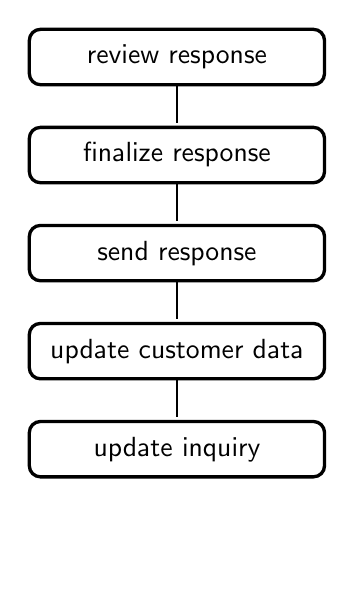
\begin{tikzpicture}
	 		[node distance=.5cm,
	 		start chain=going below,font=\sffamily]
	 		
	 		\node[punktchain, join=by {-}] (eins)      {review response};
	 		\node[punktchain, join=by {-}] (zwei) {finalize response};
	 		\node[punktchain, join=by {-}] (drei) {send response};
	 		\node[punktchain, join=by {-}] (vier) {update customer data};
	 		\node[punktchain, join=by {-}] (fuenf) {update inquiry};
	 		\node[punktchain, draw=white,text=white] (sechs) {verify environment};
	 		
	 		\end{tikzpicture}
	 		
	 		\caption{Mail variant}\label{fig:inbound:revw:mail}
	 	\end{subfigure}
	 	\begin{subfigure}[b]{.45\textwidth}
	 		\centering	
	 		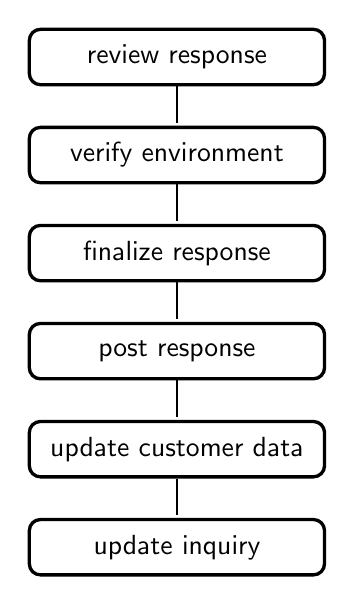
\begin{tikzpicture}
	 		[node distance=.5cm,
	 		start chain=going below,font=\sffamily]
	 		
	 		\node[punktchain, join=by {-}] (eins)      {review response};
	 		\node[punktchain, join=by {-}] (zwei) {verify environment};
	 		\node[punktchain, join=by {-}] (drei) {finalize response};
	 		\node[punktchain, join=by {-}] (vier) {post response};
	 		\node[punktchain, join=by {-}] (fuenf) {update customer data};
	 		\node[punktchain, join=by {-}] (sechs) {update inquiry};
	 		
	 		\end{tikzpicture}
	 		\caption{Social variant}\label{fig:inbound:revw:social}
	 	\end{subfigure}
	 	\begin{subfigure}[b]{.45\textwidth}
	 		\centering	
	 		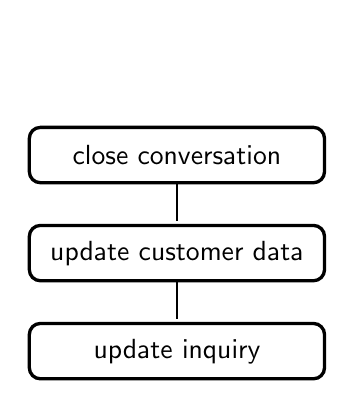
\begin{tikzpicture}
	 		[node distance=.5cm,
	 		start chain=going below,font=\sffamily]
	 		\node[punktchain, draw=white] (null) { };
	 		\node[punktchain] (eins)      {close conversation};
	 		\node[punktchain, join=by {-}] (zwei) {update customer data};
	 		\node[punktchain, join=by {-}] (drei) {update inquiry};
	 		\end{tikzpicture}
	 		\caption{Voice variant}\label{fig:inbound:revw:voice}
	 	\end{subfigure}
	 	\begin{subfigure}[b]{.45\textwidth}
	 		\centering	
	 		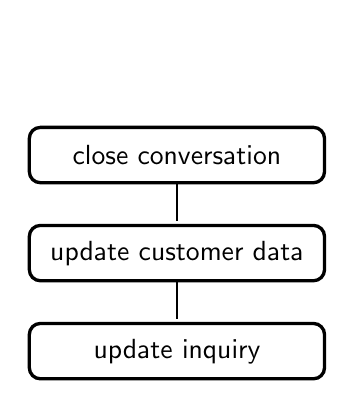
\begin{tikzpicture}
	 		[node distance=.5cm,
	 		start chain=going below,font=\sffamily]
	 		\node[punktchain, draw=white] (null) { };
	 		\node[punktchain] (eins) {close conversation};
	 		\node[punktchain, join=by {-}] (zwei) {update customer data};
	 		\node[punktchain, join=by {-}] (drei) {update inquiry};
	 		
	 		\end{tikzpicture}
	 		\caption{Direct Messenger variant}\label{fig:inbound:revw:dm}
	 	\end{subfigure}
	 \end{figure}
	 
	 
	 
	 
	 
	 
	 
	 
	 \subsection{Self-Service}
	 
	 The third customer interaction process leaves inter-personal service \citep{Thomas2008self} and focuses on ways that enable the customer to be the main value-generating part in the service interaction. This is facilitated by a technological component which can relieve the customer of a varying extent of the problem. The following illustrates this continuum from a customer perspective: Simple self-services, like an \acrshort{FAQ} section offer answers to questions, which the customer has to select from a list. The customer must express the need, map it to the available information, select the appropriate answer and process its content. A more advanced self-service might be able to additionally support the customer by the expression of the need and takes care of the mapping by a textual input, which is a more natural way of communication. The textual is analyzed and algorithmically mapped to the most appropriate solution, which is then presented to the customer, who must consume its content and is hopefully satisfied. It is noted that both solutions address the customer's issue, but sophisticated \acrshort{IT} increases usability by an easier interface to the customer's issue and a computed provision of a solution. This addresses what \citep{Thomas2008self} names a minimal skill set, \viz the an increased usability decreases the minimal skill set that is required for use. 
	 
	 From literature \citep{meuter2000self, Thomas2008self, Thomas:2009}, one can identify characteristics of self-services, which need to be considered in a process. As in the model the perspective of the service provider is chosen, the process needs to hold aspects which are seen from a system perspective. The previous example features the differences between a simple and technological enhanced serf-service. In both cases, the system has to provide information, but the simple self-services required the capability to express the need in the language of the service system, while the second allowed the customer to express it more naturally. The system perspective implies that the more active the customer takes the part in the process (\ie the simpler the self-service is), the less parts of the process are carried out by the system. 
	 
	 Furthermore, a self-service can be seen as part of a another customer service process. One can think of a self-service as support for a inter-personal contact, when it provides solutions based on customer information. Examples for this are \acrshort{IVR} or generated chat messages based on customer input.
	 
	 Unlike inter-personal services, self-services cannot be structured \wrt a communication channel, as they can be part of a service within one or multiple channels, or stand-alone in a web-based setting. A process representation is chosen which models both a supporting self-service for other services and a stand-alone implementation.
	 
	 \begin{figure}[caption={Self-Service process}, label={fig:selfservice}]
	 	\begin{subfigure}[b]{.45\textwidth}
	 		\begin{center}
	 			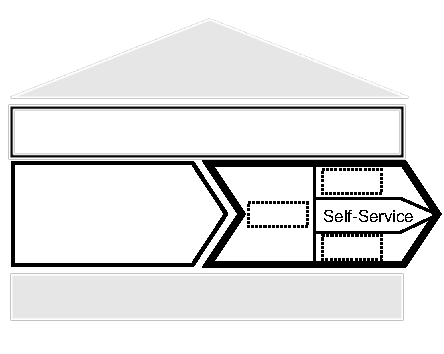
\includegraphics{figures/processes/selfservice.pdf}
	 		\end{center}
	 	\end{subfigure}
	 	\begin{subfigure}[b]{.45\textwidth}
	 		\begin{center}
	 			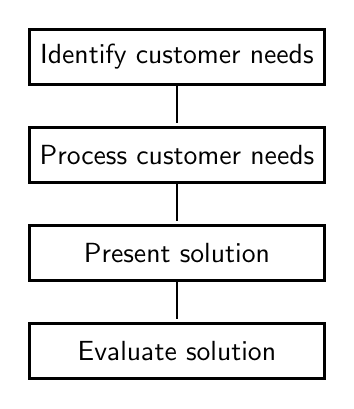
\begin{tikzpicture}
	 			[node distance=.5cm, start chain=going below,font=\sffamily]
	 			\node[punktchain, rounded corners = 0pt, join=by {-}] (eins)      {Identify customer needs};
	 			\node[punktchain,  rounded corners = 0pt,  join=by {-}] (zwei) {Process customer needs};
	 			\node[punktchain,  rounded corners = 0pt, join=by {-}, ] (drei) {Present solution};
	 			\node[punktchain, rounded corners = 0pt,  join=by {-}, ] (vier) {Evaluate solution};
	 			
	 			\end{tikzpicture}
	 		\end{center}
	 	\end{subfigure}
	 	
	 \end{figure}
	 
	 The process object customer need is chosen over inquiry to express the differences over inbound processing. It is noted that a customer need is an abstract construct that is used to express the customer's intention of use. However, like the inbound process self-service gets input from a customer and tries to solve the issue. But as there is no \acrshort{CSR} directly involved, there is less certainty that the system adequately addresses the \enquote{inquiry}. Due to this lack of a human counterpart on provider side, the technological interface provided by the system to the customer takes an important part in \textit{identifying customer needs}. As the capabilities of this interface vary drastically among different self-service scenarios, customer needs are chosen to emphasize the difference to inbound processing. \textit{Process customer needs} then aims at mapping the identified need to a defined solution in the knowledge base. After creation, \textit{present solution} communicates the findings to the customer. Lastly, \textit{evaluate solution} represents post-processing activities. The process is shown in \Fig \ref{fig:selfservice}.
	 
	 The building blocks of the four detail processes are summarized in \Fig \ref{fig:selfservice:detail}, as their is no further split into variants. The following description emphasizes the differences in simple and advanced self-service scenarios. 
	 
	 The building blocks of \textit{identfiy customer needs} (\Fig \ref{fig:selfservice:1}) capture external circumstances, that might be processed by the system to have more data available for inferring the customer need. Environmental factors are implicitly collected, \ie the customer does not need to state them. Request information models the input that the customer gives to the system. While the active phrasing might fit to more advanced self-service systems better than to simple \acrshort{FAQ}s, as the latter hardly asks the customer for information, the step applies to the concept of self-services: in order to narrow down the customer needs, relevant information needs to be selected by the customer (in a simple self-service system) or demanded as input for the system (in the advanced case). The verb \textit{infer} is used to describe the stochastic component of the system's attempt to understand the customer need. Again, the selection of a \acrshort{FAQ} entry by the customer might minimize the system's influence, still it conceives the selection as an information input and infers that the customer is \textit{needing} answers in this regard. An increased usability in the technological interface (arbitrary text input instead of a selection of options) also increases uncertainty in need identification, because the system has to select the fitting case by itself. 
	 
	 After the customer needs are inferred and hence available in a manner that corresponds to the data available in the knowledge base, the \textit{process customer needs} detail process (\Fig \ref{fig:selfservice:2}) receives  suitable information and creates a solution based on it. The solution represents the appropriate response to the customer's need. This can be the needed information, so that the need is completely addressed. Another option is that the self-service system can identify the need, but solving it requires personal-interaction. This expresses the limitations of service automation. 
	 
	 \textit{Present solution} (\Fig \ref{fig:selfservice:3}) conveys the result to the customer. The solution is presented by the system and is an adequate response to the customer's input. The customer's reaction is an important indicator of satisfaction and captured during the presentation. As the identification of a customer is not required for self-service use, these data needs to be stored in relation to the self-service input to further improve customer experience. The last detail process \textit{evaluate solution} (\Fig \ref{fig:selfservice:4}) can include a request for feedback (\enquote{Did this solve your problem?}) and finally all relevant information of the self-service use is stored and hence updates knowledge base. 
	 
	 \begin{figure}[caption={Self-service detail processes}, label={fig:selfservice:detail}]
	 	
	 	\begin{subfigure}[b]{.45\textwidth}
	 		\centering
	 		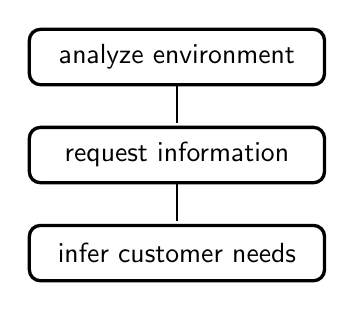
\begin{tikzpicture}
	 		[node distance=.5cm,
	 		start chain=going below,font=\sffamily]
	 		
	 		\node[punktchain, join=by {-}] (eins)      {analyze environment};
	 		\node[punktchain, join=by {-}] (zwei)      {request information};
	 		\node[punktchain, join=by {-}] (eins)      {infer customer needs};
	 		
	 		
	 		\end{tikzpicture}
	 		
	 		\caption{Identify customer needs}\label{fig:selfservice:1}
	 	\end{subfigure}
	 	\begin{subfigure}[b]{.45\textwidth}
	 		\centering	
	 		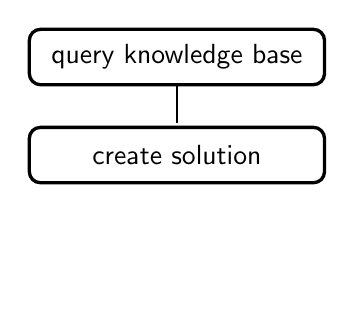
\begin{tikzpicture}
	 		[node distance=.5cm,
	 		start chain=going below,font=\sffamily]
	 		
	 		\node[punktchain, join=by {-}] (zwei) {query knowledge base};
	 		%	\node[punktchain, join=by {-}] (zwei) {integrate subsystem information};
	 		\node[punktchain, join=by {-}] (drei) {create solution};
	 		\node[punktchain, draw=white,text=white] (sechs) {verify environment};
	 		\end{tikzpicture}
	 		\caption{Process customer needs}\label{fig:selfservice:2}
	 	\end{subfigure}
	 	\begin{subfigure}[b]{.45\textwidth}
	 		\centering	
	 		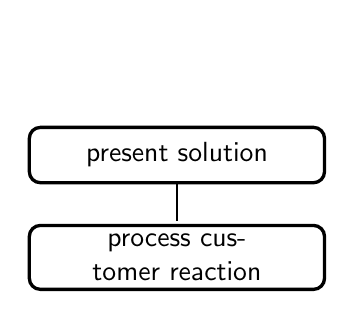
\begin{tikzpicture}
	 		[node distance=.5cm,
	 		start chain=going below,font=\sffamily]
	 		\node[punktchain, draw=white] (null) { };
	 		\node[punktchain] (eins)      {present solution};
	 		\node[punktchain, join=by {-}] (zwei) {process customer reaction};
	 		\end{tikzpicture}
	 		\caption{Present solution}\label{fig:selfservice:3}
	 	\end{subfigure}
	 	\begin{subfigure}[b]{.45\textwidth}
	 		\centering	
	 		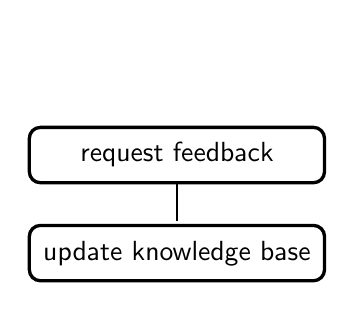
\begin{tikzpicture}
	 		[node distance=.5cm,
	 		start chain=going below,font=\sffamily]
	 		\node[punktchain, draw=white] (null) { };
	 		\node[punktchain] (eins) {request feedback};
	 		\node[punktchain, join=by {-}] (zwei) {update knowledge base};
	 		
	 		\end{tikzpicture}
	 		\caption{Evaluate solution}\label{fig:selfservice:4}
	 	\end{subfigure}
	 \end{figure}
	 
	 
	 
	 
	 klar definieren was ich unter sst verstehe \citep{Thomas:2009} hält auch online tech support boards, live chat sessions with customer support personal, user forums, etc. drin. also da wo der CSR noch supported. 
	 starting point \citep{Thomas:2009}.
	 %When a customer calls into the call center for technical support, it is often with the belief that they are contacting a CSR who is either an expert at solving their problem or at least more knowledgeable about their problem than the caller.
	 \citep{ccn2016} s.44
	 
	 %	To determine the most efficient, effective and mutually acceptable use of technology in service delivery, the customer's perspective needs to be known and understood.  \citep{Walker_2002}
	 
	 
	 \newpage
	 \newpage
	 
	 \subsection{Outbound Service}
	 
	 In contrast to inbound interactions that have an inquiry as central object of the process, the outreaching communications do not necessarily target a customer's issue. Its root depends on the purpose of the communication, which can be related to a previous interaction (call-back service in voice) or e-mail marketing (new offers via mail) for instance. Therefore, the general term \textit{contact} is used and defined as \enquote{a meeting, communication, or relationship with someone} \citep{oxfordcontact}. The verb refers to the communication with someone.
	 
	 Alike to inbound processing, omni-channel applicability is enabled by having a universal detail process, which has variants for each of the four contact channel categories. It is noted that outbound communication may apply differently across the channel types and dependent on implemented technology. There is the necessity of knowing the identifier of a customer within a contact channel to reach him. This identifier is the phone number in voice, mail address or a social media account. Direct messengers may be designed to enable use without individual sign-up, which excludes the ability to reach the customer. However, using direct messenger platforms such as WhatsApp enables outgoing communications, as work with identifiers. 
	 
	 \begin{figure}[caption={Outbound process}, label={fig:outbound}]
	 	\begin{subfigure}[b]{.45\textwidth}
	 		\begin{center}
	 			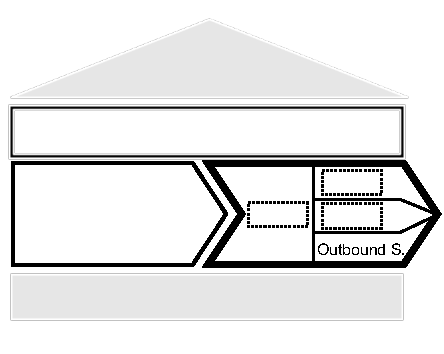
\includegraphics{figures/processes/outbound.pdf}
	 		\end{center}
	 	\end{subfigure}
	 	\begin{subfigure}[b]{.45\textwidth}
	 		\begin{center}
	 			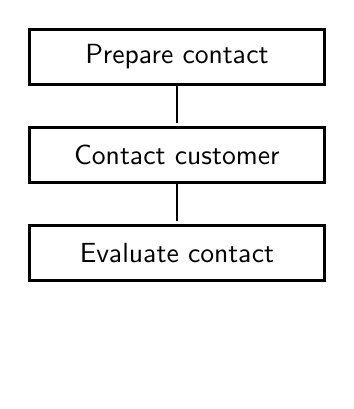
\begin{tikzpicture}
	 			[node distance=.5cm, start chain=going below,font=\sffamily]
	 			\node[punktchain,rounded corners=0pt, join=by {-}] (eins)      {Prepare contact};
	 			\node[punktchain,rounded corners=0pt, join=by {-}] (zwei) {Contact customer};
	 			\node[punktchain,rounded corners=0pt, join=by {-}, ] (drei) {Evaluate contact};
	 			\node[punktchain, draw=white ] (vier) { };
	 			
	 			\end{tikzpicture}
	 		\end{center}
	 	\end{subfigure}
	 	
	 \end{figure}
	 
	 
	 
	 
	 A fundamental difference the inbound and outbound process is that outbound contact is proactive and needs more initial information to act on, whereas inbound contact is more reactive \citep{DimensionData2015}. \Fig \ref{fig:outbound} shows the detail process, which is composed of three steps. As an analogy to the inbound detail process, the \textit{prepare contact} represents activities that take place prior to the activity that actually addresses the process object (route, preprocess, classify inquiry in the inbound process). The following \textit{contact customer} step expresses the active approach of the customer (contact) from the company side and can mirror the process inquiry step in the inbound process. Lastly, the \textit{evaluate contact} step contains subsequent efforts. Here the wording evaluate is chosen over review to put more focus on an assessment of the contact and less on the intention to change parts if necessary (\cf \ref{inb:review}). Furthermore, the company as contact initiator can perform a review at an earlier stage and does not need to react on a customer. 
	 
	 
	 \subsubsection{Prepare Contact}
	 
	 To actively approach a customer, there has to be a trigger or decision that lead to the initiation of the process, which is then assigned to the executing organizational unit, \ie \acrshort{CSR}. The information that captures the intention behind the contact is assumed to be stored in the knowledge base. The first step of this detail process (\Fig \ref{fig:outbound:prep}) is consequently a query to get the \acrshort{CSR} informed, which is consistent over all channel variants. Next, the aforementioned reason for contact is processed by the \acrshort{CSR} to enable the transfer of it towards the upcoming contact of the customer. 
	 
	 All channels except voice show three blocks, that also appear in the review inquiry inbound process variant (draft, review, finalize message/post). This early (optional) verification by a supervisor is possible because the communication is started by the company and the purpose is stored in the known reason for contact. Therefore, there is no processing of a customer inquiry necessary on which a response is formulated. Because of this, direct messengers can also have these component, even though it is a synchronous channel. In the voice variant, there is no review. The \acrshort{CSR} is assumed to understand the reason for contact or resolve any issues with it in the \textit{process reason for contact} step, as the scripting of a call is implausible. 
	 
	 The case of a proactive post of a company on a customer's social profile might seem less typical on platforms like facebook, but it cannot be foreclosed. In addition, it depends on the social behavior on the network that might change over time and varies across networks.  
	 
	 \begin{figure}[caption={Prepare contact detail process}, label={fig:outbound:prep}]
	 	
	 	\begin{subfigure}[b]{.45\textwidth}
	 		\centering
	 		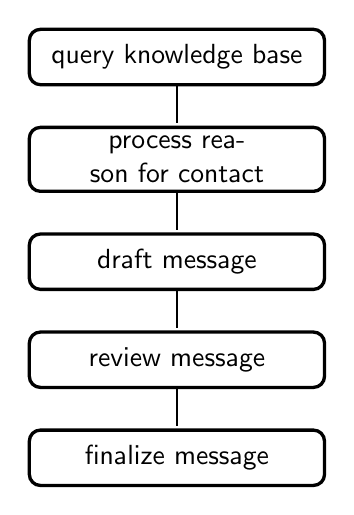
\begin{tikzpicture}
	 		[node distance=.5cm,
	 		start chain=going below,font=\sffamily]
	 		
	 		\node[punktchain, join=by {-}] (eins)      {query knowledge base};
	 		\node[punktchain, join=by {-}] (zwei) {process reason for contact};
	 		\node[punktchain, join=by {-}] (drei) {draft message};
	 		\node[punktchain, join=by {-}] (vier) {review message};
	 		\node[punktchain, join=by {-}] (fuenf) {finalize message};
	 		
	 		\end{tikzpicture}
	 		
	 		\caption{Mail variant}\label{fig:outbound:prep:mail}
	 	\end{subfigure}
	 	\begin{subfigure}[b]{.45\textwidth}
	 		\centering	
	 		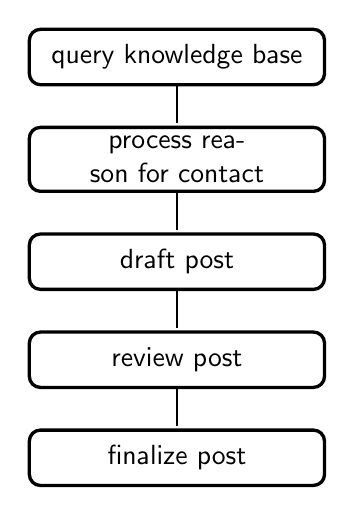
\begin{tikzpicture}
	 		[node distance=.5cm,
	 		start chain=going below,font=\sffamily]
	 		
	 		\node[punktchain, join=by {-}] (eins)      {query knowledge base};
	 		\node[punktchain, join=by {-}] (zwei) {process reason for contact};
	 		\node[punktchain, join=by {-}] (drei) {draft post};
	 		\node[punktchain, join=by {-}] (vier) {review post};
	 		\node[punktchain, join=by {-}] (fuenf) {finalize post};
	 		\end{tikzpicture}
	 		\caption{Social variant}\label{fig:outbound:prep:social}
	 	\end{subfigure}
	 	\begin{subfigure}[b]{.45\textwidth}
	 		\centering	
	 		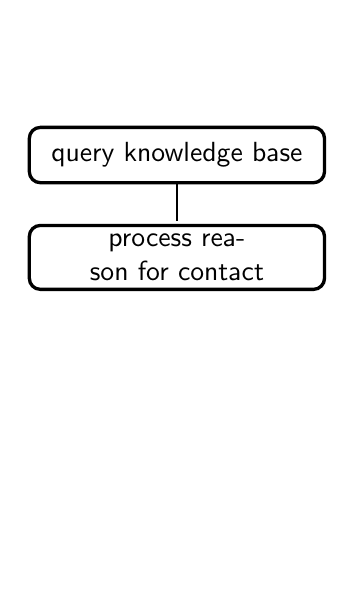
\begin{tikzpicture}
	 		[node distance=.5cm,
	 		start chain=going below,font=\sffamily]
	 		\node[punktchain, draw=white] (null) { };
	 		\node[punktchain] (eins)      {query knowledge base};
	 		\node[punktchain, join=by {-}] (zwei) {process reason for contact};
	 		\node[punktchain, draw=white] (null) { };
	 		\node[punktchain, draw=white] (null) { };
	 		\node[punktchain, draw=white] (null) { };
	 		
	 		\end{tikzpicture}
	 		\caption{Voice variant}\label{fig:outbound:prep:voice}
	 	\end{subfigure}
	 	\begin{subfigure}[b]{.45\textwidth}
	 		\centering	
	 		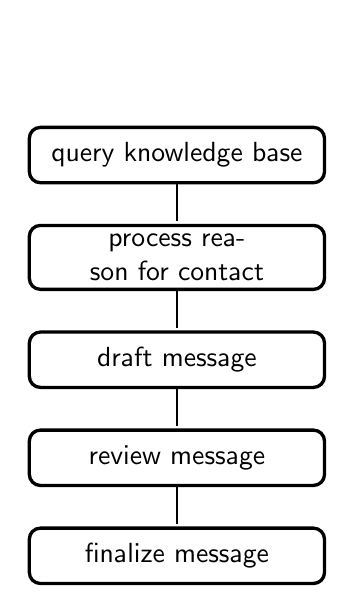
\begin{tikzpicture}
	 		[node distance=.5cm,
	 		start chain=going below,font=\sffamily]
	 		\node[punktchain, draw=white] (null) { };
	 		\node[punktchain] (eins) {query knowledge base};
	 		\node[punktchain, join=by {-}] (zwei) {process reason for contact};
	 		\node[punktchain, join=by {-}] (drei) {draft message};
	 		\node[punktchain, join=by {-}] (vier) {review message};
	 		\node[punktchain, join=by {-}] (fuenf) {finalize message};
	 		
	 		\end{tikzpicture}
	 		\caption{Direct Messenger variant}\label{fig:outbound:prep:dm}
	 	\end{subfigure}
	 \end{figure}
	 
	 
	 \subsubsection{Contact Customer}
	 
	 The second step of the outbound process models the approach of the client (\Fig \ref{fig:outbound:con}) . The use of contact as a verb expresses that the customer is on the receiving end. (A)synchronous channels show a similar structure, respectively. As the message or post is already prepared, the select of the sending account and the actual transmission\footnote{Theoretically, the second block in the social variant should be named \textit{post post}. Considering writing style, the object is kept and the verb changed to send. } is left. As previously justified, the variant in social media includes a verification step of the network environment. 
	 
	 Synchronous communication establishes a \textit{conversation} with the customer on which is responded in a timely manner. It is noted that in contrast to the voice channel, a direct message does not require the customer to respond directly to the \acrshort{CSR}s message. With this open connection, the  \acrshort{CSR} is able to \textit{communicate} the \textit{reason of contact} to the customer. 
	 
	 As the contact is initiated by the company, the customer might not understand the reason for contact properly. In this case of synchronous communication, it is possible for the \acrshort{CSR} to\textit{ solve complications} on the spot. The last block of the detail contact customer detail process encompasses the \textit{solving of }further \textit{questions}. Reason for this is that in the outbound case, there is object encapsulating the customer's need (as it is the inquiry in the inbound process). Ergo, the customer can have additional unresolved questions which can, but not necessarily have to, relate to the reason of contact. In analogy to the \textit{solve inquiry} block in inbound processing, the verb solve is again used to emphasize the activity of the  \acrshort{CSR}. 
	 
	 
	 \begin{figure}[caption={Contact customer detail process}, label={fig:outbound:con}]
	 	
	 	\begin{subfigure}[b]{.45\textwidth}
	 		\centering
	 		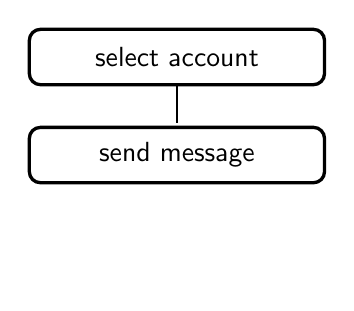
\begin{tikzpicture}
	 		[node distance=.5cm,
	 		start chain=going below,font=\sffamily]
	 		
	 		\node[punktchain, join=by {-}] (eins)      {select account};
	 		\node[punktchain, join=by {-}] (zwei) {send message};
	 		\node[punktchain, draw=white] (null) { };
	 		\end{tikzpicture}
	 		
	 		\caption{Mail variant}\label{fig:outbound:con:mail}
	 	\end{subfigure}
	 	\begin{subfigure}[b]{.45\textwidth}
	 		\centering	
	 		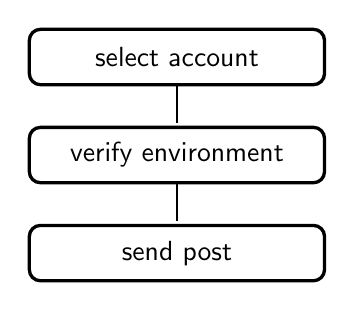
\begin{tikzpicture}
	 		[node distance=.5cm,
	 		start chain=going below,font=\sffamily]
	 		
	 		\node[punktchain, join=by {-}] (eins)      {select account};
	 		\node[punktchain, join=by {-}] (zwei) {verify environment};
	 		\node[punktchain, join=by {-}] (drei) {send post};
	 		\end{tikzpicture}
	 		\caption{Social variant}\label{fig:outbound:con:social}
	 	\end{subfigure}
	 	\begin{subfigure}[b]{.45\textwidth}
	 		\centering	
	 		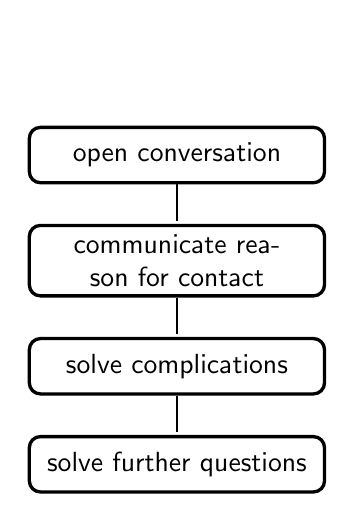
\begin{tikzpicture}
	 		[node distance=.5cm,
	 		start chain=going below,font=\sffamily]
	 		\node[punktchain, draw=white] (null) { };
	 		\node[punktchain] (eins)      {open conversation};
	 		\node[punktchain, join=by {-}] (zwei) {communicate reason for contact};
	 		\node[punktchain, join=by {-}] (drei) {solve complications};
	 		\node[punktchain, join=by {-}] (vier) {solve further questions};
	 		
	 		\end{tikzpicture}
	 		\caption{Voice variant}\label{fig:outbound:con:voice}
	 	\end{subfigure}
	 	\begin{subfigure}[b]{.45\textwidth}
	 		\centering	
	 		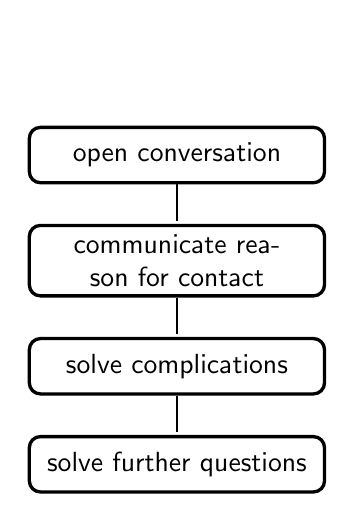
\begin{tikzpicture}
	 		[node distance=.5cm,
	 		start chain=going below,font=\sffamily]
	 		\node[punktchain, draw=white] (null) { };
	 		\node[punktchain] (eins)      {open conversation};
	 		\node[punktchain, join=by {-}] (zwei) {communicate reason for contact};
	 		\node[punktchain, join=by {-}] (drei) {solve complications};
	 		\node[punktchain, join=by {-}] (vier) {solve further questions};
	 		
	 		\end{tikzpicture}
	 		\caption{Direct Messenger variant}\label{fig:outbound:con:dm}
	 	\end{subfigure}
	 \end{figure}
	 
	 
	 
	 \subsubsection{Evaluate Contact}
	 
	 This detail process step (\Fig \ref{fig:outbound:eval}) closes the synchronous conversation and represents closing activities that are related to the contact. Synchronous channels close the conversation at the beginning, while asynchronous channels are completed with posting or sending. Mirrored from the inbound process, the process building blocks \textit{update customer data} and \textit{update contact} draw a line to the review inquiry process. Here, the inquiry object is replaced by the contact object. 
	 
	 \begin{figure}[caption={Evaluate contact detail process}, label={fig:outbound:eval}]
	 	
	 	\begin{subfigure}[b]{.45\textwidth}
	 		\centering
	 		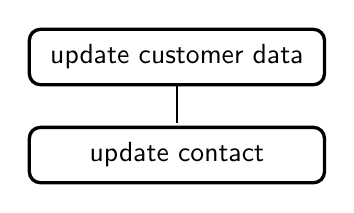
\begin{tikzpicture}
	 		[node distance=.5cm,
	 		start chain=going below,font=\sffamily]
	 		
	 		\node[punktchain, join=by {-}] (eins)      {update customer data};
	 		\node[punktchain, join=by {-}] (zwei) {update contact};
	 		\end{tikzpicture}
	 		
	 		\caption{Mail variant}\label{fig:outbound:eval:mail}
	 	\end{subfigure}
	 	\begin{subfigure}[b]{.45\textwidth}
	 		\centering	
	 		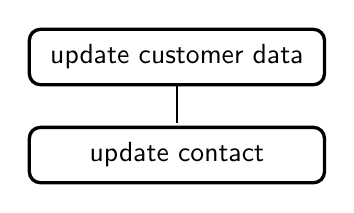
\begin{tikzpicture}
	 		[node distance=.5cm,
	 		start chain=going below,font=\sffamily]
	 		
	 		\node[punktchain, join=by {-}] (eins)      {update customer data};
	 		\node[punktchain, join=by {-}] (zwei) {update contact};
	 		\end{tikzpicture}
	 		\caption{Social variant}\label{fig:outbound:eval:social}
	 	\end{subfigure}
	 	\begin{subfigure}[b]{.45\textwidth}
	 		\centering	
	 		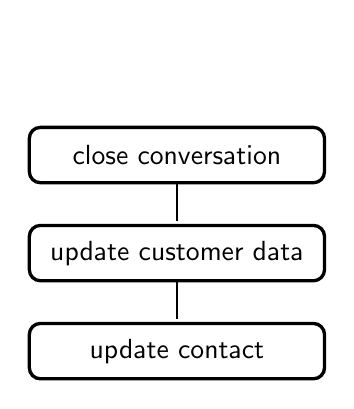
\begin{tikzpicture}
	 		[node distance=.5cm,
	 		start chain=going below,font=\sffamily]
	 		\node[punktchain, draw=white] (null) { };
	 		\node[punktchain] (eins)      {close conversation};
	 		\node[punktchain, join=by {-}] (zwei) {update customer data};
	 		\node[punktchain, join=by {-}] (drei) {update contact};
	 		
	 		
	 		\end{tikzpicture}
	 		\caption{Voice variant}\label{fig:outbound:eval:voice}
	 	\end{subfigure}
	 	\begin{subfigure}[b]{.45\textwidth}
	 		\centering	
	 		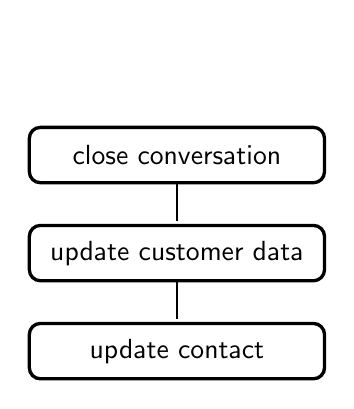
\begin{tikzpicture}
	 		[node distance=.5cm,
	 		start chain=going below,font=\sffamily]
	 		\node[punktchain, draw=white] (null) { };
	 		\node[punktchain] (eins)      {close conversation};
	 		\node[punktchain, join=by {-}] (zwei) {update customer data};
	 		\node[punktchain, join=by {-}] (drei) {update contact};
	 		
	 		\end{tikzpicture}
	 		\caption{Direct Messenger variant}\label{fig:outbound:eval:dm}
	 	\end{subfigure}
	 \end{figure}
	 
	 
	 
	 
	 \subsection{Knowledge Management}
	 

Knowledge management is a widely used term across different fields of academic research. \cite{girard2015defining} compile over 100 definitions and analyze their content. They propose to define it as \enquote{the process of creating, sharing, using and managing the knowledge and information of an organization\footnote{Organization refers to a client business in this case.}.} \citep[\p{14}]{girard2015defining} based on the most frequent words. It is noted that this definition can be criticized as too general, but it is chosen because it takes a process view and fits to the position in the framework: The interpretation as part of the customer-facing processes emphasizes the role of knowledge management in operative business. Hence, this view of knowledge management limits its boundaries to a certain client business. Knowledge management for the provider organization is seen as an important aspect, yet it encompasses various areas which are separated into distinct management processes. Therefore it is desisted from the creation of a global knowledge management process. The importance of knowledge management in operative business is stressed by its third rank regarding upcoming investments in contact centers \citep{ccnet2016}. 

Building on the previously proposed \acrshort{ERM} for customer-facing services (\ref{fig:contacterm}), a transaction, customer and case are entities that stand in relation to the customer contact. The latter represents the business object of the three services that form the interface to the customer. In these processes, the remaining transaction, customer and case entity become an integral component and shall be modeled as three variants of the main process. 

\acrshort{CSR}s need a source of information so that they can adequately perform the mapping of customer inquiries to organizational knowledge. When the cancellation of contract is requested by a customer, the \acrshort{CSR} can look up whether a case exists that contains the knowledge to satisfy the customer, \viz instructions for performing the cancellation in relevant systems. In a self-service scenario, the knowledge base is largely defining the capabilities of the service. 

Transactions capture events and are always connected to a customer. They relate to a product or a touch point and have a hierarchy: a purchase can be the result of a previous touch point (informing about its features for instance). This information is critical to uncover a customer journey and the more transactions are known, the better the \acrshort{CSR}'s understanding of the customer is. 

The customer as the focal point in \acrshort{CRM} and may or may not be known during a contact. When an identification can be performed, the knowledge base provides information regarding master data and transactions assigned to the entity. In order to achieve an omni-channel \acrshort{CRM} experience, the existence of a knowledge base about customers is critical for providing personalized services. 

Myriad frameworks try to distillate  the essence of knowledge management.  \cite{Rubenstein_Montano_2001} have examined various proposals and compared their similarities. Drawing on their analysis, activities in these frameworks serve as basis for the assessment of their applicability in the reference model. The omission of strategic frameworks narrows down the list. Frameworks that do not contain a procedural description are also excluded from further consideration. As several of the remaining frameworks show rather abstract and philosophical characteristics, the ones showing activities that can be understood from an \acrshort{IS} implementation perspective are selected. After evaluating the remaining four frameworks (\cf \ref{app:knowmang}), \citep{van_Heijst_1997} is chosen as a basis.

\citeauthor{van_Heijst_1997} list knowledge (1) development, (2) combination, (3) consolidation and (4) distribution as basic processes. They refer to the knowledge cycle in \citep{Wiig_1997}, where these are constituents of the \textit{act}-phases\footnote{The cycle contains four phases in total: conceptualize, reflect, act, review}. This placement fits well into the operative interpretation of knowledge management with the framework. 

Development is seen here as the acquisition of new knowledge  \citep{van_Heijst_1997} and the maintenance of the knowledge base. Combination uses the connection of different knowledge sources as a lever, which especially can gets important in the field of omni-channel \acrshort{CRM}. Consolidating signifies the processing of knowledge data so that it is available and usable. This relates one to one hand to analytical activities so that decisions can be based on aggregated data or \acrfull{KPI}s that provide decision-support. On the other hand, indexing and structuring of knowledge is necessary to facilitate fast access. This is important in manual access through \acrshort{CSR}s, as well as in the case of a self-service technology. Lastly, the distribution of knowledge describes the provision of knowledge to the organization. As the customer-facing processes show \textit{query knowledge base} as the active part of requesting, its counterpart is seen in this last process of knowledge management. 

In order to fit the three variants (case-related, customer-related, transaction-related) to these steps, the verbs \textit{maintain}, \textit{consolidate}, \textit{combine} and \textit{provide} are to represent the four processes of knowledge management. The object in the main process variants corresponds to the information that stands in center of the variant, which reasons the split so that distinct process building blocks can be added. For this thesis, only the textual description of the processes shall represent their content. There is no explicit modeling of the lowest layer of the framework. 

\begin{figure}[caption={Knowlege Management main process variants}, label={fig:knowledge}]
	\begin{subfigure}[b]{.6\textwidth}
		\begin{center}
			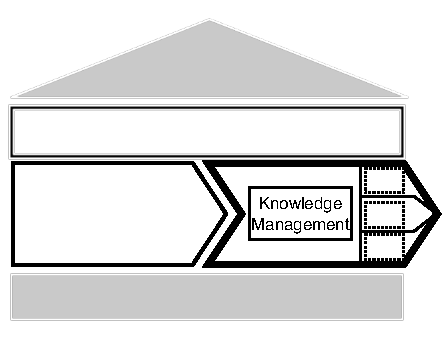
\includegraphics{figures/processes/knowledgemanagement.pdf}
		\end{center}
	\end{subfigure}

	\begin{subfigure}[b]{.32\textwidth}
		\begin{center}
			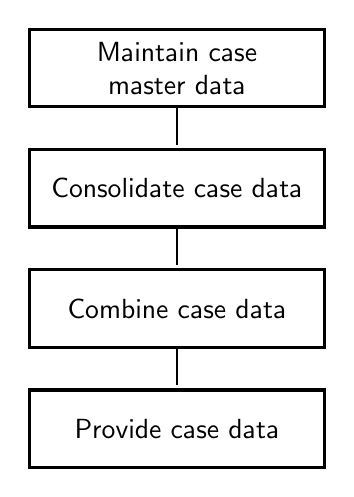
\begin{tikzpicture}
			[node distance=.5cm, minimum height=4.5em, start chain=going below,font=\sffamily]
			\node[punktchain, rounded corners=0pt , minimum height=2.8em,join=by {-}] (eins)      {Maintain case master data};
			\node[punktchain,rounded corners=0pt, minimum height=2.8em,  join=by {-}] (zwei) {Consolidate case data };
			\node[punktchain, rounded corners=0pt, minimum height=2.8em, join=by {-}, ] (drei) {Combine case data};
			\node[punktchain, rounded corners=0pt, minimum height=2.8em, join=by {-}, ] (vier) {Provide case data };

			\end{tikzpicture}
			\caption{Case-related variant}\label{fig:knowmang:case}
		\end{center}
	\end{subfigure}
\begin{subfigure}[b]{.32\textwidth}
	\begin{center}
		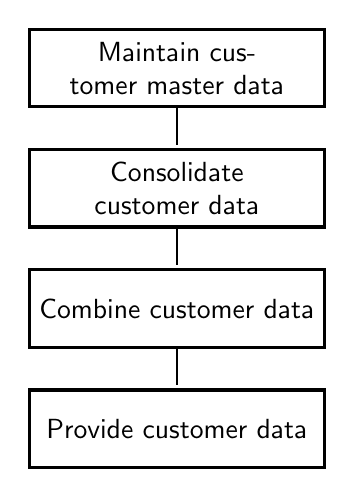
\begin{tikzpicture}
		[node distance=.5cm, start chain=going below,font=\sffamily]
		\node[punktchain, rounded corners=0pt, minimum height=2.8em,join=by {-}] (eins)      {Maintain customer master data};
		\node[punktchain,rounded corners=0pt,  
		minimum height=2.8em,join=by {-}] (zwei) {Consolidate customer data};
		\node[punktchain, rounded corners=0pt,  
		 minimum height=2.8em,join=by {-}, ] (drei) {Combine customer data};
		\node[punktchain, minimum height=2.8em, rounded corners=0pt, join=by {-}, ] (vier) {Provide customer data};
	
		\end{tikzpicture}
				\caption{Customer-related variant}\label{fig:knowmang:cust}
	\end{center}
\end{subfigure}
\begin{subfigure}[b]{.32\textwidth}
	\begin{center}
		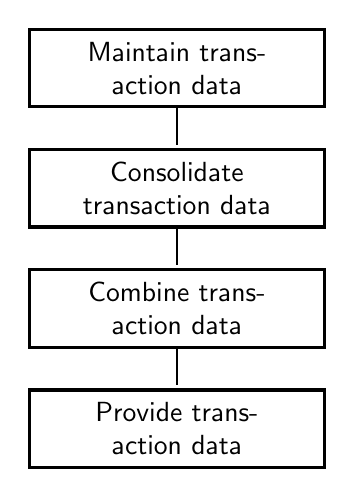
\begin{tikzpicture}
		[node distance=.5cm, start chain=going below,font=\sffamily]
		\node[punktchain, rounded corners=0pt,minimum height=2.8em ,join=by {-}] (eins)      {Maintain transaction data};
		\node[punktchain,rounded corners=0pt, minimum height=2.8em , join=by {-}] (zwei) {Consolidate transaction data};
		\node[punktchain, rounded corners=0pt, minimum height=2.8em, join=by {-}, ] (drei) {Combine transaction data};
		\node[punktchain, rounded corners=0pt , minimum height=2.8em,join=by {-}, ] (vier) {Provide transaction data};
		
		\end{tikzpicture}
				\caption{Transaction-related variant}\label{fig:knowmang:trans}
	\end{center}
\end{subfigure}
	
\end{figure}
	 
	%%%%%%%%%%
	\section{Management Processes}
	%%%%%%%%%%
	%%%%%%%%%%
	\subsection{Product Development}
	
	NSD vs SE vs SD
	
	SD: viewing it from the designer perspective
	
	
	
	
	\subsection{Portfolio Management}
	
	cooper
	
	\subsection{People Lifecycle Management}
	gross bord 98
		Investitionsziele: platz 2 personalentwicklung \citep{ccnet2016}, beschaffung platz 4
	\subsection{Workforce Management}
	variants: plan, control?
	Hier muss auch Qualitätskontrolle rein. Heißt aber eigentlich Personaleinsatzplanung
	
	%%%%%%%%%%
	%%%%%%%%%%
	\section{Client Processes}
	
	With respect to the other two process groups of the framework, the client  processes show the smallest domain specificity, as the outsourcing process and the agreement between provider and client stands in focus. \acrshort{CRM} encloses the services themselves, but it does not impact the B2B-relationship that forms around provider and client in order to establish the service transition. 
	
	The outsourcing process is described in different frameworks in literature. \citep{perunovic2007outsourcing} investigate in outsourcing theories that cover the process as a whole and synthesize a five step process. It occurs that the greater part of frameworks takes the perspective of the outsourcing client, so that processes like \textit{vendor selection} or the alike are often part of frameworks. \citep{Agarwal_2008} presents a rather neutral framework that is not fit on the role of the client and names activities that are driven by client and provider. \citep{deloittehandbook}, an advisory in the domain, provides a comprehensive handbook for clients that is build around a six step process. 
	
	As the provider's perspective is taken in this thesis, the presented frameworks need to examined in terms of their applicability. Activities prior to signing of an outsourcing contract are either driven by internal analysis in the client organization whether outsourcing is a beneficial means or an external analysis of the available providers (vendors) on the market \citep{Franceschini_2003}. It is common practice to issue a \acrfull{RFP} to considered providers that mark the engagement of a relationship between the provider and the client. The following B2B-sales process ends with a signed contract between both parties that is followed by the service realization. This is chosen to be modeled in one sales process (\cf \Fig \ref{fig:outsourcingprocess}), as the split into multiple components is motivated by (client)-internal steps prior to the approach of potential vendors. Provider can engage in activities that may invoke the submission of a \acrshort{RFP} in the first place, but this pro-active sales approach can be seen as an optional part at the beginning of the sales process.
	
	The realization of the outsourcing agreement can be split into two streams, as seen in \citep{Agarwal_2008}. On the hand there is the creation of the provider's solution that addresses the client's problem. On the other hand, the client needs to pass over the existing in-house business to the provider in order to realize the outsourcing. These two aspects are separated into two processes, Solution Design and Transition. The former ends with the implementation of the service for the client, while the latter is completed with the takeover. The interdependency of these two is visualized by their parallel arrangement. 
	
	The last part of the examined outsourcing frameworks characterizes activities that take place after the outsourcing is in place. From a provider perspective, this can be described as (client) relationship management. However, this wording would lead to confusion, as the purpose of the outsourcing (\viz \acrshort{CRM}) is not explicitly named on the framework. Due to this the related notion of account management is chosen to represent this process, which emphasizes the B2B-aspect. 
	
	
	Each of the stages has to provide an answer on various questions, thus emphasising the complexity of the outsourcing process and arguing for a need that it has to be managed carefully throughout all of its life cycle \citep{perunovic2007outsourcing}
	\\
		
	
	\begin{figure}[caption={Outsourcing process framework comparison}, label={fig:outsourcingprocesses}]
		{	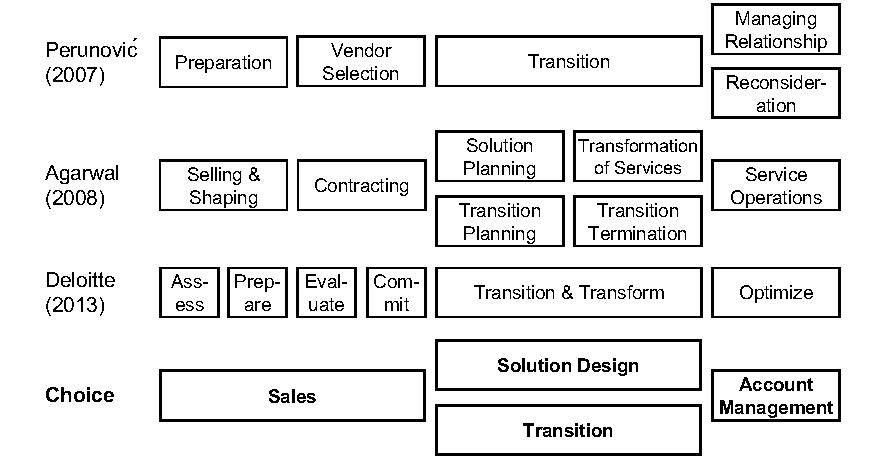
\includegraphics[width=.95\textwidth]{figures/outsourcingprocs.pdf}}
	\end{figure} 
	
	
	\subsection{Sales}
	The contract development step, as in Figure 2, is the formalization of the relationship between outsourced and the outsourcer. \citep{Franceschini_2003}
	
	\subsection{Implementation}
	
	\subsection{Solution Design}
	Deloitte: differentiate between service definition (\ie requirements) and service solution (how provider meets the requirements)
	\subsection{Account Management}
		
\chapter{Demonstration}
%%%%%%%%%%
\label{chap:demo}

\acrshort{DSR} demands a utilization of the artifact in at least one use case. In reference modeling, the model's purpose in practice is its application on a company in the form of an application model. 

Arvato, introduced in chapter \ref{chap:case}, is subject to the instantiation of the domain reference model to a provider model (\cf \Fig \ref{fig:modellevels}). The provider model intentionally embodies individual characteristics, so that changes to the domain reference model are inevitable. These changes specialize, but do not contradict, research in this thesis. 

Documents and interview transcripts are foundation of the following practical exhibition. The interviewees were asked open questions about their business understanding and the reference model was not used to structure the interview in the first place. Consequently, their statements have to be located in the model. 

	\section{Process Framework}
	
	Following a top-down structure, starting point is the most abstract layer of the model.
	 \Tab \ref{tab:interv} gives an overview about covered aspects in interviews. The interviews cover all processes, except \textsc{Inbound Service} and \textsc{Outbound Service}. For these, results from the process modeling workshop are available. The author was part of the workshop and conducted all interviews. 

\begin{table}[caption={Interviews and Relations to Processes}, label={tab:interv}]
	\centering
	
	\begin{tabular}{p{1cm} p{3.4cm}  p{4cm}  p{5cm} }
		\textbf{Order} & \textbf{Topic} & \textbf{Interviewee}          & \textbf{Relation to Processes}                          \\ \hline \hline
		1                            & Model expectations            & Member of the board                  &                                                                         \\\hline
		2                            & Sales                         & Global sales manager                 & \textsc{Sales}, \textsc{Transition}                                                       \\\hline
		3                            & IT                            & Global IT manager                    & \textsc{Transition}                                                              \\\hline
		4                            & Operations                    & Global operations manager            & \textsc{Quality}, \textsc{People Lifecycle}, \textsc{Operations Management} \\\hline
		5                            & Portfolio \& Solution Design  & Global portfolio manager             & \textsc{Product Development}, \textsc{Portfolio Management}, \textsc{Solution Design }             \\\hline
		6                            & Solution Design \& Consulting & Senior consultant                    & \textsc{Product Development}, \textsc{Portfolio Management}, \textsc{Solution Design}              \\\hline
		7                            & Self-Services     & Global portfolio \& solution manager & \textsc{Self-Services}, \textsc{Solution Design}, \textsc{Knowledge Management}                     \\\hline
		8                            & Account Management            & Key account manager                  & \textsc{Transition}, \textsc{Account Management  }                                                    \\\hline
		9                            & Implementation                & Global sales manager                 & \textsc{Transition}                                                             
	\end{tabular}
\end{table}

	Regarding the overall split into management, client and customer processes, interviewees conveyed that Arvato divides into global and local responsibilities.
	Interview partners in a global role reflect on differences between country organizations, while a local view is taken within a country organization. Managerial processes were found on a global level. Client and customer processes were discussed from a global and local perspective. 
	
	Product orientation of Arvato and its competitors was affirmed in the interviews. Compatibility between the understanding of portfolio, products and solutions in this work and at Arvato is given.
	
	 The provider model is shown in \Fig \ref{fig:arvatofram} and detailed in the remainder of this chapter.
	
\begin{figure}[caption={Arvato Framework}, label={fig:arvatofram}]
	{	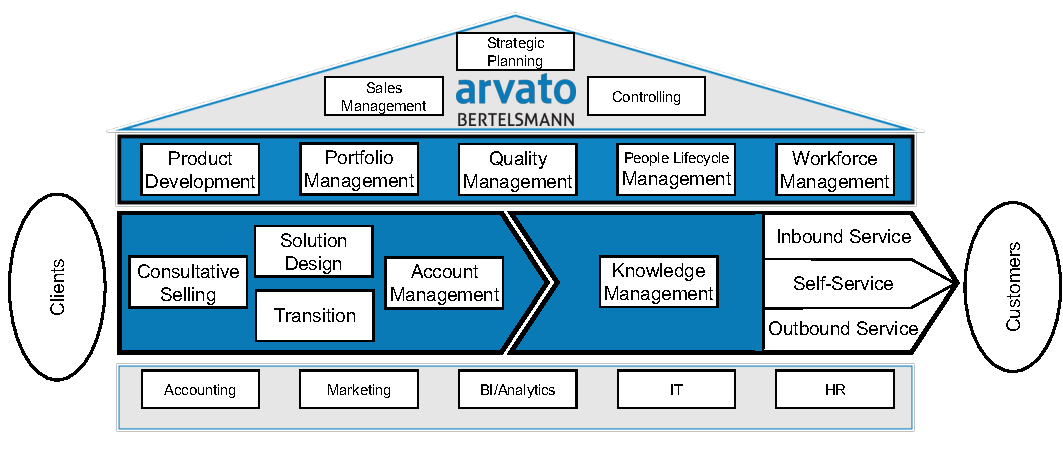
\includegraphics[width=.98\textwidth]{figures/frameworkA.pdf} 
	}
\end{figure}


	%%%%%%%%%%
	%%%%%%%%%%
	
	\section{Customer Processes}
	
	Practical evidence for the four processes in this area is seen in the interview regarding self-services (relating to \textsc{Self-Services} and \textsc{Knowledge Management}) and the process modeling workshop (relating to \textsc{Inbound} and \textsc{Outbound Services}).
	
		\subsubsection{Inbound \& Outbound Services}
	Building on the workshop at one location covering multiple clients in tourism and financial services, a clear picture about operations in a contact center was captured. 
	As voice, video, email, chat, twitter and facebook interactions were covered, all four channel types introduced in this thesis (voice, mail, direct messenger, social) have been explored. As participating managers shared their perception on inter-personal service interactions across client businesses located at their site, an abstraction from client-specific details can be assumed. The outcomes of the workshop were generalized to approximate the detail level within the process reference model. \textsc{Inbound Service} and \textsc{Outbound Service}, as modeled in \ref{pr:inb}, \ref{pr:out}, cover more details than found in the workshop outcomes: As analytical support was very limited and no central customer database was existing, several reference model process steps have to be seen as optional in an application on this client case. However, as one specific client business is seen as a client model instead of a provider model, the supported optionality of process steps in icebricks protects integrity. An omission of these optional steps in the client model can be realized.
	
	\subsubsection{Self-Services \& Knowledge Management}
	The interviewee saw customer needs in center of \textsc{Self-Service}, which is aligned to the reference process. However, it was admitted that difficulties arise in a process representation, because the diversity of self-service utilization implies different procedures. The representation in this work corresponds to the \textit{maintenance} phase of self-service technologies, which follows the \textit{project} phase according to the interviewee. The latter describes the implementation of a self-service and can be seen as part of \textsc{Solution Design} and \textsc{Transition} in the reference model. The maintenance phase especially consists of back-end processes, that are covered in \textsc{Knowledge Management}. Explicitly the creation and maintenance of content \wrt customer needs was mentioned in this regard. The proposed split to case-, transaction-, and customer-related knowledge  in the reference process is hence supported regarding the \textit{case} dimension. In addition, customer- and transaction-related knowledge was deemed important in inter-personal services. 
	
	\textsc{Self-Service} is modeled from a system perspective, therefore it must adequately represent used self-service systems from Arvato. Chat bots and semantic search can be named to give a channel-integrated and stand-alone example. While a chat bot must perform the reference process for every message in a conversion, a single passing through the steps can represent semantic search. The abstract \textit{customer need}  object enables the demonstration of both applications in the reference process.   

	Regarding terminology, the notion \textit{next best action} shall be used instead of \textit{resolution} for Arvato. 
	%%%%%%%%%%
	%%%%%%%%%%
	\section{Client Processes}
	Interviews 2,3,9 and 8 relate to the different stages of the outsourcing lifecycle. \textsc{Solution Design} was part of interview 5,6 and 7 of \Tab \ref{tab:interv}.
	
	While the general structure of the client processes is seen as applicable to Arvato, a customization is applied to emphasize strategic priorities of the organization. \textsc{Sales} is renamed \textsc{Consultative Selling}, as it differentiates Arvato from competitors. 
	
	\subsubsection{Consultative Selling}
	
	This approach puts more emphasis on proactive activities in pre-sales, which is seen in the first two detail processes (\textit{identify prospect} and \textit{approach prospect}). The following steps conform to \textit{Bid Management} at Arvato, where a detailed process description is existing that can be matched with the reference detail processes. For the provider model, this documentation is used to specify process building blocks (\cf Appendix \ref{app:salesbb}). 	The importance of the  \acrshort{RFP} is stressed by Arvato, which conforms to the reference model. \textit{Perform due diligence}, \textit{negotiate contract} and \textit{create commercial deal} are not explicitly listed as parallel processes, but covered in the documentation. %Contract creation is seen as part of \textit{Contract Management} at Arvato. 
	
	\subsubsection{Transition}
	
	Implementation or transition are used to describe the phase between a signed contract and start of final service delivery. As discussed in \ref{pr:tra}, it was affirmed that the process starts during contract finalization, which also supports a separate process on framework level.  A transition plan was not explicitly mentioned, but it can be assumed that information is compiled in one or more documents that structure the transition project. 
	
	The interviewee stated that the most important question in this process is about the location of knowledge and documentation, which is captured in the \textit{transfer business, people, process, technology} detail processes. The proposal to segment into people, process and technology was consented. In addition, the initial recruiting and training of \acrshort{CSR}s was named, which is part of \textsc{People Lifecycle Management} in the reference model. 
	
	While \acrshort{PMO} and \acrshort{TMO} phase were not explicitly mentioned, their concepts were expressed during the interview. It was stated that it is recommended to start the transfer without further changes (corresponding \acrshort{PMO}). After this phase, optimization of status-quo (\ie, \acrshort{TMO}) can be initiated. 
	
	\subsubsection{Account Management}
	 \textsc{Sales} and \textsc{Account Management} can be linked together in country organizations inside Arvato. This view was taken in interview 8 and therefore a scoping of process boundaries was necessary. Starting point of \textsc{Account Management} was seen at the latest with signing of the contract and therefore the process is effective during \textsc{Transition}. Constituents of the reference process were named in the interview, namely service performance monitoring, contract management and especially relationship management. The interviewee emphasized change management, that is not explicitly modeled as a detail process, but captured in \textit{manage disputes}, \textit{propose innovation} and \textit{renegotiate contract}. As a lifecycle analogy was stated, \textit{end contract} is a suitable last detail process. 
          
   	\subsubsection{Solution Design}
	\textsc{Solution Design} as a process in the reference model corresponds to the field of action of a same-named \textit{organizational unit} within the German Arvato organization. This unit also consults in pre-sales activities, that are not part of this process. 
	
	The interviewee stated that starting point during pre-sales is the \textit{identification of potentials for improvement}, from which service requirements are derived. Then, with help of the product portfolio, a client-specific solution is created. The following development is conducted by IT. While the transformation towards a product-oriented organization is aimed, it was admitted that this is work in progress. 
	
	Abstracting from organizational structure, one can state that the described process at Arvato is covered in parts of \textsc{Consultative Selling} and \textsc{Solution Design}. As intended by separate modeling of the \textsc{Solution Design} process, it supports during sales activities. The following justifies the split between consulting and design. 
	
	The reference process starts with \textit{process service challenge}, that assumes challenges are identified in \textsc{Consultative Selling} and used in \textsc{Solution Design} to identify the problem. The specification of these challenges in a proactive or reactive manner is seen as core part of consultative business and consequently must be located as part of \textsc{Consultative Selling}. In turn, designing is focus of \textsc{Solution Design}. 
	
	\section{Management Processes}
	Aim of demonstrating these processes must be their applicability across client businesses, which is embodied through a global pendant at Arvato. Product- and portfolio-related activities fall under responsibility of global \textit{Portfolio \& Solution Design}. It is per definition task of \textit{Operations} to handle service delivery on an executing level. To capture ambitions within Arvato to align operational business across the organization, a global operations initiative was founded to create a framework for harmonization and standardization. Hence, the \textsc{Quality Management}, \textsc{People Lifecycle Management} and \textsc{Operations Management} reference processes must cover their sphere of activity. Available process descriptions were used to enhance detail level. 
	
	Interviews 4 and 5 were subject to processes that strive for alignment across the organization. In addition, documents regarding the available global operations framework are considered for demonstration. A comparison in terms of terminology unveiled that \textsc{Workforce Management} is used instead of \textsc{Operations Management} at Arvato. To foster understanding of the framework, the process is renamed.
	
	%%%%%%%%%%
	\subsubsection{Product Development \& Portfolio Management}
	
	Arvato is in the process of establishing a product orientation. Building a common mindset in differentiating products and solutions is one challenge. Because of this, a separated product development process, isolated from \textsc{Solution Design}, is not defined. However, it was stated that products must be conceptual, derived from market instead of client requirements and the basis for client-specific solution. Essentially, this constitutes the existence of a separate \textsc{Product Development} process as specified in the reference model. 
	
	Awareness for \textsc{Portfolio Management} is existing at Arvato and justified in aspirations to standardize and harmonize \acrshort{CRM} platforms. Furthermore increased transparency was named as one driver, that signifies two views that are taken on the portfolio at Arvato. The \textit{Sales Portfolio} conveys an external view on the products that is communicated towards clients, while the \textit{Delivery Portfolio} links products to internal components and splits these into people, process and platform components. 
	
	A comparison to the reference model demonstrates similarities. With platform components being understood as technology components, the reference model's portfolio structure is a suitable representation of practice at Arvato. 
	In addition to components that relate to one or multiple products, the need of having additional documentation and marketing material was stated, so that a use in \textsc{Solution Design} and \textsc{Consultative Selling} is enabled. 
	
	\subsubsection{Quality Management}
	Quality is deliberately defined widely within this process, so that individual \acrshort{CSR} and overall service delivery performance is covered. The global operations framework lists Staff Performance Management, Quality Management and Client Communication as components, that can be put into relation to the \textsc{Quality Management} reference process. While client communication is part of \textsc{Account Management}, the idea of constant improvement of service delivery is conveyed within \textsc{Quality Management} as well as the reporting function. 
	
	 
	\subsubsection{People Lifecycle Management}
	People, Employee or Agent Lifecycle Management is seen as an integral constituent of HR management in the organization. The mission of People Lifecycle Management at Arvato is the creation of \enquote{a professional environment that attracts the right talent, where performance is rewarded through empowerment, continuous learning and personal development – enabling people to achieve their potential while efficiently and effectively surpassing customer expectations.} However, a detailed process representation was not found. 
	
	To demonstrate the applicability of \textsc{People Lifecycle Management} to the organizational context, lifecycle constituents at Arvato can be compared with reference detail processes. The interviewee mentioned \textit{selecting}, \textit{hiring} and \textit{onboarding} as initial phases, that correspond to the first three steps of the reference process. The following \textit{career path} within Arvato describes the following detail processes and the employee's \textit{attrition} conforms to \textit{let go employee}.
	
	\subsubsection{Workforce Management}
	
	A detailed process description for \textit{Workforce Management} illustrates its similarities to \textsc{Operations Management}. The process at Arvato is composed of \textit{Forecasting} (1), \textit{Capacity Planning} (2), \textit{Scheduling} (3), \textit{Real Time Management} (4) and \textit{Reporting} (5). The first four steps can clearly be mapped to the reference detail processes. The process in the application model is adjusted in form of an additional \textit{perform reporting} detail process and specified process building blocks based on Arvato documents in Appendix \ref{app:wfm}.
	
	
	%\enquote{Putting the right people, with the right skills, in the right place, at the right time, to balance our client expectations, optimize internal efficiencies, while considering our unique employee requirements.}
	
%	plan, execute, control, analyze
%	forecasting, cap plan, scheduling, rtm, analyze
%	external, internal, 

	
	

	
%%%%%%%%%%
\begin{itemize}
	\item Approach from Case advanced to the model itself
	\item ECIS model schemata
	\item type / instance : hybride leistungsbündel
\end{itemize}
\subsubsection{A proposed Architecture for Reference Models in BPO}
	%%%%%%%%%%
	\section{Process Framework}
	%%%%%%%%%%
	\begin{itemize}
		\item meise 2001
	\end{itemize}
	%%%%%%%%%%
	\section{Internal Services}
	%%%%%%%%%%
	%%%%%%%%%%
	\subsection{...}
	%%%%%%%%%%
	%%%%%%%%%%
	\section{Client Services}
	%%%%%%%%%%
	%%%%%%%%%%
	\subsection{...}
	%%%%%%%%%%
	%%%%%%%%%%
	\section{Customer Services}
	%%%%%%%%%%
	Self Service: Servitization paper 1988!
	%%%%%%%%%%
	\subsection{...}
	%%%%%%%%%%
	%%%%%%%%%%
\chapter{Evaluation}
		\chapter{Conclusion}







	%	\chapter{Sample}
This \LaTeX \- template has been developed as an alternative to the well-known Microsoft Word \enquote{Becker-Vorlage}. \path{00_thesis.tex} is the master file.

It is build by  Jan Betzing and Dominik Lekse and draws from the DBIS template by Till Haselmann and Florian Stahl, as well as from the IS template by Stephan Dlugosz.

This document is work-in-progress and provides instructions on how to use the template. It does not give advices on scientific writing.

Please feel free to contribute to this template. Members of the WWU M\"{u}nster can request access to the template by contacting the author at \href{mailto:jan.betzing@ercis.uni-muenster.de}{jan.betzing@ercis.uni-muenster.de}. Afterwards you will be able to clone the template from \path{https://wiwi-gitlab.uni-muenster.de/lsis/isthesis.git}, and create push-requests with their new features.

\paragraph{TODO}
\begin{itemize}
	\item Configuration switch for having \textbackslash chapter\{\} begin on a new page
	\item Replace \texttt{kvoptions} with \texttt{pgfkeys}
\end{itemize}
\section{Elements}
This chapter gives examples on what you can do with this template. It's just a brief overview. Please consult the common sources on how to write sicentific documents and documents with \LaTeX.

\section{Structure}
This template provides three structural levels that appear in the table of contents, \viz, \texttt{\textbackslash chapter}, \texttt{\textbackslash section}, and \texttt{\textbackslash subsection}. Chapters will always start on a new page. Additionally, you can use \texttt{\textbackslash subsubsection} and \texttt{\textbackslash paragraph} as non-hierarchical means to structure your thesis.


\subsection{Lists}
You can use the default \LaTeX \- functions for writing lists, \viz, \texttt{\textbackslash enumerate} for numbered lists and \texttt{\textbackslash itemize} for bullet point lists. Again, the \texttt{\textbackslash subsubsection} and \texttt{\textbackslash paragraph} can be used as structural elements, \eg, when listing definitions of terms.

\subsection{Footnotes}
Footnotes are contiguously numbered throughout the whole document. Use the \texttt{\textbackslash footnote\{text\}} command.  They appear on the page their reference is on \footnote{This is an exemplary footnote.}. Footnotes have to be placed without whitespace behind the word and within the sentence boundaries, \ie, before the period.

\subsection{ToDo-Notes}
You can use ToDo notes using the \texttt{\textbackslash todo\{text\}}  command. Please make sure to remove any ToDo notes before handing in your thesis! \todo[inline]{ToDo: Remove me before publishing}

\section{Formatting Text}
\LaTeX \- provides \texttt{\textbackslash textit\{text\}} for \textit{italics}, \texttt{\textbackslash textbf\{text\}} for \textbf{bold face}, \texttt{\textbackslash texttt\{text\}} for \texttt{typewriter}, \texttt{\textbackslash textsc\{text\}} for \textsc{small caps}, \texttt{\textbackslash underline\{text\}} for \underline{underline}. Additionally, the template provides  \texttt{\textbackslash texthl\{text\}} for \texthl{highlighted text}. Please remove any highlighted text before handing in your thesis!

Please use the \texttt{\textbackslash enquote\{text\}} command for \enquote{direct quotes}.

\subsection{Colors}
This template comes with the colors defined in the  of the \acrshort{ERCIS} and . \Tab \ref{tab:colors} lists the color names. You can apply them to text by using the  \\ \texttt{\textbackslash textcolor\{color name\}\{text\}} command.
	
\begin{table}[caption={Colors defined by the template}, label=tab:colors]
	\centering
		\begin{tabular}{@{}ll@{}}
			\toprule
			{\bf Color Name} & {\bf Result} \\ \midrule
			ercis-black      & \textcolor{ercis-black}{Exemplary Text and 0123456789}  \\
			ercis-grey      & \textcolor{ercis-grey}{Exemplary Text and 0123456789}  \\
			ercis-red      & \textcolor{ercis-red}{Exemplary Text and 0123456789}  \\
			ercis-lightred      & \textcolor{ercis-lightred}{Exemplary Text and 0123456789}  \\
			ercis-blue      & \textcolor{ercis-blue}{Exemplary Text and 0123456789}  \\
			ercis-darkblue      & \textcolor{ercis-darkblue}{Exemplary Text and 0123456789}  \\
			ercis-cyan    & \textcolor{ercis-cyan}{Exemplary Text and 0123456789}  \\
			ercis-orange      & \textcolor{ercis-orange}{Exemplary Text and 0123456789}  \\
			ercis-green      & \textcolor{ercis-green}{Exemplary Text and 0123456789}  \\ \midrule
			wwu-black      & \textcolor{wwu-black}{Exemplary Text and 0123456789}  \\
			wwu-green      & \textcolor{wwu-green}{Exemplary Text and 0123456789}  \\
			wwu-lightgreen      & \textcolor{wwu-lightgreen}{Exemplary Text and 0123456789}  \\
			wwu-blue     & \textcolor{wwu-blue}{Exemplary Text and 0123456789}  \\
			wwu-lightblue      & \textcolor{wwu-lightblue}{Exemplary Text and 0123456789}  \\ \bottomrule
		\end{tabular}
\end{table}


\section{Figures}

The \texttt{figure} environment is wrapped around images. These images should either be included as PDF-file via \texttt{\textbackslash includegraphics}, or created via \textit{TikZ/PGF}. For included images, make sure to use high-resolution images, preferably vector images.

Figures float, \ie, they do not necessarily appear at exact the same position you have defined them. Make sure to set a  \textit{caption} and an optional \textit{label} as figure parameters. 

\begin{figure}[caption={Relationship of students and theses}, label={fig:img01}]
	{	
\includegraphics[width=.6\textwidth]{figures/figure01.pdf}}
\end{figure}

\subsection{Subfigures}
Sometimes it might be handy to contrast figures, \ie, by placing them next to each other. The template uses the \textit{subcaption} package to provide subfigures. The following example contains two figures, where each subfigure has its own \texttt{\textbackslash label} and \texttt{\textbackslash caption}. Additionally, the whole figure has its own \textit{caption} and \textit{label}. That means, you can reference subfigures  \fig \ref{fig:subfig1} and \fig  \ref{fig:subfig}. Only the whole figure will be listed in the table of figures.

Subfigures are not limited to images, but may also include listings or tables. \Fig \ref{fig:subfig} shows a sample database query expressed in  (\fig \ref{fig:subfig1}) and as query plan in relational algebra  (\fig \ref{fig:subfig2}).
 
\begin{figure}[caption={Exemplary use of subfigures}, label={fig:subfig}]
	
	\begin{subfigure}[b]{.45\textwidth}
		
		\begin{lstlisting}[nolol, language=SQL]
		SELECT b, d FROM 
			EXAMPLE.RELATION1 r,
			EXAMPLE.RELATION2 s,
		WHERE 
			r.a = 'c'
		AND 
			s.e = 2
		AND 
			r.c = s.c; 
		\end{lstlisting}
		\caption{select statement}\label{fig:subfig1}
	\end{subfigure}
	\begin{subfigure}[b]{.53\textwidth}
		\centering	
		\begin{tikzpicture}[node distance = 2cm, auto,
		database/.style={
			cylinder,
			cylinder uses custom fill,
			cylinder body fill=gray!30,
			cylinder end fill=gray!20,
			shape border rotate=90,
			aspect=0.25,
			draw
		}]
		\node [] (queue) {$\Pi_{b, d}$};
		\node [below of=queue] (join) {$\Join_{r.c = s.c}$};
		
		\node [below left of=join,xshift=-1cm] (l1) {$\sigma_{r.a = 'c'}$};
		\node [database, below of=l1] (l2) {\texttt{r}};
		
		\node [below right of=join,xshift=1cm] (r1) {$\sigma_{s.e = 2}$};
		\node [database,below of=r1] (r2) {\texttt{s}};
		
		\draw [<-] (queue) -- (join);
		\draw [<-] (join) -- (r1);
		\draw [<-] (r1) -- (r2);
		\draw [<-] (join) -- (l1);
		\draw [<-] (l1) -- (l2);
		\end{tikzpicture}
		\caption{Sample evaluation plan}\label{fig:subfig2}
	\end{subfigure}
\end{figure}
\section{Listings}
You can use listings to typeset source code. This template uses the \textit{listings} package. Wrap code inside the \texttt{lstlisting} environment and set the \textit{language} (e.g., Java, SQL), \textit{caption}, and optional \textit{label} parameters. If the source code highlighting highlights the wrong keywords or misses keywords, use the \textit{deletekeywords} \resp \textit{morekeywords} parameters. Consult the package documentation for further information.

\begin{lstlisting}[float=htp, caption={Euclid's GCD algorithm implemented in Java}, label={lst:euclid}, language=Java, deletekeywords={}, morekeywords={}]
public class Euclid {

	public static int gcd(int p, int q) {
		if (q == 0) return p;
		else return gcd(q, p % q);
	}

}
\end{lstlisting}

\section{Algorithms}
Some users might require specifying algorithms. This template uses the \textit{algorithm}, \textit{algorithmicx}, and \textit{algopseudocode} packages. Consult the respective manuals for further information. Algorithms do not appear in a table at the beginning of the document, \ie, there is no list of algorithms.

\begin{algorithm}[htb]
	\begin{algorithmic}
		\Require nonnegative integer $a$, nonnegative integer $b$
		\Function{Euclid}{$a, b$}
		\If {$b = 0$} \Comment{comment}
		\State{return $a$;}
		\Else 
		\State {return \textsc{Euclid}$(b, a\mod b)$;}
		\EndIf
		\EndFunction
	\end{algorithmic}
	\caption{Euclid's GCD algorithm in pseudocode}
	\label{alg:garbage}
\end{algorithm}

\section{Acronyms and Abbreviations}
This template provides comprehensive support for acronyms and abbreviations. The template uses the \textit{glossaries} package. 
Please do only define abbreviations and symbols that are uncommon. That means, common abbreviations such as \enquote{\eg} or \enquote{\ie} should not be listed. Abbreviations and symbols are sorted automatically by their label. 

\subsection{Common Abbreviations}
Please note that each full stop in a common abbreviation should be followed by a non-breaking space. This template comes with a variety of macros for common abbreviations, that can be used throughout your theses. The macros differ for English and German theses. Please see the tables below.

\begin{table}[caption={Common abbreviation macros for English theses}, label=tab:macros1]
	\centering
	\begin{tabular}{@{}ll@{}}
		\toprule
		{\bf Command} & {\bf Result} \\ \midrule
			\textbackslash apprx      & \apprx \\
			\textbackslash as      & \as \\
			\textbackslash cf      & \cf \\
			\textbackslash eg      & \eg \\
			\textbackslash Eg      & \Eg \\
			\textbackslash esp      & \esp \\
			\textbackslash etal      & \etal \\
			\textbackslash fig      & \fig \\
			\textbackslash Fig     & \Fig \\
			\textbackslash ie      & \ie \\
			\textbackslash Ie      & \Ie \\
			\textbackslash iid      & \iid \\
			\textbackslash p\{4711\}      & \p{4711} \\
			\textbackslash pf\{4711\}      & \pf{4711} \\
			\textbackslash pp\{11$--$47\}      & \pp{11--47} \\
			\textbackslash resp      & \resp \\
			\textbackslash sect     & \sect \\
			\textbackslash tab      & \tab \\
			\textbackslash Tab      & \Tab \\
			\textbackslash viz      & \viz \\
			\textbackslash wrt      & \wrt \\ \bottomrule
	\end{tabular}
\end{table}

\begin{table}[caption={Common abbreviation macros for German theses}, label=tab:macros2]
	\begin{subfigure}[t]{.45\textwidth}
	\centering
	\begin{tabular}{@{}ll@{}}
		\toprule
		{\bf Command} & {\bf Result} \\ \midrule
\textbackslash aaO & \mbox{a.\,a\,O}\xdot \\
\textbackslash Abb & \mbox{Abb.~} \\
\textbackslash bspw & \mbox{bspw}\xdot \\
\textbackslash bzgl & \mbox{bzgl}\xdot \\
\textbackslash bzw & \mbox{bzw}\xdot \\
\textbackslash ca & \mbox{ca}\xdot \\
\textbackslash dgl & \mbox{dgl}\xdot \\
\textbackslash dsgl & \mbox{dsgl}\xdot \\
\textbackslash dh & \mbox{d.\,h}\xdot \\
\textbackslash etc & \mbox{etc}\xdot \\
\textbackslash eV & \mbox{e.\,V}\xdot \\
\textbackslash evtl & \mbox{evtl}\xdot \\
\textbackslash fs & \mbox{f.\,s}\xdot \\
\textbackslash gdw & \mbox{g.\,d.\,w}\xdot \\
\textbackslash ggf & \mbox{ggf}\xdot \\
\textbackslash hc & \mbox{h.\,c}\xdot \\
\textbackslash iAllg & \mbox{i.\,Allg}\xdot \\
\textbackslash iBa & \mbox{i.\,B.\,a}\xdot \\
\textbackslash idR & \mbox{i.\,d.\,R}\xdot \\
\textbackslash ieS & \mbox{i.\,e.\,S}\xdot \\
\textbackslash inkl & \mbox{inkl}\xdot \\
\textbackslash insb & \mbox{insbes}\xdot \\
\textbackslash Prof & \mbox{Prof}\xdot \\
\textbackslash Dr & \mbox{Dr}\xdot \\
\textbackslash PD & \mbox{PD}\xdot \\
\textbackslash Ing & \mbox{Ing}\xdot \\
\textbackslash iV & \mbox{i.\,V}\xdot \\
\textbackslash iW & \mbox{i.\,W}\xdot \\
\textbackslash iwS & \mbox{i.\,w.\,S}\xdot \\
\textbackslash Nr\{123\} & \mbox{Nr.~123} \\
\textbackslash nW & \mbox{n.\,W}\xdot \\
\textbackslash oa & \mbox{o.\,a}\xdot \\
\textbackslash oAe & \mbox{o.\,\"{A}}\xdot \\
			\textbackslash oae & \mbox{o.\,\"{a}}\xdot \\\bottomrule
\end{tabular}
\end{subfigure}
	\begin{subfigure}[position=t]{.45\textwidth}
		\centering
		\begin{tabular}{@{}ll@{}}
			\toprule
			{\bf Command} & {\bf Result} \\ \midrule

			\textbackslash oE & \mbox{o.\,E}\xdot \\
			\textbackslash oEdA & \mbox{o.\,E.\,d.\,A}\xdot \\
			\textbackslash OEdA & \mbox{O.\,E.\,d.\,A}\xdot \\ 
			\textbackslash oV & \mbox{o.\,V}\xdot \\
			\textbackslash OV & \mbox{O.\,V}\xdot \\
			\textbackslash resp & \mbox{resp}\xdot \\
			\textbackslash S\{123\} & \mbox{S.~123} \\
			\textbackslash Sf\{123\} & \mbox{S.~123~f}\xdot \\
			\textbackslash Sff\{123\} & \mbox{S.~123~ff}\xdot \\
			\textbackslash siehe & \mbox{s.\,o}\xdot \\
			\textbackslash sog & \mbox{sog}\xdot \\
			\textbackslash sS\{123\}  & \mbox{s.\,S.~123}\\
			\textbackslash sSf\{123\} &\mbox{s.\,S.~123~f}\xdot \\
			\textbackslash sSff\{123\}& \mbox{s.\,S.~123~ff}\xdot \\
			\textbackslash stu & \mbox{st.\,u}\xdot \\
			\textbackslash su & \mbox{s.\,u}\xdot \\
			\textbackslash Tab & \mbox{Tab.~} \\
			\textbackslash tw & \mbox{t.\,w}\xdot \\
			\textbackslash ua & \mbox{u.\,a}\xdot \\
			\textbackslash etal & \mbox{et\ al}\xdot \\
			\textbackslash uae & \mbox{u.\,\"{a}}\xdot \\
			\textbackslash uAe & \mbox{u.\,\"{A}}\xdot \\
			\textbackslash uiv & \mbox{u.\,i.\,v}\xdot \\
			\textbackslash usw & \mbox{usw}\xdot \\
			\textbackslash uU & \mbox{u.\,U}\xdot \\
			\textbackslash va & \mbox{v.\,a}\xdot \\
			\textbackslash vgl & \mbox{vgl.~} \\
			\textbackslash Vgl & \mbox{Vgl.~} \\
			\textbackslash vs & \mbox{v.\,s}\xdot \\
			\textbackslash zB & \mbox{z.\,B}\xdot \\
			\textbackslash zT & \mbox{z.\,T}\xdot \\
			\textbackslash zz & \mbox{zz}\xdot \\
			\textbackslash zzgl & \mbox{zzgl}\xdot \\
 & \\ \bottomrule
	\end{tabular}
	\end{subfigure}
\end{table}

\subsection{Custom Abbreviations}
Custom abbreviations are defined in the \path{acronyms.tex} file, using the \\
\texttt{\textbackslash newacronym[longplural=\{<long plural>\}, shortplural=\{<short plural>\}]\\ \{<label>\}\{<short>\}\{<long>\}} command. The \textit{longplural} and \textit{shortplural} parameters are optional. The abbreviations are sorted by their labels. The label is furthermore used to reference the abbreviations in your text. You can do so using commands listed in \tab \ref{tab:glossaries}. In most cases, you just use \textbackslash gls\{<label>\}. On the first occurrence, the full version is displayed, \eg, \acrfull{ERCIS}. Afterwards, the short version will be displayed, \eg, \acrshort{ERCIS}.

You pluralize your abbreviation by adding a \texttt{pl} to the \resp command. This will add a small s to the abbreviation, \eg, \acrshortpl{CD}. \Tab \ref{tab:glossaries} shows custom short and long plural versions of the abbreviation \acrshort{kmu}. You might need this \esp for more complex German abbreviations that do not have a \enquote{s} plural form.

\begin{table}[caption={Commands for printing abbreviations}, label=tab:glossaries]
	\centering
	\begin{tabular}{@{}ll@{}}
		\toprule
		{\bf Command} & {\bf Result} \\ \midrule
		\textbackslash gls\{<label>\}     & \textbackslash acrfull on first occurence, \textbackslash acrshort otherwise \\
		\textbackslash glspl\{<label>\}       &  \textbackslash acrfullpl on first occurence, \textbackslash acrshortpl otherwise \\
		\textbackslash acrshort\{<label>\}       & \acrshort{kmu} \\
		\textbackslash acrshortpl\{<label>\}       & \acrshortpl{kmu} \\
		\textbackslash acrlong\{<label>\}       & \acrlong{kmu} \\
		\textbackslash acrlongpl\{<label>\}      & \acrlongpl{kmu} \\
		\textbackslash acrfull\{<label>\}      & \acrfull{kmu} \\
		\textbackslash  acrfullpl\{<label>\}     & \acrfullpl{kmu} \\ \bottomrule
	\end{tabular}
\end{table}

Only referenced abbreviations will be added to the list of abbreviations.

\subsection{Symbols}
If required, you can define symbols in the \path{symbols.tex} file, using the \\ \texttt{\textbackslash addsymboltolist\{<symbol>\}\{<label>\}\{<name>\}} command. The symbols are sorted by their labels. Please note, regardless of using the symbols in the text, all symbols defined in the symbols file will be output to the list of symbols.

\section{Citations and Bibliography}
This template uses {BibTeX} for bibliographies. It comes with the MISQ style that takes care of proper formating and sorting of your references. Of course, you have to maintain a clean \path{.bib} file that caters all necessary attributes. References will appear in the alphabetical order of the surname of the first author. In case of several works by the same author, they are sorted by year.

Citing in the text is done with the \textbackslash citep[<before>][<after>]\{<citekey>\} command. Citations without parenthesis are done with \textbackslash cite\{<citekey>\}. You can reference authors with \textbackslash citeauthor\{<citekey>\}. However, we suggest typesetting authors in \textsc{Small Caps}, \eg, \textsc{\citeauthor{Hammer2015}} is one father of \ac{BPM}.

\paragraph{Exemplary citations}

\begin{itemize}
	\item \gls{BPM} is an integral management paradigm for building and running effective and efficient organizations  \citep{Hammer2015, VomBrocke2014a}.
	\item A holistic approach to \ac{BPM} goes beyond process modeling and workflow management systems \citep[\p{530}]{VomBrocke2014a}.
	\item See \cite{VomBrocke2014a} for a comprehensive review on \ac{BPM} best practices.
	\item \textsc{\citeauthor{Hammer2015}} lists organizational capabilities for \ac{BPM} \citep[\cf][\pf{9}]{Hammer2015}, while \textsc{vom Brocke} \etal give principles of good \ac{BPM} \citep[\cf][\pp{530--546}]{VomBrocke2014a}.
	\item Two authors are automatically divided by an \enquote{and} in English or an \enquote{und} in German, \eg, \citep{Becker2011}.
	\item \enquote{\ac{BPM} can provide a solid set of capabilities essential to master contemporary and future challenges} \citep[\p{534}]{VomBrocke2014a}.
\end{itemize}

\subsection{Misc}
The name and matriculation number of the student will automatically be displayed on the header of every page when the thesis type \textit{seminar} is selected.

\chapter{Compiling the document}
In order to generate a PDF-file from your \TeX-file you have to run the following commands. We assume you have a master file \path{00_thesis.tex} that you want to typeset.


Alternatively, you can use your favorite task runner. This thesis comes with a \textit{Grunt} file to kick-start your \LaTeX writing.

When running, Grunt will monitor your thesis and on file changes, the PDF-file is automatically rebuild using the commands from listing \ref{lst:compiling}.
 
Please make sure to have node.js and the installed. Now you can open a command prompt at the document root and run the commands in listing


\section{Known Issues}
Under some configurations on Windows machines, the \texttt{makeglossaries} command silently fails, which results in empty lists of accronyms and symbols. Same goes for the implicitly called \texttt{makeindex} command. In this case, you have to install \texttt{Perl}\footnote{https://www.perl.org/get.html} on your machine.
		
		
		% Add your content files here
    \end{content}

    % Appendix
     \begin{appendix}
         \section{Customer relationship management}\label{sec:appendix01}

\subsection{CRM notions}
\label{app:crm}
brenneckes crm defs und so 
Appendices provide only two structural levels, \viz, \texttt{\textbackslash section}, and \texttt{\textbackslash subsection}.

Search on scopus, queries are column headings searched in title, abstract and keywords. 

\begin{table}[caption={CRM publication comparison}, label=tab:crmnotioncomparison]
	\centering

	\begin{tabular}{p{1cm}| p{2cm} |p{4.3cm}|p{3cm}   } 
		\textbf{Year} & \textbf{"CRM"} & \textbf{"Customer relationship management"} & \textbf{"Customer Management"} \\ \hline 
		2016          & 211            & 34                                          & 8                              \\
		2015          & 198            & 32                                          & 5                              \\
		2014          & 178            & 35                                          & 4                              \\
		2013          & 193            & 37                                          & 2                              \\
		2012          & 166            & 40                                          & 5                              \\
		2011          & 138            & 44                                          & 7                              \\
		2010          & 131            & 32                                          & 1                              \\
		2009          & 133            & 27                                          & 6                              \\
		2008          & 99             & 22                                          & 2                              \\
		2007          & 118            & 26                                          & 1                              \\
		2006 & 111          & 19                           & 1									 \\
	\end{tabular}
\end{table}

\subsection{Multi- and Omni-channel publications}
\label{app:mcoc}
The search is done on scopus and queries are \enquote{TITLE-ABS-KEY ( ( omnichannel  OR  omni-channel )  AND  ( crm  OR  management  OR  retail )  AND  customer )} and \enquote{TITLE-ABS-KEY ( ( multichannel  OR  multi-channel )  AND  ( crm  OR  management  OR  retail )  AND  customer )}, respectively.

\begin{table}[caption={multi- and omni-channel publication comparison}, label=tab:crmnotioncomparison]
	\centering
	\begin{tabular}{p{1cm}| p{4cm} |p{4cm}    } 
	\textbf{Year} & \textbf{"Multi-channel"} & \textbf{"Omni-channel"} \\ \hline 
	2016          & 32            & 15                                                                       \\
	2015          & 33            & 10                                                                   \\
	2014          & 30            & 7                                                                   \\
	2013          & 17            & 1                                                           \\
	2012          & 24            & 1                                                              \\
	2011          & 24            &                                                       \\
	2010          & 25            &                                                                \\
	2009          & 34            &                                                       \\
	2008          & 29             &                                             \\
	2007          & 23            &                                                       \\
	2006 & 29         &                           					 \\
\end{tabular}
\end{table}

\subsection{Multi- and Omnichannel separation}
\label{app:mcoc2}
	Separating multi-channel from omni-channel is difficult, as the latter formed as an amplification of the former. \cite{vorhoef2015retail} try a distinction shown in Table \ref{tab:mcoccomparison}, which is here masked from the retail domain. 
\begin{table}[caption={Multi- and omni-channel comparison}, label={tab:mcoccomparison}]
	\centering
	\begin{tabular}{p{3cm}| p{5cm} |p{5cm}} 
		& \textbf{Multi-channel management}                                   & \textbf{Omni-channel management}                                                              \\ \hline
		\textit{Channel focus}                         & \textit{Interactive channels only}                                    & \textit{Interactive and mass-communication channels}                                                   \\ \hline
		\textit{Channes scope}                                 & \textit{Store, online website and direct marketing}                          & \textit{In addition mobile channels (\ie, smart phone, tablets, apps), social media}                   \\ \hline
		{Separation of channels}                           & Separate channels with no overlap                                  & Integrated channels providing seamless customer experiences                                   \\ \hline
		{Brand versus channel customer relationship focus} & Customer - channel focus                                            & Customer - channel - brand  focus                                                              \\ \hline
		{Channel management}                               & Per channel                                                         & Cross-channel                                                                                 \\ \hline
		{Objectives}                                       & Channel objectives (\ie sales per channel, experience per channel)& Cross channel objectives (\ie, overall customer experience, total sales over channels) \\
		
	\end{tabular}
	\quelle{Adapted from \citep[\p{176}]{vorhoef2015retail}}
\end{table}
Aspects in channel focus and scope can be criticized in this juxtaposition. It is questionable that channels are excluded from multi-channel management, because in essence the distinction is seen in the relationship \textit{between} channels and not the channels themselves. The excluded channels from multi-channel management (\viz, mass communication) go back to the channel definition of \cite{Neslin2006}, which emphasizes interaction between customer and company. From this, \citeauthor{vorhoef2015retail} infer that solely two-way communication channels can be part of multi-channel management. The understanding in this work is different and makes no difference in possible channel focus and scope among omni- and multi-channel management. As \citeauthor{vorhoef2015retail} describe multi- and omni-channel as \enquote{phases}, they put mobile channels and social media as additions from multi- to omni-channel. This view might be reasoned in the publication time, because multi-channel publications in the early 2000s could not predict the impact of smart phones and tablets on marketing, as the more recent omni-channel publications. Appendix \ref{app:mcoc} holds an overview about publications over time regarding omni- and multi-channel management and proves the greater impact of multi-channel management over omni-channel management in the literature. 


\subsection{Outsourcing Provider Processes}
\label{app:provproc}

		\begin{figure}[caption={Outsourcing provider processes}, label={fig:scheweproc}]
	{	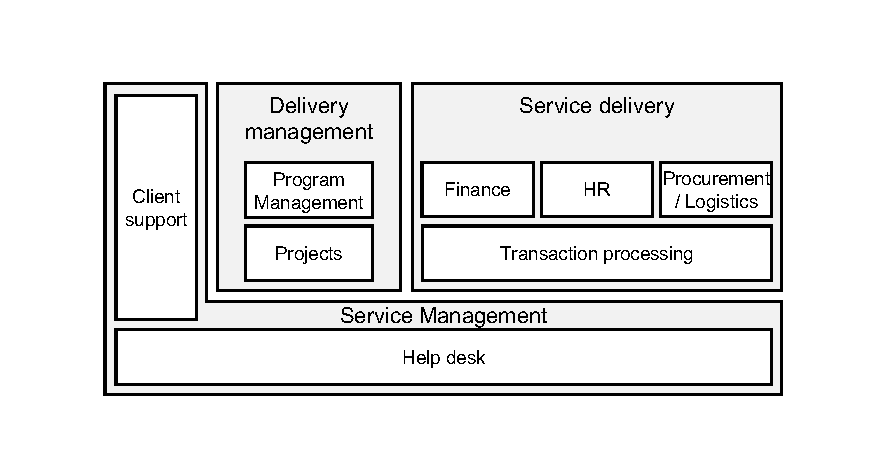
\includegraphics[width=.8\textwidth]{figures/scheweproc.pdf}\\
		\quelle{\citep[\p{98}]{schewe2007}} } 
\end{figure}
\subsection{Selected Reference Models}

\label{app:refmods}
	\begin{figure}[caption={SCOR Model}, label={fig:scor}]
	{	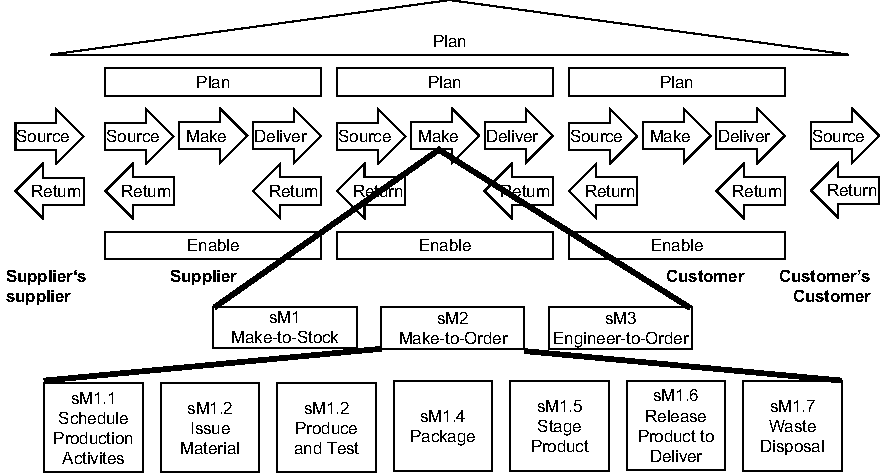
\includegraphics[width=.8\textwidth]{figures/scor.pdf}\\
	\parbox{.8\textwidth}{\quelle{\citep{APICS2015}}}} 
\end{figure}

	\begin{figure}[caption={Retail-H}, label={fig:retailh}]
	{	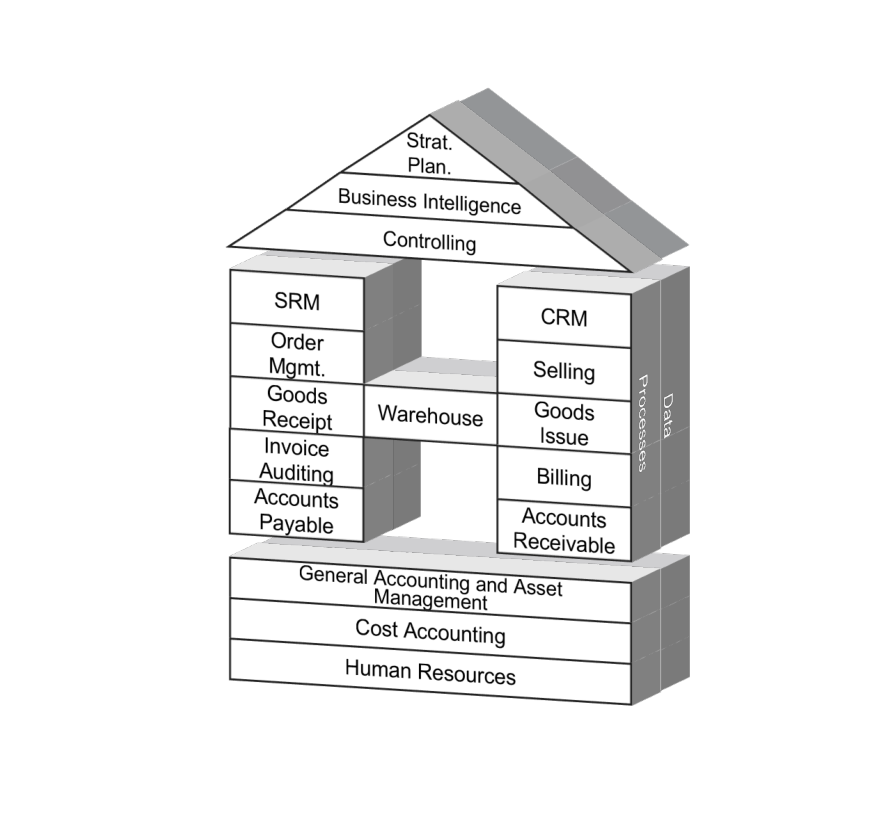
\includegraphics[width=.6\textwidth]{figures/retailh.pdf}
	\\ \parbox{0.6\textwidth}{\quelle{\citep{becker2004handelsinformationssysteme}}}}

	
\end{figure}

\subsection{icebricks Example}
\label{app:iceb}
\begin{figure}[caption={icebricks process structure example: Retail-H \acrshort{CRM} process}, label={fig:soldes}]
	\begin{subfigure}[c]{.32\textwidth}
		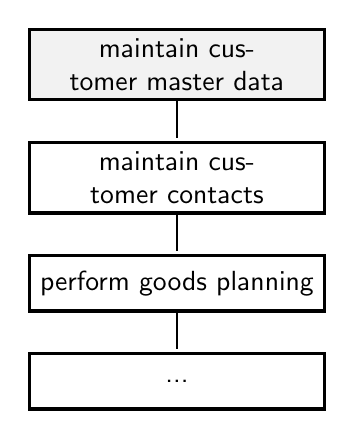
\begin{tikzpicture}
		[node distance=.5cm, start chain=going below,font=\sffamily]
		\node[punktchain, rounded corners=0pt, fill= gray!10, join=by {-}] (eins)      {maintain customer master data};
		\node[punktchain, rounded corners=0pt, join=by {-}] (zwei)      {maintain customer contacts};
		\node[punktchain, rounded corners=0pt, join=by {-}] (drei)      {perform goods planning};
		\node[punktchain, rounded corners=0pt, join=by {-}] (drei)      {...};
		\end{tikzpicture}
		\caption{selection of CRM process components (detail processes)}\label{fig:retailh:main}
	\end{subfigure}
\begin{subfigure}[c]{.05\textwidth}
	\begin{tikzpicture}
	\end{tikzpicture}
\end{subfigure}
	\begin{subfigure}[c]{.45\textwidth}
		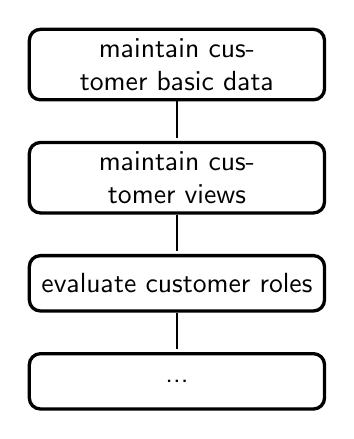
\begin{tikzpicture}
		[node distance=.5cm, start chain=going below,font=\sffamily]
		\node[punktchain, join=by {-}] (eins)      {maintain customer basic data};
		\node[punktchain,join=by {-}] (zwei)      {maintain customer views};
		\node[punktchain,  join=by {-}] (drei)      {evaluate customer roles};
		\node[punktchain,  join=by {-}] (drei)      {...};
		\end{tikzpicture}
		\caption{selection of maintain customer master data shows process building blocks}\label{fig:retailh:detail}
	\end{subfigure}
	
\end{figure}

\subsection{Knowledge Management frameworks}
\label{app:knowmang}

\begin{table}[caption={Knowledge Management Framework options}, label=tab:knowmangoptions]
	\centering
	
	\begin{tabular}{p{1cm}| p{2cm} |p{2cm}|p{3cm} | p{5cm  } }
		\textbf{Year} & \textbf{Author} & \textbf{Type} & \textbf{Decision} & \textbf{Activities} \\ \hline 
		2000          & Andersen Consulting            &      Technical Report                                      & \text{\sffamily X} URL not found         & Acquire, Create, Synthesize, Share, Use to Achieve                     \\
		1999          & Knowledge Associates            & Technical Report                                       &  \text{\sffamily X} URL not found & Acquire, Develop, Retain, Share                             \\
			1997          & Van Heijst \etal            & Paper                                          &  \checkmark & Development, Consolidation, Distribution, Combination                              \\
		1996          & Marquardt            & Book                                          &  \text{\sffamily X} Book not available & Acquisition, Creation, Transfer \& Utilization, Storage                             \\
	


	\end{tabular}
	\quelle{adapted from \citep[\pf{8}]{Rubenstein_Montano_2001}}
\end{table}
\subsection{Financial engineering in the outsourcing deal}
\label{app:fineng}
	\begin{figure}[caption={Financial engineering in the outsourcing deal}, label={fig:scheweproc}]
	{	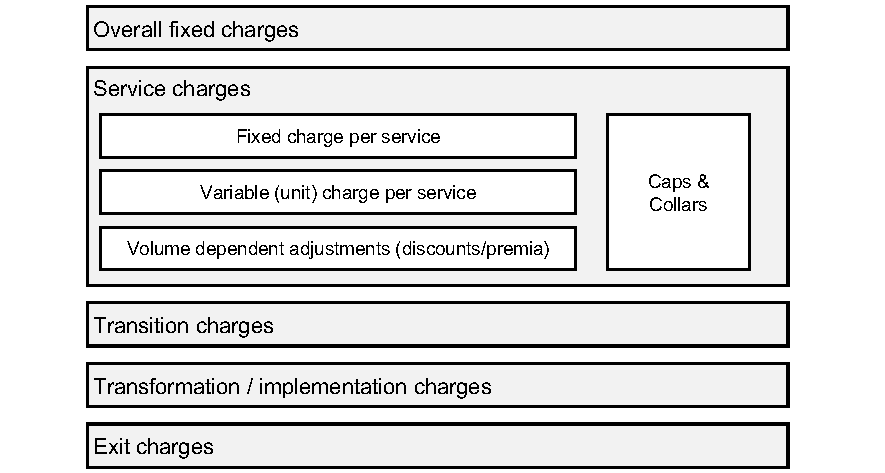
\includegraphics[width=.8\textwidth]{figures/financialengineering.pdf}
		
 }
 \parbox{.6\textwidth}{\quelle{\citep[\p{32}]{deloittehandbook}}}

\end{figure}


\subsection{Frameworks for the Product Development process}
\label{app:pdframeworks}
% Please add the following required packages to your document preamble:
% \usepackage{multirow}
\begin{table}[caption={Product Development process derivation}, label=tab:nsdframeworkds]
	\centering
\begin{tabular}{p{4cm}|p{5cm} |p{4.7cm}}
	\textbf{\cite{cowell1988new}} & \textbf{\cite{Edgett_1996}} adapted from \cite{cooper1988new}  & \textbf{Process in thesis}   \\ \hline \hline
	idea generation                 &                                         \\ \hline
	idea screening                  & idea screening   & evaluate idea                      \\ \hline
	& \textbullet \: preliminary market assessment     &assess market requirements    \\
	& \textbullet \: preliminary technical assessment  &assess technical requirements       \\
	& \textbullet \: detailed market study / market research \\ \hline
	concept development and testing &                       & conceptualize product                  \\ \hline
	business analysis               & business/financial analysis           & perform business analysis  \\ \hline
	\multirow{4}{*}{development}    & \textbullet \: product development      &	\multirow{4}{*}{develop product}               \\ 
	& \textbullet \: process procedures                      \\
	& \textbullet \: system design \& testing                \\
	& \textbullet \: personell training                      \\\hline
	testing                         & test market / trial sell       & test product         \\ \hline
	                      & pre-commercialization \:\:\:\:\:\:\:\:\:\:\:\:\:\:\:\:\:\:\: business analysis \\ \hline
	commercialization               & full-scale launch                   & deliver product    \\ \hline
	& post-launch review \& analysis         
\end{tabular}\\
\quelle{adapted from \citep{Edgett_1996, cowell1988new}}
\end{table}

\subsection{Some Appendix Subsection}

\lipsum[10]
     \end{appendix}

    % References
    \references{library}

    % Declaration of authorship
    % \authorshipstatement[pagenumbering=false]    \authorshipstatement[pagenumbering=true]
    % \authorshipstatement[pagenumbering=only]
    
    % Bonus: Wordcount
    % cd %FOLDER WHERE THE .tex FILES ARE IN %
    % clear
    % texcount -total -q -col -sum *.tex
    
\end{document}